%%%%%%%%%%%%%%%%%%%%%%%%%%%%%%%%%%%%%%%%%
% The Legrand Orange Book
% LaTeX Template
% Version 3.0 (January 26, 2022)
%
% This template originates from:
% https://www.LaTeXTemplates.com
%
% Authors:
% Vel (vel@latextemplates.com)
% Mathias Legrand (legrand.mathias@gmail.com)
%
% License:
% CC BY-NC-SA 4.0 (https://creativecommons.org/licenses/by-nc-sa/4.0/)
%
% Compiling this template:
% This template uses biber for its bibliography and makeindex for its index.
% When you first open the template, compile it from the command line with the 
% commands below to make sure your LaTeX distribution is configured correctly:
%
% 1) pdflatex main
% 2) makeindex main.idx -s indexstyle.ist
% 3) biber main
% 4) pdflatex main x 2
%
% After this, when you wish to update the bibliography/index use the appropriate
% command above and make sure to compile with pdflatex several times 
% afterwards to propagate your changes to the document.
%
%%%%%%%%%%%%%%%%%%%%%%%%%%%%%%%%%%%%%%%%%

%----------------------------------------------------------------------------------------
%	PACKAGES AND OTHER DOCUMENT CONFIGURATIONS
%----------------------------------------------------------------------------------------

\documentclass[
	11pt, % Default font size, select one of 10pt, 11pt or 12pt
	fleqn, % Left align equations
	a4paper, % Paper size, use either 'a4paper' for A4 size or 'letterpaper' for US letter size
	%oneside, % Uncomment for oneside mode, this doesn't start new chapters and parts on odd pages (adding an empty page if required), this mode is more suitable if the book is to be read on a screen instead of printed
]{LegrandOrangeBook}

% Book information for PDF metadata, remove/comment this block if not required 
\hypersetup{
	pdftitle={Title}, % Title field
	pdfauthor={Author}, % Author field
	pdfsubject={Subject}, % Subject field
	pdfkeywords={Keyword1, Keyword2, ...}, % Keywords
	pdfcreator={LaTeX}, % Content creator field
}


\newsavebox{\fminipagebox}
\NewDocumentEnvironment{fminipage}{m O{\fboxsep}}
 {\par\kern#2\noindent\begin{lrbox}{\fminipagebox}
  \begin{minipage}{#1}\ignorespaces}
 {\end{minipage}\end{lrbox}%
  \makebox[#1]{%
    \kern\dimexpr-\fboxsep-\fboxrule\relax
    \fbox{\usebox{\fminipagebox}}%
    \kern\dimexpr-\fboxsep-\fboxrule\relax
  }\par\kern#2
 }

\addbibresource{sample.bib} % Bibliography file

\definecolor{ocre}{RGB}{52, 134, 235} % Define the color used for highlighting throughout the book
\providecommand{\tightlist}{%
  \setlength{\itemsep}{0pt}\setlength{\parskip}{0pt}}
\chapterimage{orange1.jpg} % Chapter heading image
\chapterspaceabove{6.5cm} % Default whitespace from the top of the page to the chapter title on chapter pages
\chapterspacebelow{6.75cm} % Default amount of vertical whitespace from the top margin to the start of the text on chapter pages

%----------------------------------------------------------------------------------------

\begin{document}

%----------------------------------------------------------------------------------------
%	TITLE PAGE
%----------------------------------------------------------------------------------------

\titlepage % Output the title page
	{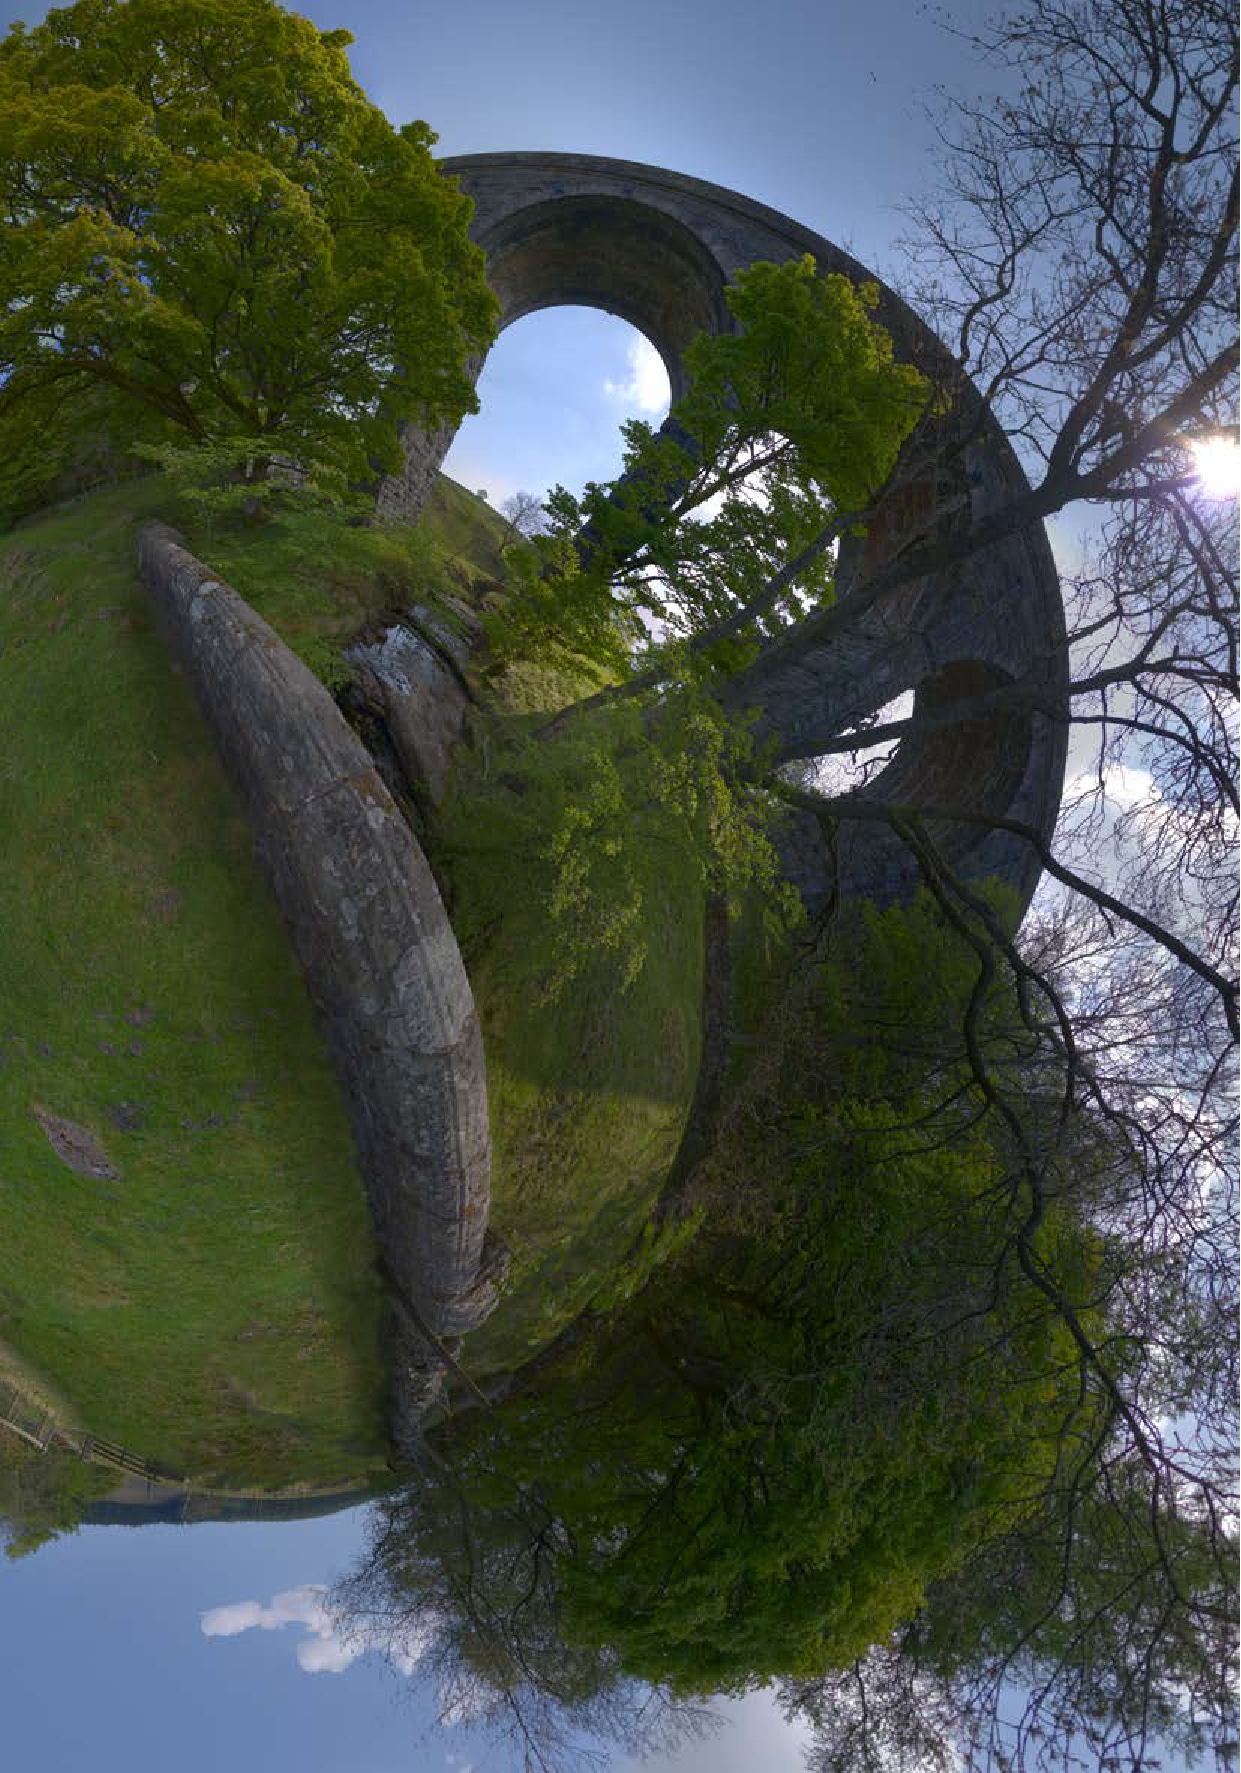
\includegraphics[width=\paperwidth]{background.pdf}} % Code to output the background image, which should be the same dimensions as the paper to fill the page entirely; leave empty for no background image
	{ % Title(s) and author(s)
		\centering\sffamily % Font styling
		{\Huge\bfseries Money in Metaverses\par} % Book title
		\vspace{16pt} % Vertical whitespace
		{\LARGE Bitcoin in global social immersive mixed reality systems\par} % Subtitle
		\vspace{24pt} % Vertical whitespace
		{\huge\bfseries John O'Hare \& Allen Fairchild\par} % Author name
	}

%----------------------------------------------------------------------------------------
%	COPYRIGHT PAGE
%----------------------------------------------------------------------------------------

\thispagestyle{empty} % Suppress headers and footers on this page

~\vfill % Push the text down to the bottom of the page

\noindent \href{https://creativecommons.org/publicdomain/zero/1.0/}{No Copyright}\\ 2022 John O'Hare \& Allen Fairchild\\ % Copyright notice

\noindent \textsc{Published by j.ohare@salford.ac.uk for the Cyber Foundry Programme at The University of Salford}\\ % Publisher

\noindent \textsc{\href{https://raw.githubusercontent.com/GMCyberFoundry/Metaverse/main/Paper/metaverseBTC.pdf}{Raw GitHub hyperlink}}\\ % URL

\noindent The person who associated a work with this deed has dedicated the work to the public domain by waiving all of his or her rights to the work worldwide under copyright law, including all related and neighboring rights, to the extent allowed by law.\\
You can copy, modify, distribute and perform the work, even for commercial purposes, all without asking permission. See Other Information below.\\
This license is acceptable for Free Cultural Works.
Other Information\\
In no way are the patent or trademark rights of any person affected by CC0, nor are the rights that other persons may have in the work or in how the work is used, such as publicity or privacy rights.\\
Unless expressly stated otherwise, the person who associated a work with this deed makes no warranties about the work, and disclaims liability for all uses of the work, to the fullest extent permitted by applicable law.\\
When using or citing the work, you should not imply endorsement by the author or the affirmer.



\noindent \textit{First printing, March 2022} % Printing/edition date

%----------------------------------------------------------------------------------------
%	TABLE OF CONTENTS
%----------------------------------------------------------------------------------------

\pagestyle{empty} % Disable headers and footers for the following pages

\tableofcontents % Output the table of contents

\listoffigures % Output the list of figures, comment or remove this command if not required

\listoftables % Output the list of tables, comment or remove this command if not required

\pagestyle{fancy} % Enable default headers and footers again

\cleardoublepage % Start the following content on a new page

%----------------------------------------------------------------------------------------
%	PART
%----------------------------------------------------------------------------------------

\part{State of the art and proposal}

%----------------------------------------------------------------------------------------
%	SECTIONING EXAMPLES CHAPTER
%----------------------------------------------------------------------------------------

\chapterimage{orange2.jpg} % Chapter heading image
\chapterspaceabove{6.75cm} % Whitespace from the top of the page to the chapter title on chapter pages
\chapterspacebelow{7.25cm} % Amount of vertical whitespace from the top margin to the start of the text on chapter pages

%------------------------------------------------

\section{Conflict of interest statements}
The authors may own small numbers of the various tokens referenced in the text for experimentation and/or investment purposes. At this time that is only sufficient Ethereum to operate a Web3 wallet, and Bitcoin locked on the Lightning network. No NFTs are owned at this time. There are no financial stakes in the development of any of these ecosystems.
\chapter{Introduction}
\section{Abstract}
We present a state of the art and positioning book, about Web3, Bitcoin, and `Metaverse'; describing the intersections and synergies. A high level overview of Web3 technologies leads to a description of blockchain, and the Bitcoin network is specifically selected for detailed examination. Suitable components of the extended Bitcoin ecosystem are described in more depth. Other mechanisms for native digital value transfer are described, with a focus on `money'. Metaverse technology is over-viewed, primarily from the perspective of Bitcoin and extended reality.\\
Bitcoin is selected as the best contender for value transfer in metaverses because of it's free and open source nature, and network effect. Challenges and risks of this approach are identified. A cloud / virtual machine technology stack can be downloaded and deployed from GitHub to experiment with the technologies, with a focus on cybersecurity best practice. This deployable lab is designed to inform development of secure value transaction, for small and medium sized companies. Next steps are touched upon in the conclusion.\\
\textbf{This is an incomplete document and may frankly contain a bunch of errors. Usual v0.1 caveats apply. It's 100\% opensource (unlicense) so if something seems wrong pertaining to your project, or you have a suggestion for an improvement, then submit a PR to GitHub. There's a bunch of place holder text using the Lorem Ipsum insert from LaTeX. If you see that, skip to the end of the section. Targeting April 2022 for a final draft. 20 working days left.}
\section{Introduction}
This document presents a high level view of technologies and potential within the emergent Web3 and metaverse narrative, focusing around the transmission of value within and across such global networks, with a further focus on the Bitcoin monetary network. It was written to organise the thoughts of the authors, who were unfamiliar with Bitcoin technologies until recently.\\
As adoption of these technologies increases it will be necessary for people, and AI actors, to pass economic value between themselves. These `goods and services' interactions, within the virtual social spaces, should be underpinned by a trust system, which scales globally, and presents low friction. Current secure international payment rails are poorly suited to such interactions; indeed it is likely with legacy systems, that parties would be forced to leave the metaverse application, and instead navigate their banking applications to exchange value with overseas entities in a secure fashion. This might conceivably take several days.\\ 
Fortunatly, the whole landscape of money and \href{https://www.omfif.org/futureofpayments2021/}{value transfer is changing}. Huge global financial players are entering the space. The world's largest pension fund manager Blackrock is adding these asset to their management engine which managed tens of trillions of dollars. Of their recent investments KPMG global said:\\
\textit{``We've invested in a strong cryptoassets practice and we will continue to enhance and build on our capabilities across Decentralized Finance (DeFi), Non-Fungible Tokens (NFTs) and the Metaverse, to name a few''}. \\
Meanwhile Google have \href{https://blog.youtube/inside-youtube/innovations-for-2022-at-youtube/}{recently blogged}:\\
\textit{``Web3 also opens up new opportunities for creators. We believe new technologies like blockchain and NFTs can allow creators to build deeper relationships with their fans. Together, they’ll be able to collaborate on new projects and make money in ways not previously possible. For example, giving a verifiable way for fans to own unique videos, photos, art, and even experiences from their favorite creators could be a compelling prospect for creators and their audiences. There’s a lot to consider in making sure we approach these new technologies responsibly, but we think there’s incredible potential as well. Finally, we couldn’t have a piece about innovation without touching on the metaverse! We're thinking big about how to make viewing more immersive. ''}\\
This is has immediate implications for SMEs. It is timely then to explore the potential of recent technologies, which can address metaverse interactions in \textit{business to business} (B2B), \textit{business to customer} (B2C), and the newer C2C (social commerce; \textit{creator to consumer, customer to customer, consumer to consumer\cite{jones2008trust})}. Figure \ref{fig:landscapevenn} demonstrates how some of these domains intersect.\\ 
This book seeks to overview and explain the available open source technologies. It supports an open source \href{https://github.com/GMCyberFoundry/Metaverse}{github repository} which enables SMEs to access these emergent platforms and ecosystems. It aims to build toward a minimum viable product for trust minimised transfer of value within a social immersive space.\\
Referencing is in two styles; academic works are numeric, while opinion pieces, grey stats, and pertinent news articles are hyperlinked in blue from the text. As the book develops the veracity of the citations should improve. It is likely that this document is incomplete as you are reading it as it's designed to be an open ended and open source resource. It is an experiment in a living document and repository.

\begin{figure*}[ht]\centering % Using \begin{figure*} makes the figure take up the entire width of the page
	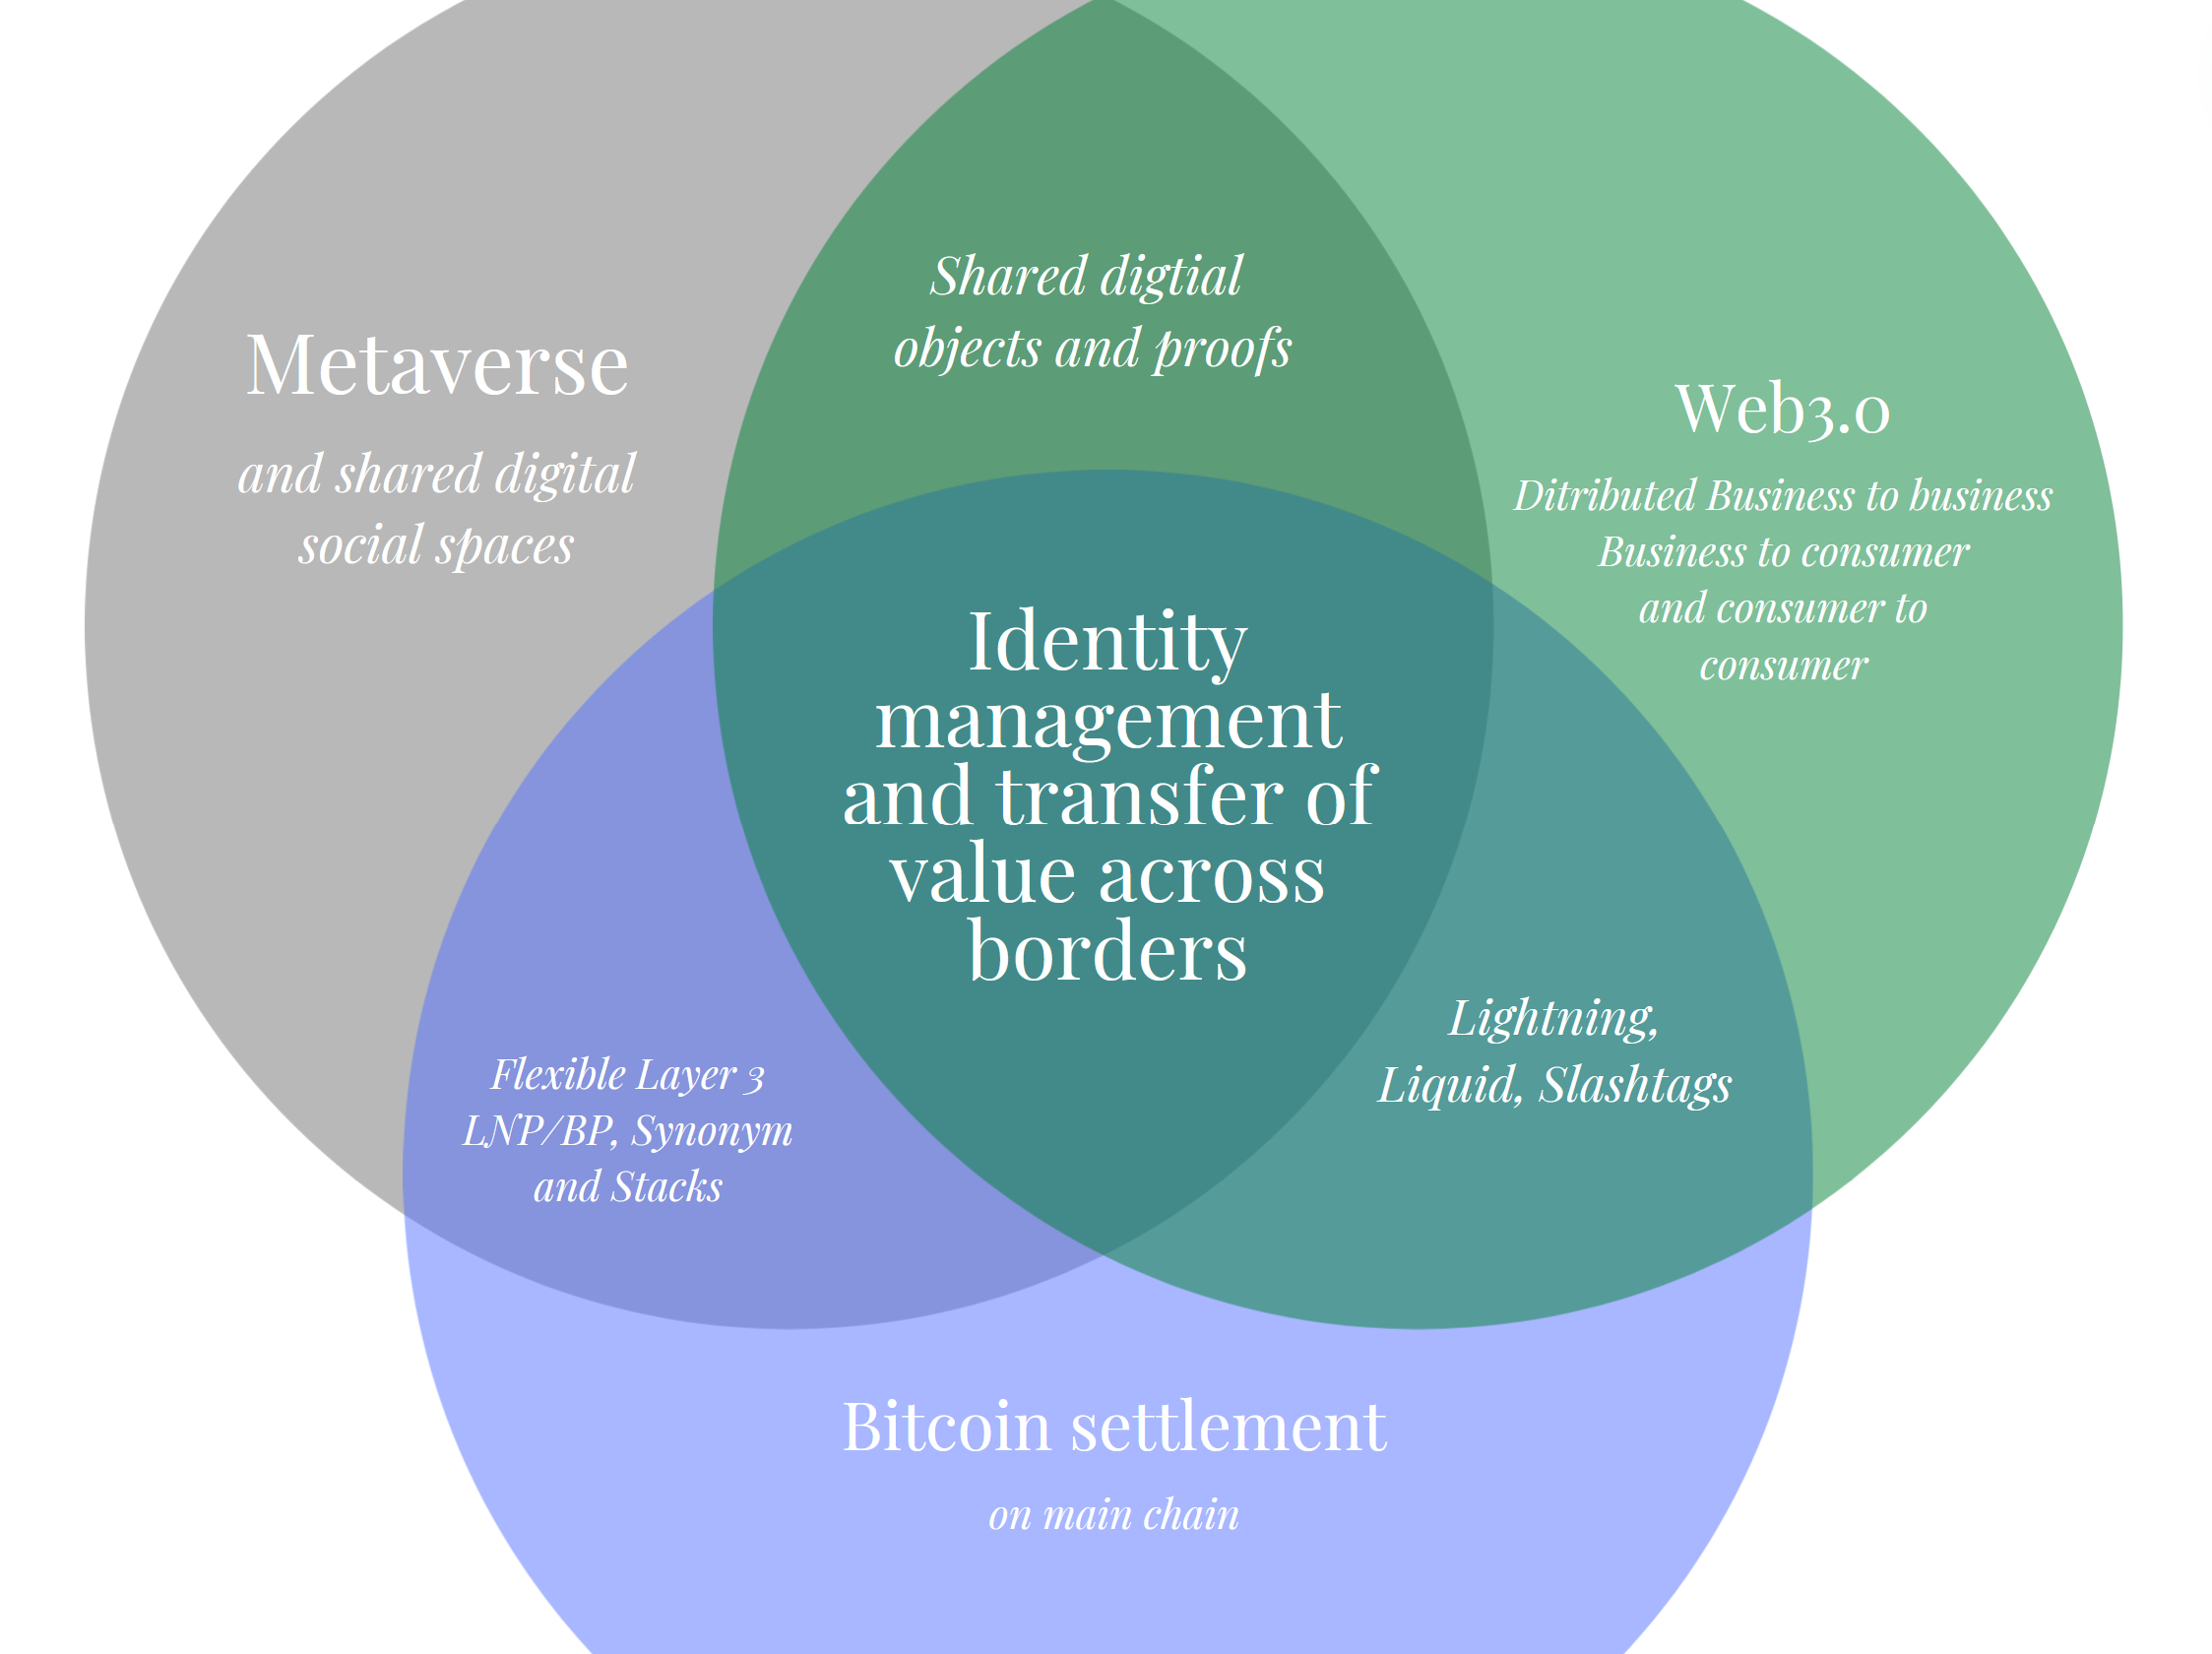
\includegraphics[width=\linewidth]{landscapevenn}
	\caption{Web 3, Metaverse, and Bitcoin are inter-sectional technologies.}
	\label{fig:landscapevenn}
\end{figure*}
\chapter{Web3 / decentralised web}
Web3 is a rapidly evolving set of technologies and specifications which are drifting further from their origin. Decentralised web is perhaps a more useful name, but focus in this section will be on the evolution of the popularised term Web3. 
\section{Semantic web}
The ``semantic web'' definition of Web3.0 has been somewhat overhauled by other innovations in decentralised internet technologies, now evolving toward the slightly different Web3 moniker. Tim Berners Lee (of WWW fame) first mentioned the semantic web in 1999 \cite{semanticWeb}.\par
``I have a dream for the Web [in which computers] become capable of analyzing all the data on the Web – the content, links, and transactions between people and computers. A "Semantic Web", which makes this possible, has yet to emerge, but when it does, the day-to-day mechanisms of trade, bureaucracy and our daily lives will be handled by machines talking to machines. The "intelligent agents" people have touted for ages will finally materialize.''\par
Attention developed around three core themes, ubiquitous availability and searchability of data, intelligent search assistants, and highly available end points such as phones, and `internet of things' devices. This is certainly manifesting in home devices, but few people think of this as a Web3 revolution. The framework can be seen in Figure \ref{fig:semanticWebStack}.\par
\begin{figure}
  \centering
    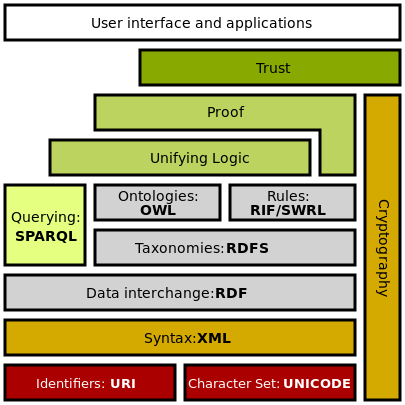
\includegraphics[width=\linewidth]{semanticWebStack}
  \caption{\href{https://en.wikipedia.org/wiki/Semantic_Web_Stack}{Semantic Web Stack} [CC0 image]}
  \label{fig:semanticWebStack}
\end{figure}
Since ratification of the standards by the \href{https://www.w3.org/standards/semanticweb/}{World Wide Web (W3C) consortium} it seems that their imperative toward decentralisation has become lost. Instead, it can be seen that Facebook, Amazon, Google, and Apple have a harmful oligopoly on users data \cite{costigan2018world}. This is as odds with Berners-Lee's vision. \par
It is worth taking a look at his software implementation called \href{https://solidproject.org}{Solid}, which is far more mindful of the sovereignty of user data.\par
``Solid is an exciting new project led by Prof. Tim Berners-Lee, inventor of the World Wide Web, taking place at MIT. The project aims to radically change the way Web applications work today, resulting in true data ownership as well as improved privacy. Solid (derived from "social linked data") is a proposed set of conventions and tools for building decentralized social applications based on Linked Data principles. Solid is modular and extensible and it relies as much as possible on existing W3C standards and protocols.'' \par
Excitement around this kind of differentiated trust model, hinted at in ubiquitous availability of data (and implemented explicitly in Solid), has led to exploration of different paths by cryptographers, and this will be described later. For instance, one of the main developers of Solid, Melvin Carvelho, is now a lead developer at Nostr, another very interesting option which will be described later. This technology space is prolific, but still comparatively young and small.\par
\section{Spatial web}
``The Spatial Web'', a blurring of the boundaries between digital and geospatial physical objects, seems to have developed from the strands in the original W3C scope around devices in the real world. It has been concentrating around AR and VR but is being marketed and amplified with the same references to availability of data (See Figure \ref{fig:deloitteSpatial} from a Deloitte accounting report). This too is finding little traction in practice, though obviously the component technologies continue to enjoy rapid development. Nonetheless, this interpretation of Web3 becomes valuable when examining Metaverse later.\par
\begin{figure}
  \centering
    \includegraphics[width=\linewidth]{deloitteweb3}
  \caption{\href{https://www2.deloitte.com/us/en/insights/topics/digital-transformation/web-3-0-technologies-in-business.html}{Deloitte Spatial Web Overview} Reused with permission.}
  \label{fig:deloitteSpatial}
\end{figure}
\section{Web3}
More recently Web3 is \href{https://trends.google.com/trends/explore?date=all&q=web3}{being touted} as a way to connect content creators directly to content consumers, without centralised companies acting as gatekeepers of the data. It implies that all users have a cryptographic key management system, to which they attach metadata, that they make requirements of peers with whom they communicate, and that they maintain trust `scores' with peers.\par
It seems likely that this new model is less driven by a market need, and more by the high availability of tools which allow this to happen (the ecosystems described later). Add to this a social response to the \href{https://finance.yahoo.com/news/meta-facebook-worst-company-of-the-year-yahoo-finance-165345819.html}{collapse in trust of companies such as Facebook} (Figure \ref{fig:trustbarometer}), a wish by consumers to pass more of the economic incentive to content creators, without the `rent seeking' layer afforded by businesses, and a healthy dose of mania driven market speculation. 

\begin{figure}
  \centering
    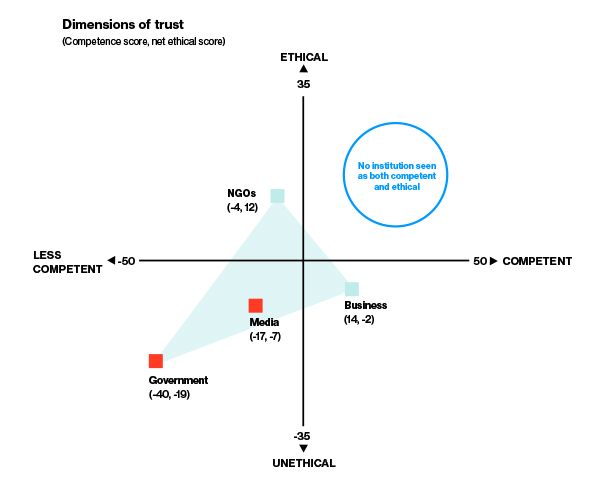
\includegraphics[width=\linewidth]{c-a-e}
  \caption{\href{https://www.edelman.com/trust/2020-trust-barometer}{Edelman 2020 trust barometer} [rights requested]}
  \label{fig:trustbarometer}
\end{figure}
\subsection{Emerging consensus}
It's possible to frame Web3 as a hugely complex and inefficient digital rights management system (DRM). DRM is something that users of the internet are increasingly familiar and comfortable with. It's somewhat debatable whether decentralising this is worthwhile. The thesis of the developers of the technology seems to be that without it, control of `value' will accrete over time, to one or more hegemonic controlling entities. It's a strong argument, but there is a \href{https://moxie.org/2022/01/07/web3-first-impressions.html}{substantial counter argument} emerging that users just don't want this stuff. The nervousness of legislators in the USA to the attempt by Facebook/Meta to enter this peer-to-peer value transmission space is telling in terms of the perception of who is driving Web3.\par
At the end of 2021 and the beginning of 2022 there is much furore on the internet over what Web3 might be, and who it `serves'. 
Enthusiasts feel that products such as \href{https://blog.spruceid.com/sign-in-with-ethereum-is-a-game-changer-part-1/}{Sign-In with Ethereum} (EIP-4361) will give users choice over their data sovereignty, and a meme to this effect is seen in Figure \ref{fig:web1web2web3}. In practice though users are expecting to use badly written, buggy, economically vulnerable `crypto' wallets to log into websites. It doesn't seem to make much sense yet on the face of it. There are in fact examples of the technology completely failing at censorship resistance. Popular `Web3' browser extension Metamask and NFT platform Opensea have both \href{https://www.forbes.com/sites/stevenehrlich/2022/03/03/iranian-venezuela-users-abruptly-dropped-from-major-crypto-platforms-as-russian-sanctions-grow/?sh=22bcabc470b0}{recently banned countries} in response to global sanction pressure. This failure to meaningfully decentralise will be explored further in the distributed identity section. \par
\begin{figure}
  \centering
   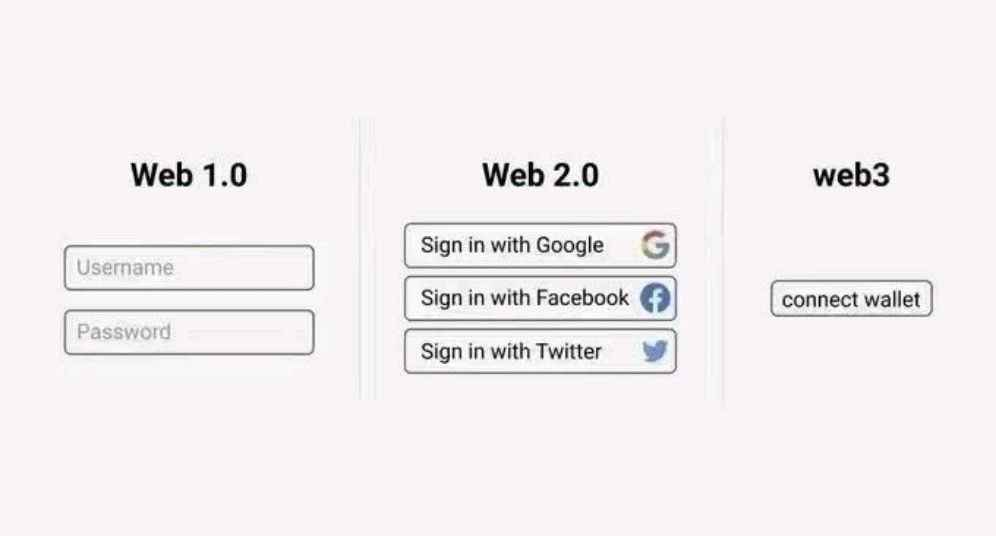
\includegraphics[width=\linewidth]{web1web2web3}
 \caption{A meme showing differing approached to logging in on a website.}
 \label{fig:web1web2web3}
\end{figure}
The current hype cycle is ignoring the legacy definitions described above and instead focusing almost exclusively on Ethereum based peer-to-peer projects (more on these later). It can be seen that the description is somewhat in the eye of the beholder.\par
This new hyped push for Web3 is being driven by enormous venture capital investment. A16Z are a \href{https://a16z.com/2022/01/07/9b-to-build-the-future/}{major player} in this new landscape and have released their \href{https://a16z.com/2022/01/07/how-to-build-a-better-internet-10-principles-for-world-leaders-shaping-the-future-of-web3/}{ten principles} for emergent Web3. 
\begin{itemize}
\item Establish a clear vision to foster decentralized digital infrastructure
\item Embrace multi-stakeholder approaches to governance and regulation
\item Create targeted, risk-calibrated oversight regimes for different web3 activities
\item Foster innovation with composability, open source code, and the power of open communities
\item Broaden access to the economic benefits of the innovation economy
\item Unlock the potential of DAOs
\item Deploy web3 to further sustainability goals
\item Embrace the role of well-regulated stablecoins in financial inclusion and innovation
\item Collaborate with other nations to harmonize standards and regulatory frameworks
\item Provide clear, fair tax rules for the reporting of digital assets, and leverage technical solutions for tax compliance
\end{itemize}
This list seems targeted toward the coming regulatory landscape, and could be considered at odds with the original tenants of an organically emergent, decentralised internet. Indeed principles such as `furthering sustainability goals' seem downright incongruous. The community they claim to wish to support here are openly critical of these major institutional players and their motives. This book and lab steer well clear of these companies and their applications.\par
Dante Disparte, chief strategy officer of Circle, said in testimony to a US senate hearing; that Web 1 was `read', Web 2 was `read write', and that Web 3 will `read write own'. The important takeaway here is not so much this oft quoted elevator pitch for Web3, but the fact that legislative bodies now consider this technology a force which they need to be aware of and \href{https://a16z.com/2021/12/17/prediction-for-the-new-year-a-web3-midterm/}{potentially contend with}.\par
Jeremy Allaire of `Circle' venture capital talks about the recent legislative order in the USA as follows:
\textit{``this is a watershed moment for crypto, digital assets, and Web 3, akin to the 1996/1997 whole of government wakeup to the commercial internet. The U.S. seems to be taking on the reality that digital assets represent one of the most significant technologies and infrastructures for the 21st century; it's rewarding to see this from the WH after so many of us have been making the case for 9+ years.''}\par
\href{https://www.finder.com/uk/cryptocurrency-statistics}{It's estimated} that about 6\% of people in the UK own some cryptocurrency, with skews to both younger demographics, and smaller holdings. The legislative landscape in the UK is comparatively strict with strong ``know your customer / anti money laundering'' (KYC/AML) data collection \href{https://www.gov.uk/guidance/money-laundering-regulations-your-responsibilities}{mandated in law}. Users of UK exchanges must provide a great deal of personal financial information, and undertake to prove that the wallets they are withdrawing to are their own. Europe meanwhile has recently voted through even more restrictive regulation, applying the ``\href{https://www.europarl.europa.eu/legislative-train/theme-an-economy-that-works-for-people/file-revision-of-the-regulation-on-transfers-of-funds}{transfer of funds regulation}'' to all transactions coming out of exchanges, enforcing a database of all addresses, and reporting transactions above 1000 Euros to authorities. This onerous overhead will likely make it impossible for smaller businesses in the sector to operate within the EU.\par
%Many of the mentioned components here will be described later in the book. The suggestion is that this is happening regardless of a decent use case or definition.\par
It's a complex evolving narrative, and clearly contradictions are common. Into this confusion this book advances a narrow take, and toolset, which might extract some value from the technologies, while maintaining a low barrier to entry.\par 

\section{Example applications}
\subsection{Podcasting2.0}
\href{https://medium.com/@everywheretrip/an-introduction-to-podcasting-2-0-3c4f61ea17f4}{Podcasting 2.0} leverages RSS (the original dissemination system for podcasts) and the Bitcoin Lightning network, to enable so-called `value for value' broadcasting. Subscribers use one of a variety of apps to stream micro-transactions of Bitcoin directly to the content creators as they listen to the podcast. No intermediate business takes a cut. Some variation on this model exists, such as John Carvalho's crowd funded podcast ``The Biz'' which progressively unlocks more minutes for everyone based on \href{https://thebiz.pro/about#crowdwall}{crowd funded donations}.
\subsection{Crowd funding}
At time of writing a \href{https://www.constitutiondao.com/}{crowd funding initiative} based around a digital decentralised construct called a DAO (explained later in detail) \href{https://www.coindesk.com/business/2021/12/06/daos-and-the-next-crowdfunding-gold-rush/}{managed to raise \$46 million dollars to bid for a copy of the US constitution} at Southerbys auction house. The attempt narrowly failed, but the press \href{https://www.coindesk.com/business/2021/12/09/what-kickstarter-going-decentralized-means-for-web-3/}{heralded this new era of ``Web3'' economic might}. This model might be the only use for DAOs and is likely just a way to avoid regulatory scrutiny. There is more detail on DAOs later.
\subsection{Distributed exchanges}
There are dozens of decentralised exchanges deployed on various blockchains. These platforms allow users to trade back and forth between various tokens (including `normal money' stablecoins) and charge a fee for doing so. They operate within the logic of the smart contracts, within the distributed blockchains. This makes them extremely hard to ban, and as a result they operate in a legal grey area. At the extreme end of this is ``distributed apps'' (dApps) and ``Decentralised Finance'' (DeFi) which allows users access to complex financial instruments without legal or privacy constraints. DeFi will be touched on briefly later.\par
This is a huge area, and of only limited interest to the topics expanded in this book. It's perhaps worth noting \href{https://bitcoin-dex.net/about/index.html}{BitcoinDEX}, which runs in JavaScript in a web browser. It is effectively uncensorable, \href{https://bitcoin-dex.net/tokens.js}{auditable by the user}, and has no counter party risk since it operates entirely in the Bitcoin network. It is clearly an early prototype but manages this complex feature without the more expressive logic of more `modern' public blockchains.
\subsection{NFT marketplaces}
NFT markets are far more centralised services which match `owners' of digital assets with potential buyers. The concept is a staple of the more recent interpretation of Web3, even though in practice these seem to be centralised concerns. \href{https://opensea.io/}{Opensea} claims to be the largest decentralised NFT marketplace, but they have the ability to \href{https://thedefiant.io/sad-frogs-delisted-opensea/}{remove listings} in response to legal challenges. This seems to fly in the face of Web3 principles. NFTs are currently a \href{https://tante.cc/2021/12/17/the-third-web/}{deeply flawed} technology but seem likely to persist and will be covered later.
\subsection{Slashtags / Hypercore}
Slashtags is a web of trust model decentralised peer-to-peer model which assigns metadata and trust scores to `any' data and connection, with a security model rooted in the Bitcoin cryptographic `keys' but crucially not the bitcoin network. This makes it interoperable with bitcoin but not reliant upon it. In principle this allows users to build complex networks of inherited trust bi-directionally with their networks over time. Every connection to a peer can be a new schema, with individual metadata managed by the user. It is new and has low adoption at this time. The user controls the source of the data and can allow them to be used by centralised services. This flips the authentication and data management paradigm of Web2 around, putting the user in charge of their data. This is a familiar concept to the DID/SSI communities (described later) but with significant investment. As Slashtags use keys as endpoints they act as a web of naming and routing, bypassing the existing web infrastructure of DNS. It is likely very complex to use in practice and will be revisited later. It is being paired with the \href{https://hypercore-protocol.org/}{Hypercore protocol} for peer-to-peer data sharing, more specifically the `hole punching' capability of the hypercore system which ensures connections through firewalls\cite{ford2005peer}. The first application by the affiliated Hyperdivision team is an open source peer-to-peer live video streaming app called \href{https://dazaar.com/}{Dazaar}. Once again, it's not clear yet who wants or needs this bit-torrent style service. 
\subsection{Distributed DNS applications} 
There are many perceived problems with having centralised authorities for overseeing the database which translates between human readable internet names and the underlying machine-readable address notation. The databases which manage this globally are already somewhat distributed, and this distributed trust model is managed through a cryptographic chain of trust called DNSSEC which is capped by a somewhat \href{https://www.iana.org/dnssec/ceremonies}{bizarre key ceremony}. The authority around naming is centralised in ICANN. There has been talk for many years about `properly' distributing this database using decentralised/blockchain technologies\cite{karaarslan2018blockchain}. The nature of this problem means that it either moves from control by ICANN, or it does not, and so far it has not, but there are many attempted and somewhat mature attempts at this difficult problem. Of these \href{https://www.namecoin.org/}{Namecoin} is the most prominent, and is a fork of Bitcoin. The ubiquity of Bitcoin in such systems is perhaps becoming apparent.
\subsection{Impervious browser}
It might be that the future of Web3 comes in the guise of integrated suites such as the proposed \href{https://newsletter.impervious.ai/impervious-browser-functionality-overview/}{Impervious web browser}. They say that ``without centralized intermediaries'' it features:
\begin{itemize}
\item    Zoom, without Zoom.
\item    Google Docs, without Google.
\item    Medium, without Medium.
\item    WhatsApp, without WhatsApp.
\item    Payments, without banks.
\item    Identity, without the state.
\end{itemize}
This is obviously leading marketing hype, but what they're talking about here is an integration of the components mentioned in this book. If they can get critical mass around this browser then perhaps the Web3 market can be kickstarted.
\section{The common thread}
One feature which persists throughout all of these interpretations of Web3 is the need for decentralised trust. According to \href{https://www.coindesk.com/podcasts/the-breakdown-with-nlw/yesterdays-hearing-was-cryptos-most-positive-interaction-with-the-us-government-ever/}{Nathaniel Whittemore}, a journalist for Coindesk, ``The Web3 moniker positions this industry in opposition to big tech''. In practice it seems that this is just another avenue for existing players to experiment with new \href{https://www.cigionline.org/articles/amid-the-hype-over-web3-informed-skepticism-is-critical/}{models of control and monetisation}, as in \href{https://stripe.com/gb/use-cases/crypto}{this announcement} from Stripe, the worlds biggest payment processor. Overall, the space is hype, and \href{https://web3isgoinggreat.com/}{rife with scams}. The degree to which it currently accomplished decentralised trust is very debatable.\par
With that said the component part necessary to deliver on this promise \textbf{do} exists. If there is to be no central controlling party(s) as in the Web 2 model then nothing can happen without a cryptographically secure underpinning, allowing digital data to be passed around without a prior arrangement.\par%which favours no party beyond the terms of their collectively agreed rights and privileges. 
The rest of this section will describe how much has been done by computer scientists over the past decades to support that. From this base layer we also get the potential for secure and trust minimised identity management. This nascent field of distributed identity management is explained later. From distributed trust models we can see `trustless' transmission of economic value. The ability to send value from one person to another person or service without a third party. \par
This whole area is `crypto', which is increasingly seeping into the human consciousness, and saw an astonishing \$30B of \href{https://docsend.com/view/nrvsuae85a4dx3jz}{capital investment in 2021} alone. At time of writing the industry is a \href{https://www.coingecko.com/en}{over 2 trillion} dollar market. \par
Of their 2022 \href{https://research.ark-invest.com/thank-you-big-ideas-2022?submissionGuid=0937b1ae-9e11-4b46-ae03-6cd8d2f8301b}{`Big Ideas' report}, ARK investment LLC (who manage a \$50B tech investment) \href{https://www.ark-bigideas.com/2022/en/pages/download}{said the following} (Figure \ref{fig:ARKWeb3}), which connects some of the dots already mentioned, and leads us into the next section which is Blockchain and Bitcoin:\par
\textit{``While many (with heavily vested interests) want to define all things blockchain as web3 we believe that web3 is best understood as just 1 of 3 revolutions that the innovation of bitcoin has catalyzed.
\begin{itemize}
\item The Money Revolution
\item The Financial Revolution
\item The Internet Revolution''
\end{itemize}}
\begin{figure}
  \centering
    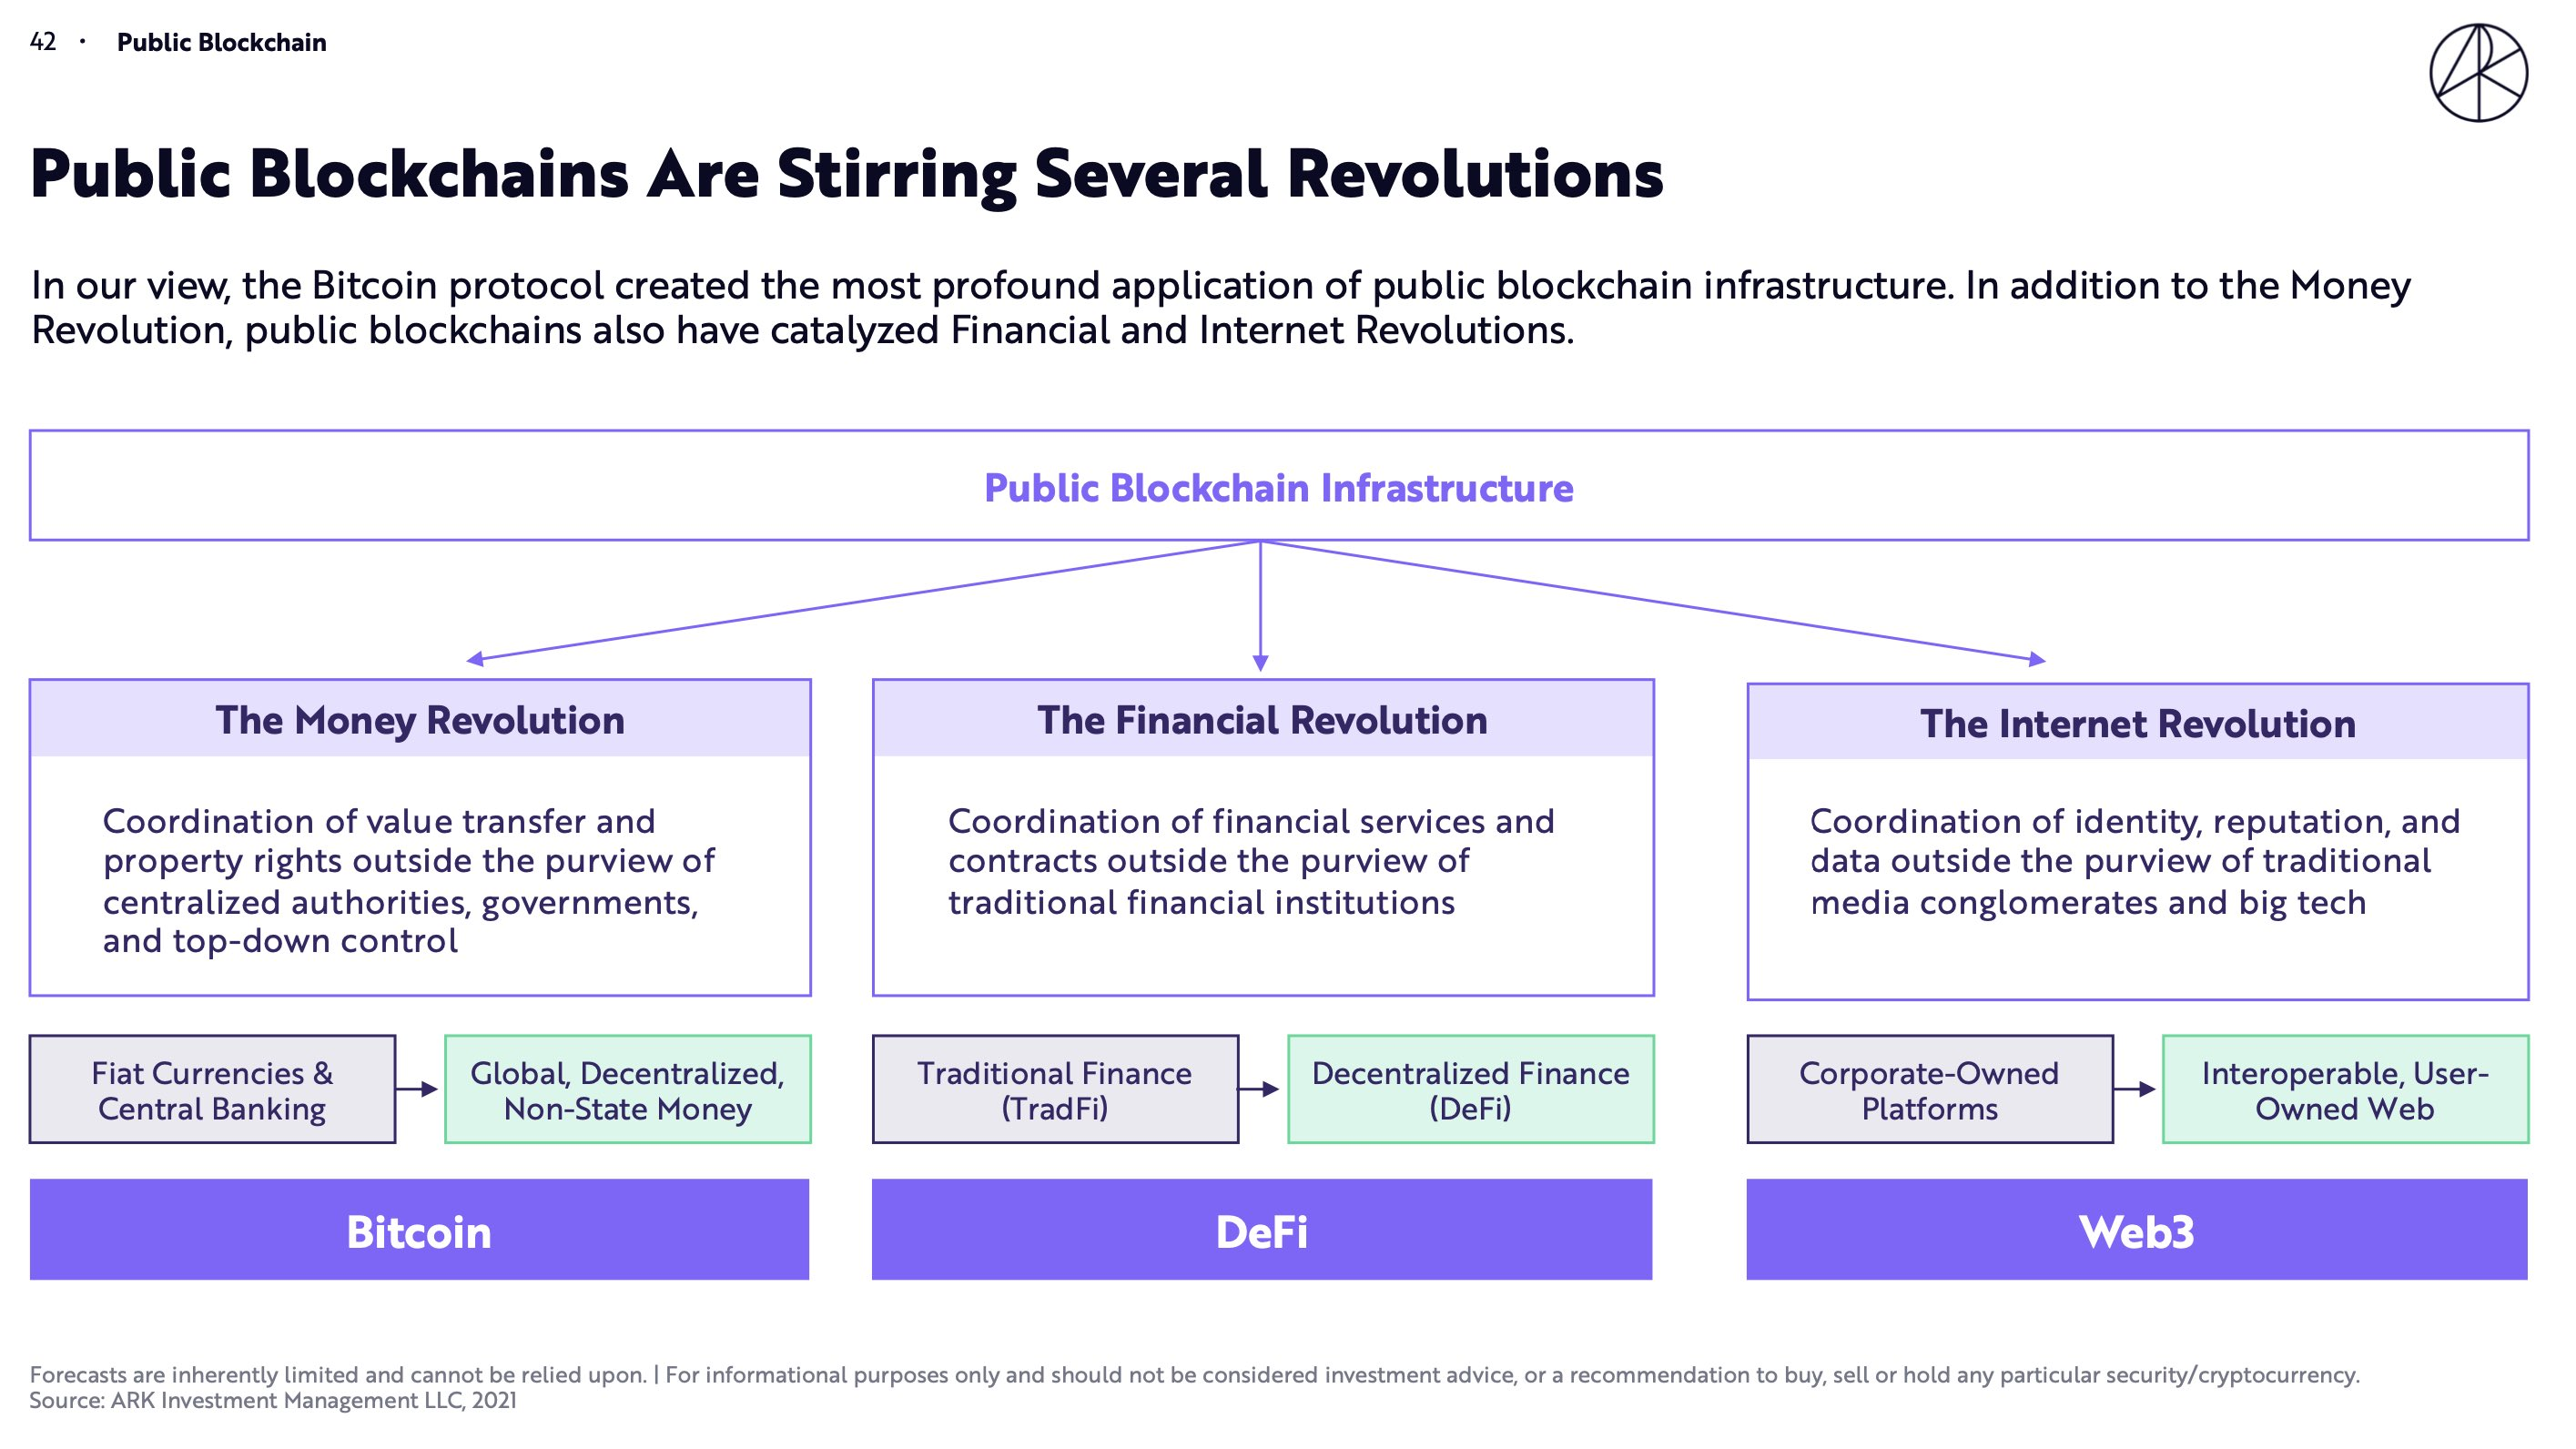
\includegraphics[width=\linewidth]{Web3ARK}
  \caption{\href{https://twitter.com/wintonARK/status/1486143239753060353}{ARK slide on Web3.} Rights requested}
  \label{fig:ARKWeb3}
\end{figure}
All the new crypto technologies circling the Web3 narrative are bound tightly together, but there is currently very little meaningful value to be seen.\par
The rest of this book will focus on the trust and value transfer elements of this shift in internet technologies, and attempt to build a case for it's use in decentralised, open source, metaverse applications.
%\section{Risks}

\chapter{DLT, Blockchain, and Bitcoin}
Distributed ledger technology (DLT) is a data structure distributed across multiple managing stakeholders. A subset of DLT is blockchain, which is a less efficient, immutable data structure with a slightly different trust model. Rauchs et al. of the Cambridge Centre for Alternative Finance provide a detailed taxonomy and conceptual framework \cite{rauchs2018distributed}. It can be seen in their paper that the definitions are somewhat unclear in literature.\\
DLT, and especially blockchain, are rapidly gaining ground in the public imagination, within financial technology companies (FinTech), and in the broader corporate world. \\
The technology and the global legislative response are somewhat immature, and misapplications of both technologies are commonplace. \\
Distributed trust models emerged from cryptography research in the 1970s when Merkle, Diffie, and Hellman at Stanford figured out how to \href{https://medium.com/swlh/understanding-ec-diffie-hellman-9c07be338d4a}{send messages online} without a trusted third party \cite{diffie1976new,merkle1978secure}.\\
Soon after the 1980s saw the emergence of the cypherpunk activist movement, as a reaction to the emerging surveillance state \cite{burnham1983rise, chaum1985security}. These early computer scientists in the USA saw the emerging intersectionality between information, computation, economics, and personal freedom \cite{lavoie1990prefatory}. Online discussion in the early nineties foresaw the emergence of trans-national digital markets, what would become the WWW \cite{salinCosts, cypherPunkMailList}. The issues of privacy %(https://nakamotoinstitute.org/static/docs/cypherpunk-manifesto.txt) 
 and the exchange of digital value (digital / ecash)%(https://www.wired.com/1994/12/emoney/  https://www.cs.ru.nl/~jhh/pub/secsem/chaum1985bigbrother.pdf) 
 were of foremost importance within these discussions %(https://www.wired.com/1994/12/emoney/), 
 and while privacy was within reach thanks to ``public/private key pairs'' %(https://www.openpgp.org/about/history/), 
 ecash proved to be a more difficult problem. \\
Adam Back's 1997 `hashcash' \cite{back2002hashcash} paved the way for later work by introducing the concept of `proof of work'. This was built upon by Dai \cite{dai1998b}, Szabo \cite{szabo1997formalizing}, Finney \cite{callas1998openpgp}, and Nakamoto amongst others. In all it took 16 years of collaboration on the mailing lists to attack the problem of trust minimised, distributed, digital cash. The culmination of these attempts were Bitcoin \cite{Nakamoto2008}. This is illustrated by Dan Held in Figure \ref{fig:prehistory}. \\
This is now a wider ecosystem of technologies. 

\begin{figure}
  \centering
    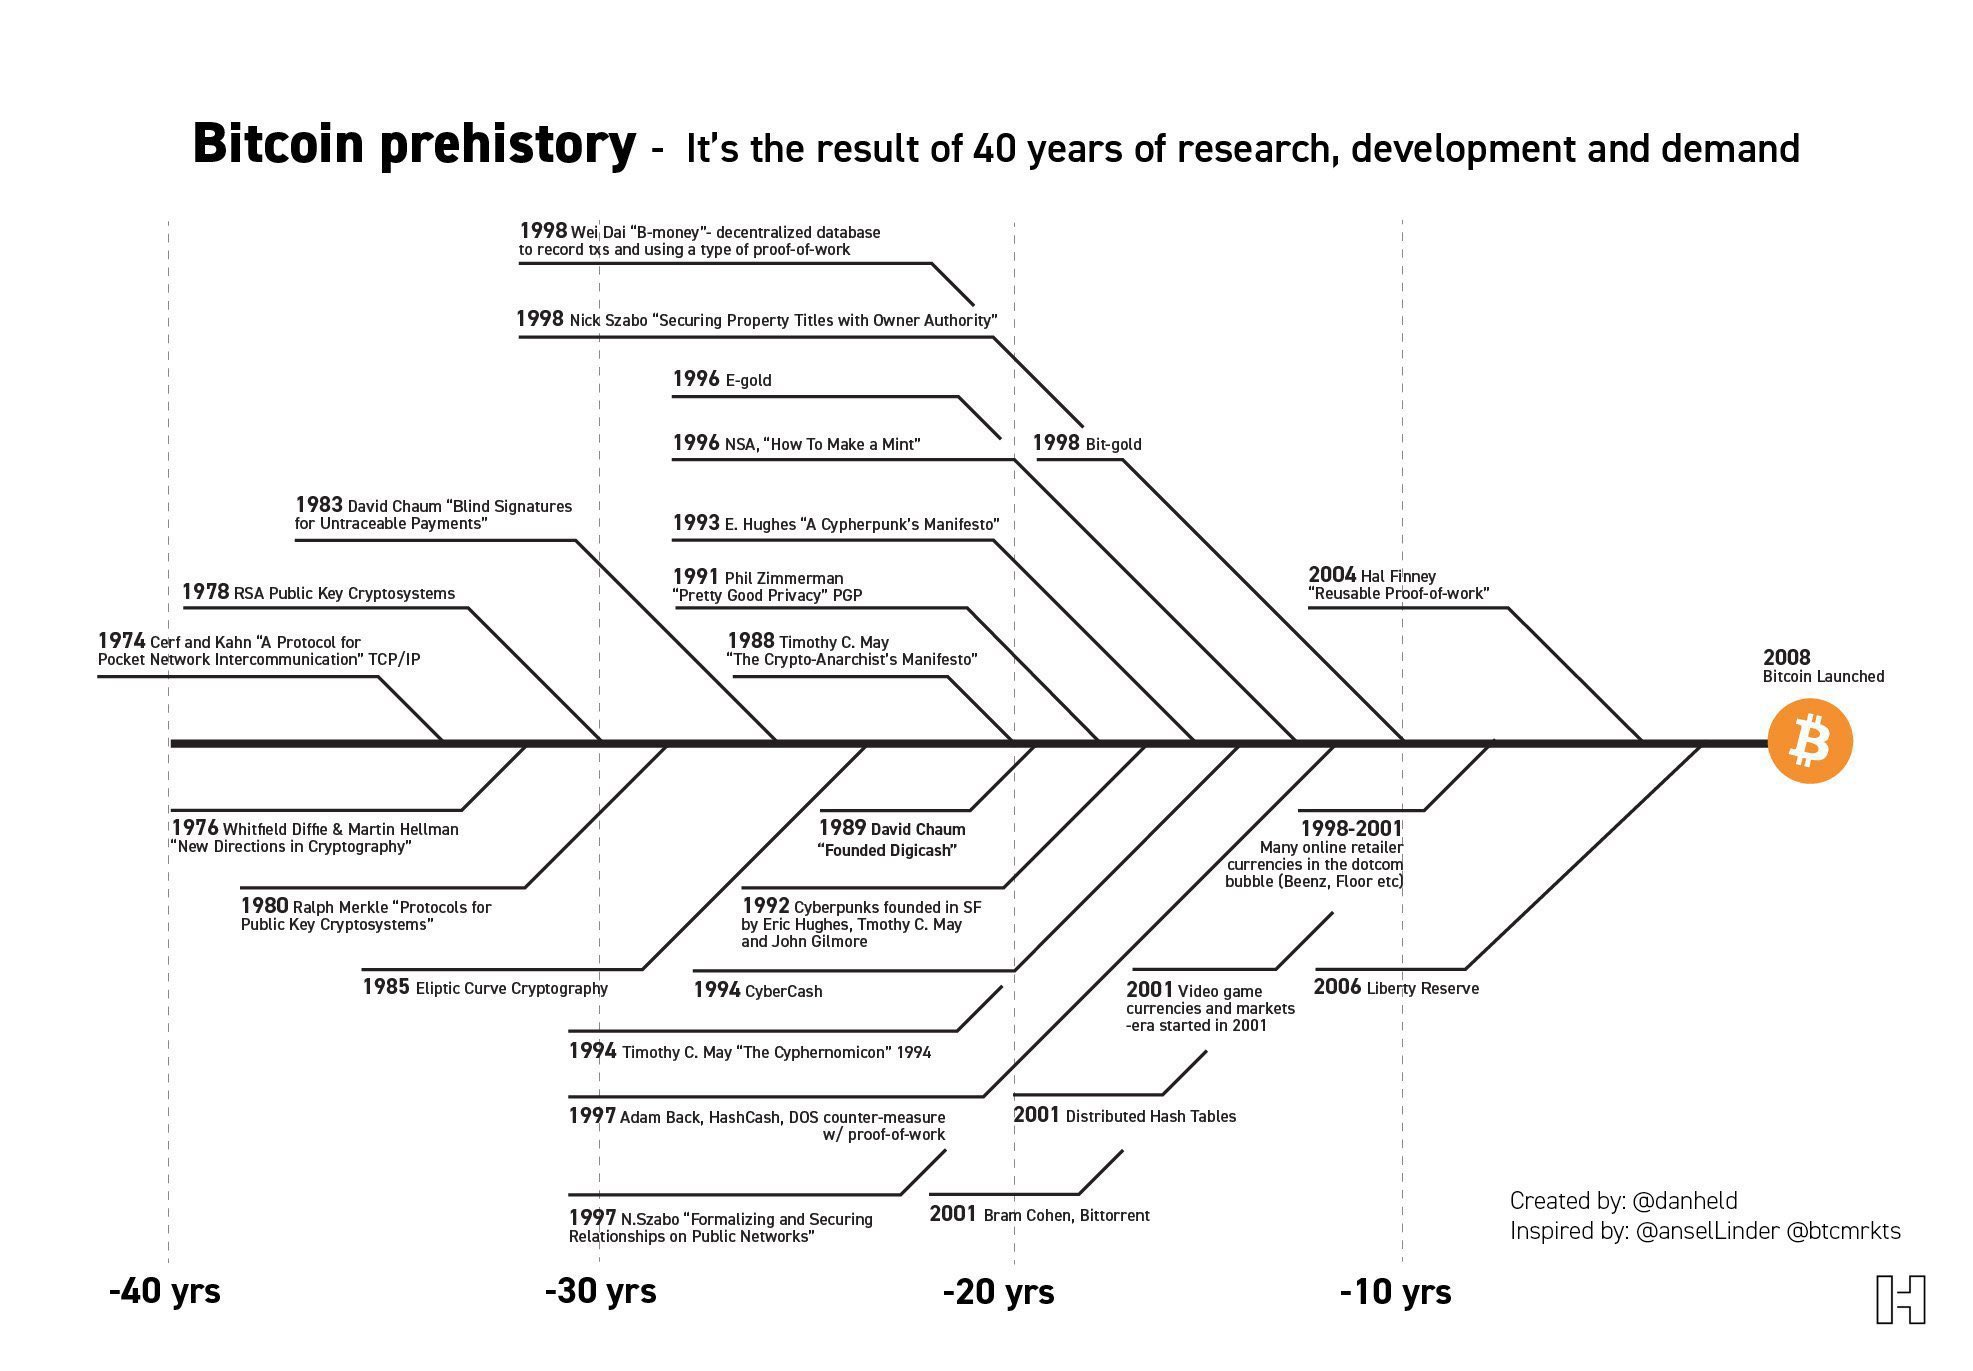
\includegraphics[width=\linewidth]{prehistory}
  \caption{Dan Held: \href{https://www.danheld.com/blog/2019/1/6/planting-bitcoinsoil-34}{Bitcoin prehistory} used with permission.}
  \label{fig:prehistory}
\end{figure}

There is enormous complexity and scope, as seen in Figure \ref{fig:venn}, and yet genuinely useful products are elusive.
\begin{figure*}[ht]\centering % Using \begin{figure*} makes the figure take up the entire width of the page
	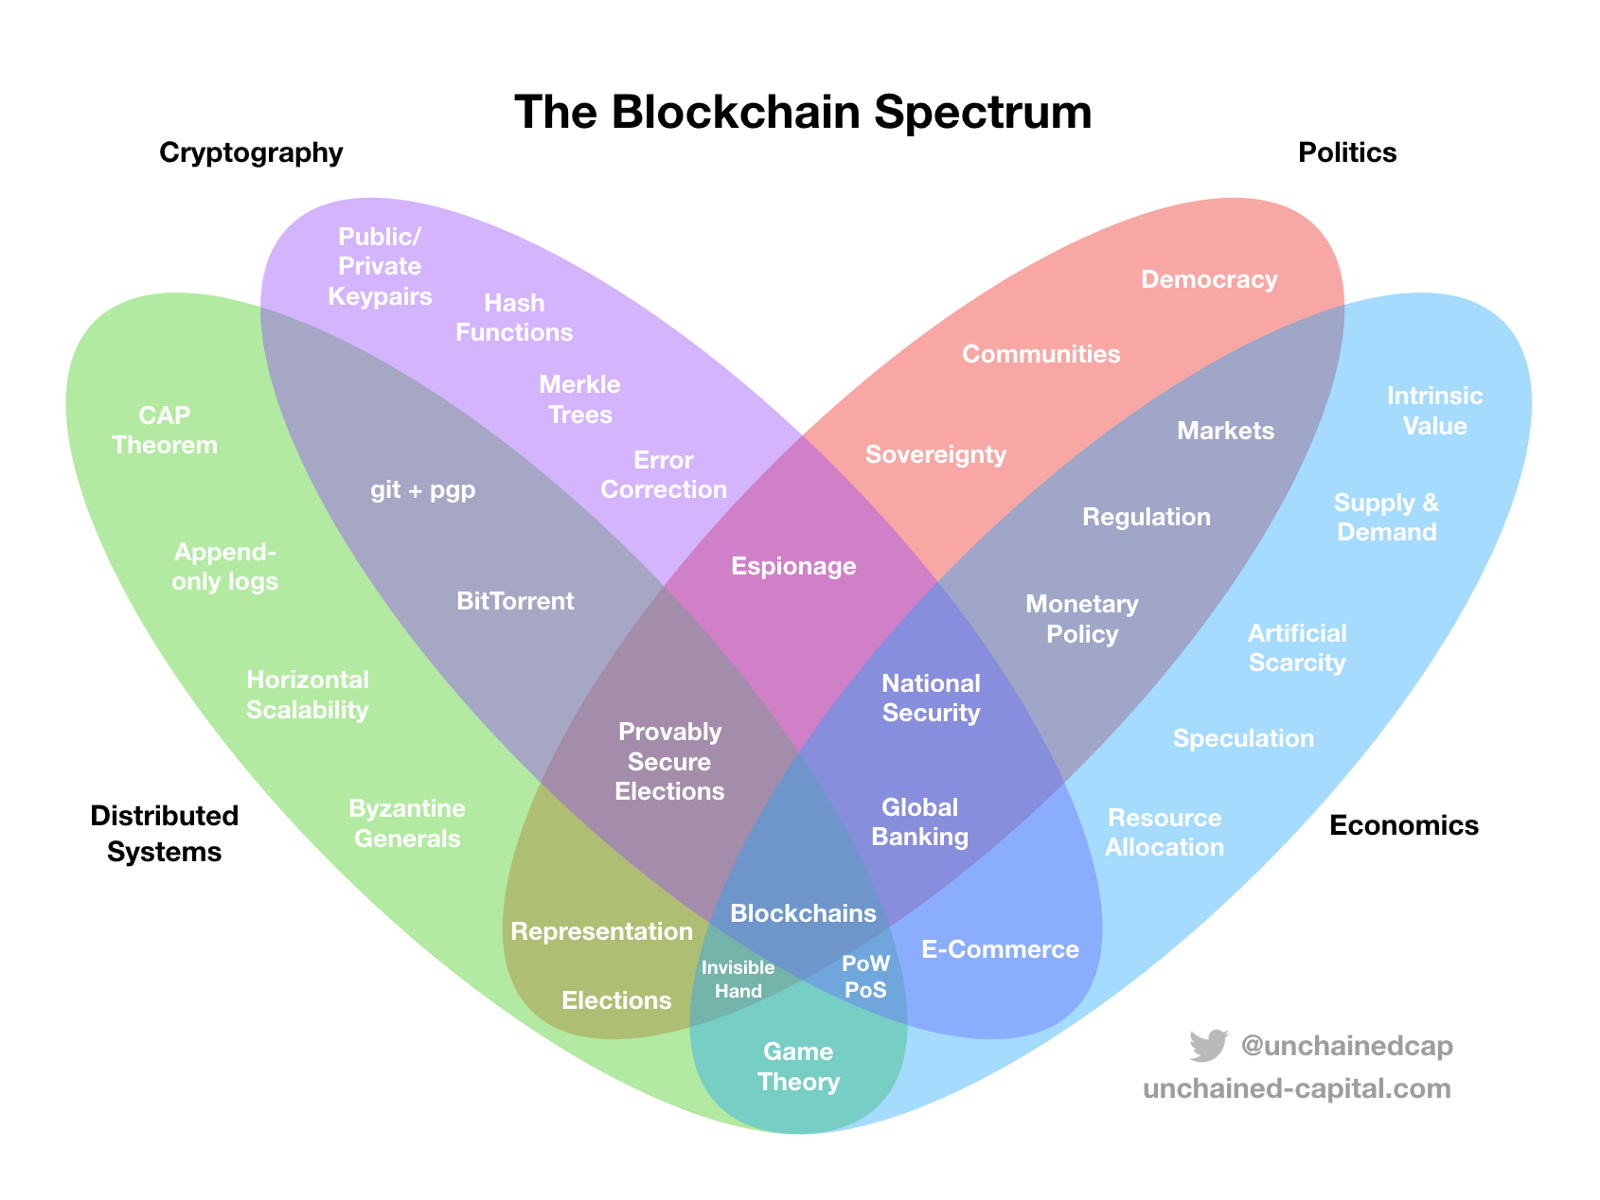
\includegraphics[width=\linewidth]{venn}
	\caption{\href{https://unchained.com/blog/blockchain-spectrum/}{Intersecting disciplines}. Reused with permission \href{https://unchained.com/}{Dhruv Bansal}}
	\label{fig:venn}
\end{figure*}
It can be argued that the whole concept of crypto/blockchain is somewhat flawed, as the vast majority of the technology offerings are not properly distributed, and "there are many scenarios where traditional databases should be used instead"\cite{casino2019systematic}.\\
It is surprising hard to pin down a simple explanation for the features which define blockchain. These ``key takeaway'' \href{https://www.investopedia.com/terms/b/blockchain.asp}{from Investopedia} are a neat summary however.\\
\begin{itemize} \item Blockchain is a specific type of database. \item It differs from a typical database in the way it stores information; blockchains store data in blocks that are then chained together. \item As new data comes in it is entered into a fresh block. Once the block is filled with data it is chained onto the previous block, which makes the data chained together in chronological order. \item Different types of information can be stored on a blockchain but the most common use so far has been as a ledger for transactions. \item In Bitcoin’s case, blockchain is used in a decentralized way so that no single person or group has control—rather, all users collectively retain control. \item Decentralized blockchains are ``append only''. In effect this means that the data entered becomes irreversible over time. For Bitcoin, this means that simple economic transactions are permanently recorded and viewable to anyone. \end{itemize}
In principle blockchains provide a differentiated trust model. With a properly distributed system blockchain can be considered ``trust minimised''. This is important for some, but not all people. In an era when data breaches and corporate financial insolvency intersect with a collapse in trust of institutions, it is perhaps useful to have an alternative model for storage of data, and value. Thanks to a natural fit with strong encryption, and innate resistance to censorship by external parties, these systems lend themselves well to `borderless' applications. Finally, a host of well engineered open source code repositories makes the cost of adoption relatively low.\\
Within DLT/blockchain there seem to be as many opinions on the value of the technology as there are implementations. There are thousands of different `chains' and many more tokens which represent value on them. A majority of these are code forks of earlier projects. Most are defunct yet still have some residual `value' locked up in them as a function of their `distributed' tokens. \\ 
Because the space is comparatively new, subject to \href{https://www.esma.europa.eu/press-news/consultations/call-evidence-dlt-pilot-regime}{scant regulation}, and often open source, it is possible to clone a github, change a few lines of code, and front it with a website in order to create `scams', and this happens very often \cite{golumbia2020cryptocurrency}.\\
The following sections give an overview of the major strands of the technology. First is Ethereum, mainly to discount it's use and get to more accessible offerings.
\section{Ethereum}
Ethereum \cite{buterin2013ethereum} is the second most secure public blockchain (\href{https://howmanyconfs.com/}{by about 50\%}), and second most valuable by \href{https://coinmarketcap.com/}{market capitalisation} (though this comparison is somewhat strained). It is the natural connection from Web3 to the rest of the paper, so it will be considered first.\\
It is touted as `programmable money'. It, unlike bitcoin, is Turing complete, able to run a \href{https://ethereum.org/en/developers/docs/evm/}{virtual machine} within the distributed network (albeit slowly), and can therefore process complex transactional contracts in the settlement of value. This has given rise to the new field of `distributed finance', or DeFi (described later), alongside many interesting trust minimised immutable ledger public database ideas. \\
There are trade-offs and problems with Ethereum (Eth/Ether) which currently increase the 'participation floor' and makes the network far less suitable for entry level business to business use. The ledger itself being a computational engine, with write only properties, is enormous. Specialist cloud hardware is required to run a full node (copy of the ledger), and partial nodes are the norm. Even partial nodes are run chiefly by one specialist cloud provider (Infura). Moreover the network is centrally controlled by its creator and the `miners'. There is a strong case to answer that Eth is \href{https://blog.mollywhite.net/blockchains-are-not-what-they-say/}{neither distributed}, nor trustless, and in fact therefore fails to be differentiated from a DLT, undermining some of it's claims.\\
With that said there are many talented developers doing interesting work on the platform, and innovation is fast paced. It is entirely normal for technology projects to launch their distributed ledger idea on and within the Ethereum network. These ``initial coin offering'' generate tradable tokens which can accrue value or demonstrate smart contract utility. Such is the level of nefarious activity on these networks that they have a poor reputation, and are difficult to audit, launch, and maintain. The overriding problem of using a blockchain for utility applications is that people can and will simply lie for criminal purpose when entering data into the ledger. It is far more likely that Ethereum is simply a speculative bubble than any of the claims for utility being born out.
\subsection{Mining and Gas}
Ethereum has a significant barrier to entry because of high fees to use the network. The system is Turing complete; able to programatically replicate any other computational system. This includes endless loops in code, so it is trivial to lock up the computational bandwidth of the while system, in a smart contract commitment, through a web wallet. To mitigate this existential `denial of service attack' the `gas' system demands that users spend some of their locked up value to operate on the network. In this way a transaction loop would quickly erode the available gas and stop looping. As the popularity of the system has grown, so too have the gas fees. It can sometimes cost hundreds of dollars to do a single transaction, though it is more normally just a few tens of dollars. This is a huge problem for potential uses of the network. It is currently a proof of work system like Bitcoin (this is described in the next section), and has a \href{https://news.trust.org/packages/cryptocurrency-and-climate/}{huge energy footprint} to secure the network. It also ties up global supply of PC graphics cards used for it's mining model, making them far more expensive.\\
\subsection{Upgrade roadmap}
Ethereum was designed from the beginning to move to a `proof of stake' model where token holders underpin network consensus through complex automated voting systems based upon their token holding. This is now called \href{https://blog.ethereum.org/2022/01/24/the-great-eth2-renaming/}{Ethereum Consensus Layer}. Like much of the rest of `crypto' the proposed changes will concentrate decisions and economic rewards in the hands of major players, early investors, and incumbents. This is a far cry from the stated aims of the technology.\\
Primarily because of the barrier to entry, we do not intend for Ethereum to be in scope as a method for value transfer within metaverses at this time.

\section{Bitcoin}   The first practical blockchain was the Bitcoin network \cite{Nakamoto2008}, some two decades after Haber et al. first described the idea \cite{haber1990time} It can be considered a triple entry book keeping system \cite{ijiri1986framework, faccia2019accounting}, the first of it's kind, integrating a `provable' timestamp with a transaction ledger. Some see this as the first major innovation in ledger technology since double entry was codified in Venice in fourteen seventy five\cite{sangster2015earliest}. \\
It was created pseudonomously in 2009 as a direct response to the perceived mishandling of the 2008 global financial crisis, with the stated aim of challenging the status quo and the \href{https://www.forbes.com/sites/peterizzo/2021/09/29/against-cryptocurrency-the-ethical-argument-for-bitcoin-maximalism/?sh=317f2c85371b}{unequal access} to opportunity it provides. The IMF has recently conceded that the Bitcoin \href{https://blogs.imf.org/2022/01/11/crypto-prices-move-more-in-sync-with-stocks-posing-new-risks/}{poses a risk} to the traditional financial systems, so it could be argued that it is succeeding in this original aim.
The \href{https://en.bitcoin.it/wiki/Genesis_block}{``genesis block''} which was hard coded at the beginning of the `chain' contains text from The Times newpaper detailing the second bank bailout.\\ 
Satoshi Nakamoto (the name of the publishing entity) \href{https://bitcoinmagazine.com/technical/what-happened-when-bitcoin-creator-satoshi-nakamoto-disappeared}{disappeared from the forums} forever in 2010.\\
Although there were some earlier experiments (hashcash, b-money etc), Bitcoin is the first viably decentralised `cryptocurrency'; the network is used to \href{https://www.aier.org/article/why-does-bitcoin-have-value/}{store economic value} because it is judged to be secure and trusted. It is a singular event in that it became established at scale, such that it could be seen to be a fully distributed system, without a controlling entity. This is the differentiated trust model previously mentioned. This relative security is the specific unique selling point of the network. It is many times more secure than all the networks which came after based on a like for like comparison of \href{https://howmanyconfs.com/}{transaction `confirmations'}. This network effect of Bitcoin is a compounding feature, attracting value through the security of the system. It is deliberately more conservative and feature poor, preferring instead to \href{https://bips.xyz/}{add to it's feature set} slowly, preserving the integrity of the value invested in it over the last decade. At time of writing it is a \href{https://fiatmarketcap.com/}{top quartile} largest global currency and has settled over \$12 trillion Dollars in 2021, though Makarov et al. contest this, citing network overheads, and speculation \cite{makarov2021blockchain}. Institution grade `exchange tradable funds' which allow investment in Bitcoin are available throughout the world, and the native asset can be bought by the public easily through apps in all but a handful of countries as seen in Figure \ref{fig:settled2021}. 
\begin{figure}
  \centering
    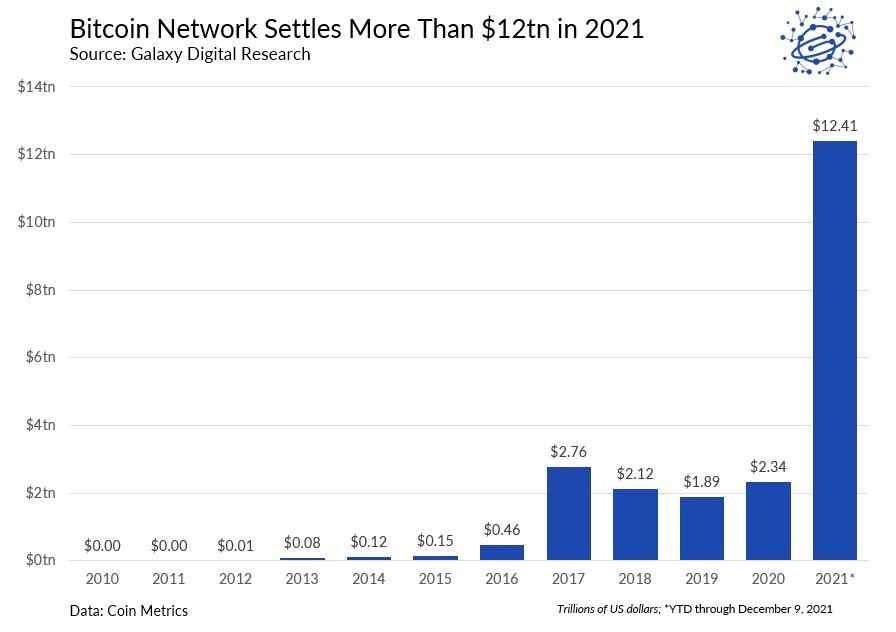
\includegraphics[width=\linewidth]{settlement2021}
  \caption{\href{https://twitter.com/glxyresearch/status/1469039427028664320?}{Growth in settlement} value on the Bitcoin network.}
  \label{fig:settled2021}
\end{figure}
Only around 7 transactions per second can be settled on Bitcoin. The native protocol does not scale well, and moreover this in an inherent trade-off as described by Croman et al. in their positioning paper on public blockchains \cite{croman2016scaling}. Over time competition for the limited transaction bandwidth drives up the price to use the network. This effectively prices out small transactions, even locking up some value below what is a termed the '\href{https://github.com/bitcoin/bitcoin/blob/v0.10.0rc3/src/primitives/transaction.h#L137}{dust limit}' of unspent transactions too small ever to move again \cite{delgado2018analysis}. \\
Bitcoin has developed quickly, with a \href{https://phemex.com/blogs/crypto-bitcoin-s-curve-adoption-curve}{faster adoption} than even the internet itself. It is now a mature ecosystem, and is seeing adoption as a \href{https://bitcointreasuries.net/}{corporate treasury asset}. \\
Adoption by civil authorities is increasing, and legislators the world over are being forced to \href{https://www.politico.com/news/2022/01/16/bitcoin-crashes-the-midterms-527126}{adopt a position}. Many city treasuries have added it to their balance sheet, and it is legal tender in the country of El Salvador\cite{oxford2021salvador}, and this will be explored more later. Global asset manager ``Fidelity'' wrote the following in their \href{https://www.fidelitydigitalassets.com/articles/2021-trends-impact}{2021 trends report}.\\
``We also think there is very high stakes game theory at play here, whereby if bitcoin adoption increases, the countries that secure some bitcoin today will be better off competitively than their peers. Therefore, even if other countries do not believe in the investment thesis or adoption of bitcoin, they will be forced to acquire some as a form of insurance. In other words, a small cost can be paid today as a hedge compared to a potentially much larger cost years in the future. We therefore wouldn't be surprised to see other sovereign nation states acquire bitcoin in 2022 and perhaps even see a central bank make an acquisition.''\\

\subsection{The Bitcoin Network Software}
There isn't a single github which can be considered the final arbiter of the development direction, because it is a distributed community effort with some \href{https://decrypt.co/66740/who-are-the-fastest-growing-developer-communities-in-crypto}{400 developers} out of a wider `crypto' pool of around 9000 contributors. \href{https://bitcoinops.org/en/newsletters/2021/12/22/}{Development and innovation continues} but there is an empahasis on careful iteration to avoid damage to the network. Visualisation of code commitments to the various open source software repositories can be seen at \href{https://www.youtube.com/channel/UC4DT4qudqogkmbqVAQy8eFg/videos}{Bitpaint youtube channel} and in Figure \ref{fig:gource}.\\

\begin{figure*}[ht]\centering % Using \begin{figure*} makes the figure take up the entire width of the page
	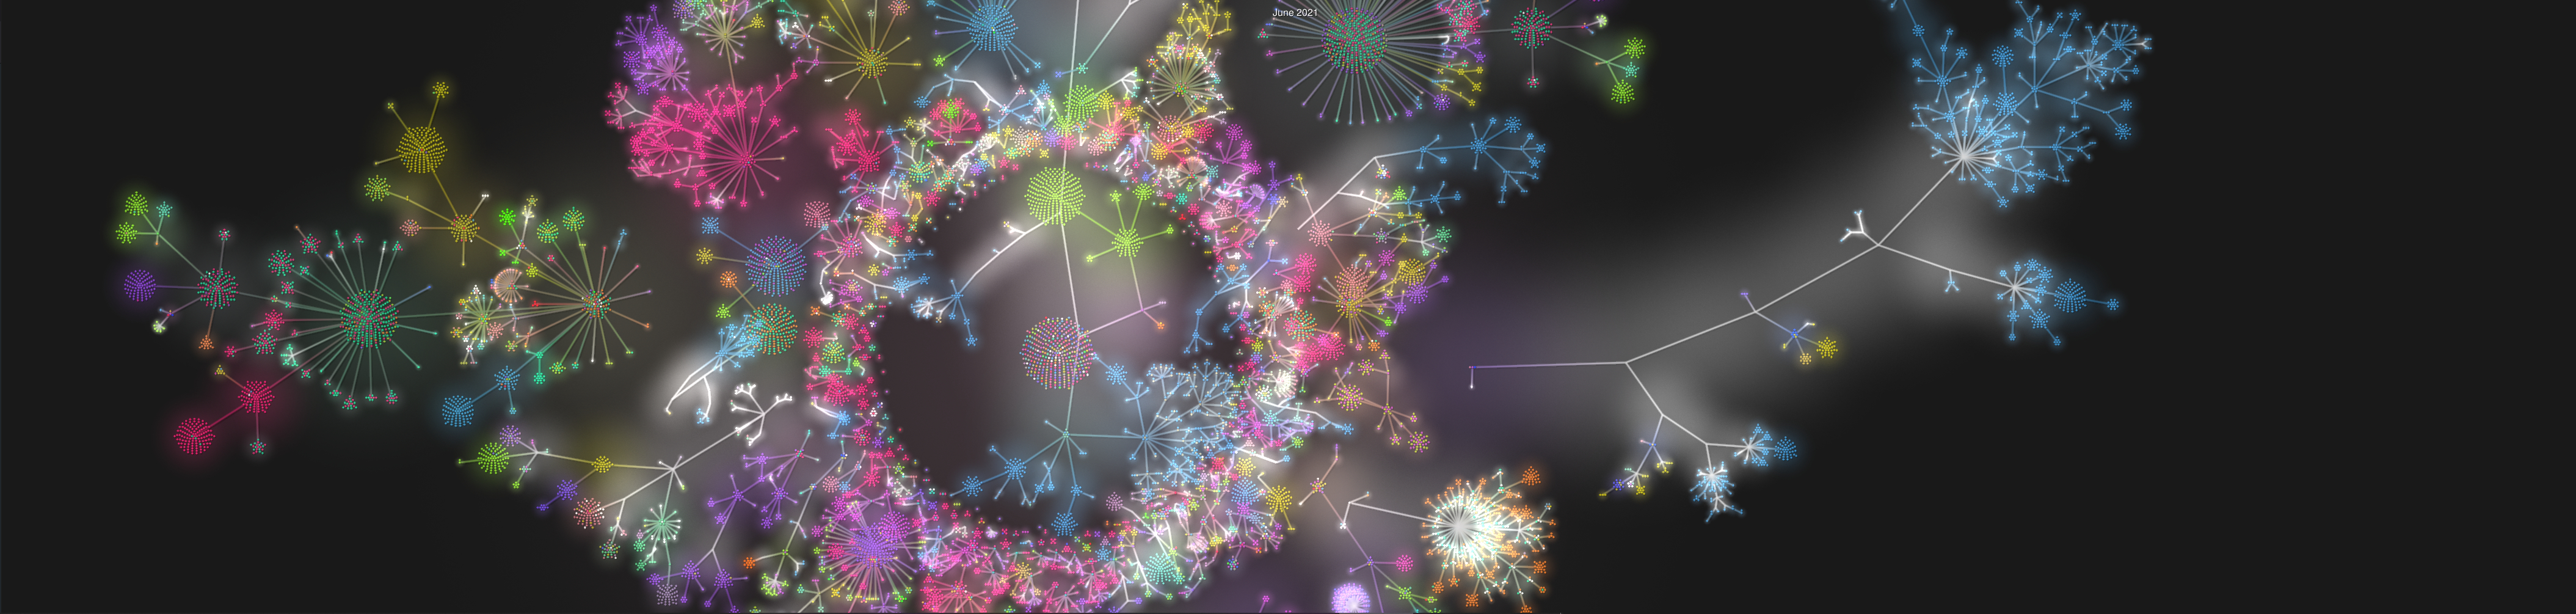
\includegraphics[width=\linewidth]{gource}
	\caption{\href{https://github.com/bitpaint/bitcoin-gources}{Bitpaint}: Contributions to the Bitcoin ecosystem. Reused with permission.}
	\label{fig:gource}
\end{figure*}

\href{https://github.com/bitcoin/}{Bitcoin core} is the main historical effort, but there are alternatives (\href{https://github.com/libbitcoin/libbitcoin-node/wiki}{LibBitcoin in C++}, \href{https://github.com/btcsuite/btcd}{BTCD in Go}, and \href{https://bitcoinj.github.io/getting-started}{BitcoinJ in Java}). 
\subsection{Mining and Energy concerns}
Bitcoin uses a staggering amount of energy to secure the blockchain, and this \href{https://www.edmundconway.com/bitcoin-money-and-the-planet/}{has climate repercussions}. It is an industrial scale global business with `mining companies' investing \href{https://ir.marathondh.com/news-events/press-releases/detail/1272/marathon-digital-holdings-bitcoin-mining-fleet-to-reach}{hundreds of millions of pounds} at a time \href{https://www.tomshardware.com/news/intel-to-unveil-bitcoin-mining-bonanza-mine-asic-at-chip-conference}{specialist ASIC mining hardware and facilities}. This is Adam Back's ``proof of work'',  and is essential to the technology. \href{https://ccaf.io/cbeci/index}{The Cambridge Bitcoin Energy Consumption Index} monitors this energy usage.\\
Such businesses can mine a Bitcoin for around \$5k-\$10k per coin, so the profit margins \href{https://www.nicehash.com/profitability-calculator}{are considerable} (based on 30-40 Joule/terahash and power rate less than 5 cents /kilowatt hour and excluding hardware costs). This is not to say that all mining is, or should be, so concentrated. Anyone running the hashing algorithm can \href{https://twitter.com/ckpooldev/status/1485585814419812356}{get lucky} and claim the block reward. PoW ties the value of the `money' component of Bitcoin directly to energy production. This is not a new idea as can be seen in Figure \ref{fig:energyNYT}. Henry Ford proposed an intimate tie between energy and money to create a separation of powers from government.\
\begin{figure}
  \centering
    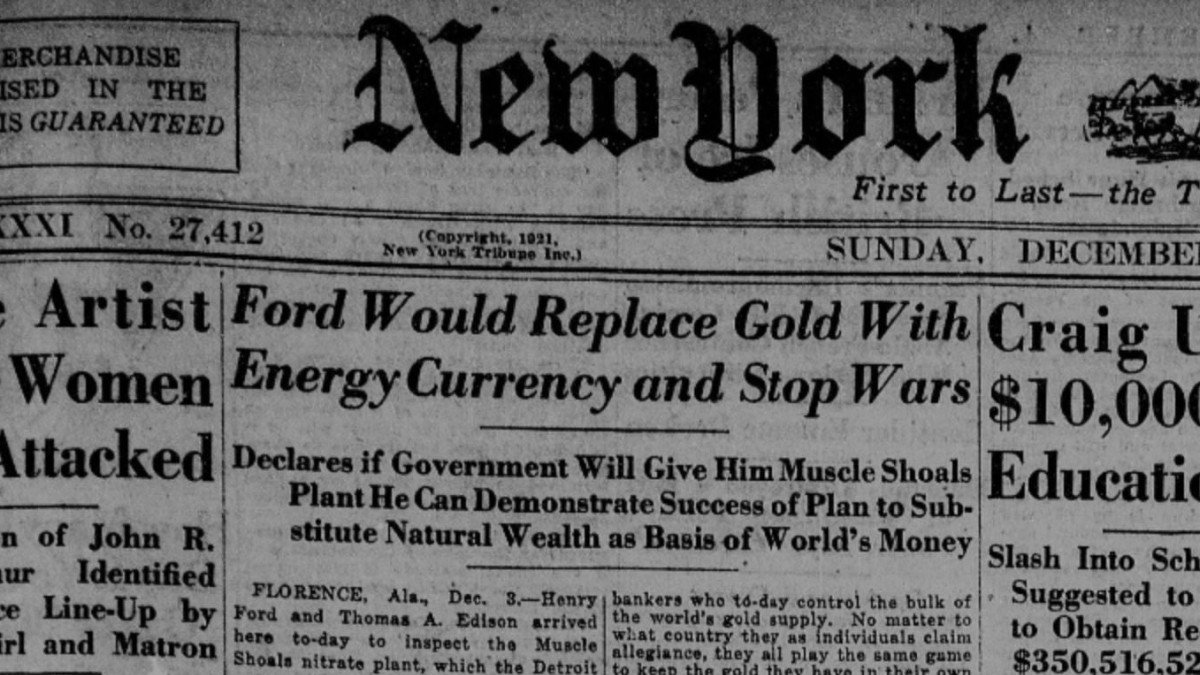
\includegraphics[width=\linewidth]{energyNYT}
  \caption{\href{https://www.nytimes.com/1921/12/06/archives/mr-fords-energy-dollar.html}{Intimate tie between energy and money, Henry Ford}}
  \label{fig:energyNYT}
\end{figure}

The potential ecological footprint of the network has always been a concern; Hal Finney himself was \href{https://twitter.com/halfin/status/1153096538}{thinking about this issue} with a mature Bitcoin network as early as 2009. \\
Proponents of the technology say that the balance shifted dramatically in 2021 with China outright banning the technology; this has forced the bulk of the energy use away from `dirty coal' as seen in Figure \ref{fig:miningshare}. Some analysts \href{https://docs.google.com/document/d/1N2N-5jY00cmteoY_puWI9oosM1foa4EQqsO1FFfIFR4/edit}{propose mitigations}, or even suggest that \href{https://medium.com/@magusperivallon/a-financial-hail-mary-for-the-climate-an-argument-for-bitcoin-adoption-9c58e707d0}{`ending financialisation' through use of Bitcoin} may be net positive for the environment. Recently for example Baur and Oll found that \textit{``Bitcoin investments can be less carbon intensive than standard equity investments and thus reduce the total carbon footprint of a portfolio.''}\cite{baur2021bitcoin}. 

\begin{figure}
  \centering
    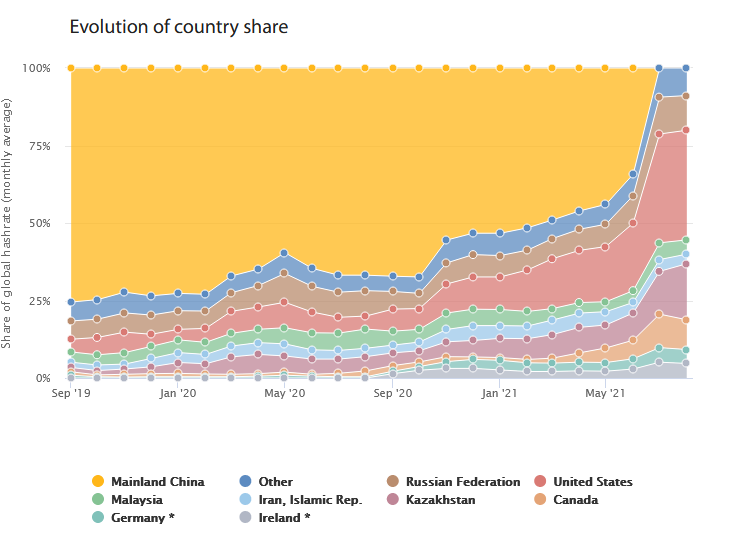
\includegraphics[width=\linewidth]{miningshare}
  \caption{Hash rate \href{https://ccaf.io/cbeci/ining_map}{suddenly migrates} from China [Reuse rights requested]}
  \label{fig:miningshare}
\end{figure}

The power commitment to the network is variously projected \href{https://www.nature.com/articles/s41558-018-0321-8}{to increase}, or \href{https://assets.website-files.com/614e11526f6630959fc98679/616df63a27a7ec339f5e6a80_NYDIG-BitcoinNetZero_SML.pdf}{level off over time}, but certainly not decrease. The industry now argue that economic pressures mean that most of the `hashrate' is \href{https://bitcoinminingcouncil.com/q4-bitcoin-mining-council-survey-confirms-sustainable-power-mix-and-technological-efficiency/}{generated by renewable energy}\cite{blandin20203rd}. Certainly there is growing interest and adoption of so called ``stranded energy mining''  which cannot be effectively transmitted to consumers, and is thereby sold at a huge discount while also \href{https://www.renewableenergyworld.com/wind-power/900mw-wind-farm-to-power-bitcoin-mining-operation/}{developing power capacity} \cite{bastian2021hedging}. The most cited example of this is El Salvador's `volcano mining' which is supporting their national power infrastructure plans. A more poignant example is the \href{https://www.timesunion.com/news/article/Mechanicville-hydro-plant-gets-new-life-16299115.php}{Mechanicville hydro plant in the USA}. The refurbishment of this 123 year old power plant is being funded by Bitcoin mining. This is the \href{https://www.lynalden.com/bitcoin-energy/}{``buyer of last resort''} model first \href{https://squareup.com/us/en/press/bcei-white-paper}{advanced by Square Inc}. Critics highlight the potential \href{https://www.fitchratings.com/research/us-public-finance/crypto-mining-poses-challenges-to-public-power-utilities-24-01-2022}{impact of mining on local energy} prices\cite{benetton2021cryptomining}. \href{https://www.youtube.com/watch?v=6LP8G-oZnEs}{The debate} whether this consumption is `worth' it is complex and \href{https://www.aei.org/technology-and-innovation/no-hearing-on-bitcoins-energy-use-is-complete-without-nic-carter/}{rapidly evolving}. Is a trillion dollar asset which \href{https://www.theheldreport.com/p/bitcoin-vs-gold}{potentially replaces the money utility of gold}, but doesn't need to be stored under guard in vaults (Figure \ref{fig:goldmanVgold}), worth the equivalent power consumption of clothes dryers in North America? Probably not with the current level of adoption, but this is an experiment in replacing global money. This paper offers no firm opinion.
\begin{figure}
  \centering
    \includegraphics[width=\linewidth]{goldmanvgold}
  \caption{Goldman suggest growth opportunity and potential demonetisation of gold?}
  \label{fig:goldmanVgold}
\end{figure}
\subsection{Bitcoin nodes }
The Bitcoin network can be considered a triumvirate of economic actors, each with different incentives. These are:
\begin{itemize}
\item Holders and users of the tokens, including exchanges and market makers, who make money speculating, arbitraging, and providing liquidity into the network.
\item Miners, who profit from creation of new UTXOs, and receive payments for adding transactions to the chain. In return they secure the network.
\item Node operators, who enforce the consensus ruleset which the miners must abide by in order to propagate new transaction into the network. In return node operators optimise their trust minimisation, and help protect ths network from changes which might undermine their speculation and use of the tokens.
\end{itemize}
There are currently around \href{https://bitnodes.io/}{15,000 bitcoin nodes} distributed across the world. 
Since and IT engineer \href{https://stadicus.com/}{Stadicus} released his \href{https://raspibolt.org/backstory.html}{Raspibolt guide} in 2017 there has been an explosion of small scale Bitcoin and Lightning node operators. 
Around thirty thousand Raspberry Pi Lighting nodes (which are also by definition bitcoin nodes) run one of the following \href{https://github.com/bavarianledger/bitcoin-nodes}{open source distributions}, with the most noteworth explained alongside their standout featureset:
\begin{itemize}
\item \href{https://github.com/rootzoll/raspiblitz}{Raspiblitz} offers fully opensource lightning focused functionality with a touchscreen display
\item \href{https://github.com/mynodebtc/mynode}{Mynode} focuses on easy of use through a web interface and has many modules which users can try out.
\item \href{https://github.com/getumbrel/umbrel-os}{Umbrel} is a more user friendly multi purpose node allowing access to a suite of Bitcoin and self sovereign individual tools.
\item \href{https://wiki.ronindojo.io/}{RoninDojo} is designed for use alongside the privacy focused \href{https://samouraiwallet.com/}{Samourai mobile wallet}.
\item \href{https://github.com/fort-nix/nix-bitcoin}{Nix bitcoin} focuses on security of the underlying operating system by building on  NixOS.
\item \href{https://nodl.it}{NODL} is a premium prebuilt node focusing on security of the more performant hardware, and underlying operating system. It offers additional privacy tools.
\item \href{https://store.start9labs.com/collections/embassy}{Start9 Embassy} is a small form factor prebuilt unit at a lower price. It is a venture capital funded project with a more restrictive license but offers a suite of easy to use self sovereignty tools including Bitcoin. 
\end{itemize}

Rather than using one of these distributions we plan to support a new metaverse focused suite of these tools based around the nix distribution.
\href{https://nydig.com/research/nydig-bitcoin-101}{Consider  mining the NYDIG primer for information}

%Feedback from James this is a completely fair solution to the byzantine general problem of distributed consensus i will write this into the paper, it's not there and it should be that proof or work, combined with a couple of other novelish features from elsewhere in history nakamoto consensus, which is the basis of the whole technology without it there is a zero cost to attacking the network with it it's virtually impossible to attack it meaningfully there's suspected to be around 4M bitcoin lost forever 18M are mined I think, so that's around 14M in the wild, each subdivided by 100M to give sats, each of which can currently be subdivided again by 1000. interestingly that's quite changeable. more zeros could be added. the point is the cap is unchangeable unless you can find a way to switch the software on 75,000 secret home nodes against their financial interest githubs are referencable if I like I think What happens when the last coin is mined? Isn’t the mining itself something to do with validating transactions? Who does that after there are no more to mine? there's no rules to an unlicense license What happens when the last coin is mined? Isn’t the mining itself something to do with validating transactions? Who does that after there are no more to mine? it's a big known unknown the theory is that the fees will rise as the use rises, and the miners will benefit from the fees not the mining both of which are decent rewards if miners think it's not worth it then they drop out and the network adjusts the difficulty automatically every 2 weeks to compensate those who remain with more reward so in principle it sorts itself out but nobody is sure and there's no way to test it this is excellent, I will make all this clear, thanks a great help!

\subsection{Upgrade roadmap}
Taproot\\
\href{https://utxos.org/}{BIP-119}
\subsection{Risks}
\begin{itemize}
\item The block reward is reduced every 4 years (epochs). This means a portion of the mining reward is trending to zero, and nobody knows what effect this will have on the incentives for securing the network through proof of work.
\item Stablecoins are a vital transitional technology (described later) but do not meaningfully exist yet on the Bitcoin network. This may change.
\item Bitcoin lacks privacy by design. All transactions are publicly viewable. This is a major drag to the concept of BTC as a money.
\item The Lightning network (described later) has terrible UX design at this time. 
\item The basic `usability' of the network is still poor in the main. Any problems which users experience demand a steep learning curve and risk loss of funds. There is obviously no tech support number people can call. 
\item Only around one billion unspent transactions can be generated a year on the network. This means that it might become impossible for everyone on the planet to have own their own Bitcoin address (with it's associated underpinning UTXO).  
\end{itemize} 

\section{Extending the BTC ecosystem }
The following section are by no means an exhaustive view of development on the Bitcoin network, but it does highlight some potentially useful ideas for supporting metaverse interactions in a useful timeframe.
\subsection{Block \& SpiralBTC}
Block (formally the payment processor ``Square'' is now an umbrella company for several smaller 'building block' companies, all of which are major players in the space. \\
SpiralBTC, formally `Square Crypto' (a subsidiary of Square) is funding development in Bitcoin and Lightning. Their main internal product is the \href{https://spiral.xyz/blog/what-were-building-lightning-development-kit/}{Lightning Development Kit} (LDK). This promising open source library and API will allow developer to add lightning functionality to apps and wallets. It is a useful contender for our metaverse applications. They also fund external open source development.\\
\subsection{BTCPayServer}
BTCPayServer is one of the recipients of a Spiral grant. It is a self hosted Bitcoin and Lightning payment processor system which allows merchants, online, and physical stores and businesses to integrate Bitcoin into their accounting systems.


\href{https://twitter.com/BtcpayServer/status/1476572743626035200}{check the roadmap}
\lipsum[50]


\section{Lightning (Layer 2)}
Lightning was a 2016 proposal by Poon and Dryja \cite{poon2016bitcoin}, and is a community driven liquidity pool which enables scaling and speed improvements for the Bitcoin network. It is mainly `powered' by \href{https://plebnet.wiki/wiki/Main_Page}{thousands of volunteers} who invest in hardware and lock up their Bitcoin in their nodes, to facilitate peer to peer transactions. Zebka et al. found that although the network is ``fairly decentralised'' it is more recently skewing to larger more established nodes \cite{zabka2022short}. Though this is a grassroots technology the nature of the design means it can likely be trusted for small scale commercial applications.\\
The following text is from \href{https://medium.com/@johncantrell97?p=5cc72f2c664}{John Cantrell}, an engineer who works on Lightning.\\
\textit{``The Lightning Network is a p2p network of payment channels. A payment channel is a contract between two people where they commit funds using a single onchain tx.  Once the funds are committed they can make an unlimited amount of instant \& free payments over the channel.
You can think of it as a tab where each person tracks how much money they are owed.  Each time a payment is made over the channel both parties update their record of how much money each person has.  These updates all happen off-chain and only the parties involved know about them. When it`s time to settle up the two parties can take the final balances of the channel and create a channel closing transaction that will be broadcast on chain.  This closing transaction sends each party the final amounts they are owed. This means for the cost of two on-chain transactions (the opening and closing of the channel) two parties can transact an unlimited number of times and the overall cost of each transaction approaches zero with every additional transaction they make over the channel. Payment channels are a great solution for two parties to transact quickly and cheaply but what if we want to be able to send money to anyone in the world quickly and cheaply?  This is where the Lightning Network comes into play, it`s a p2p network of these payment channels. This means if Alice has a payment channel with Bob and Bob has a channel with Charlie that Alice can send a payment to Charlie with Bob`s help. This idea can be extended such that you can route a payment over an arbitrary number of channels until you can reach the entire world. Routing a payment over multiple channels uses a specific contract called a Hash Time Locked Contract (HTLC).  It introduces the ability for Bob and any other nodes you route through to charge a small fee.  These fees are typically orders of magnitude smaller than onchain fees. This all sounds great but what if someone tries to cheat? I thought the whole point of Bitcoin was that we no longer had to trust anyone and it sure sounds like there must be some trust in our channel partners to use the Lightning Network? The contracts used in Lightning are built to prevent fraud while requiring no trust.  There is a built-in penalty mechanism where if someone tries to cheat and is caught then they lose all of their money.  This does mean you need to be monitoring the chain for fraud attempts.''}

%\href{https://twitter.com/marcrjandrew/status/1478052587387568130}{Five facts about lightning}
Lightning is a key scaling innovation in the bitcoin network at this time. It is seeing rapid development and adoption (Figure \ref{fig:lightningAdoption}). The popular payment app ``Cash App'' integrates the technology, and `Lightning Strike' services the USA, El Salvador, and Argentina with zero exchange and tranmission fees.

\begin{figure}
  \centering
    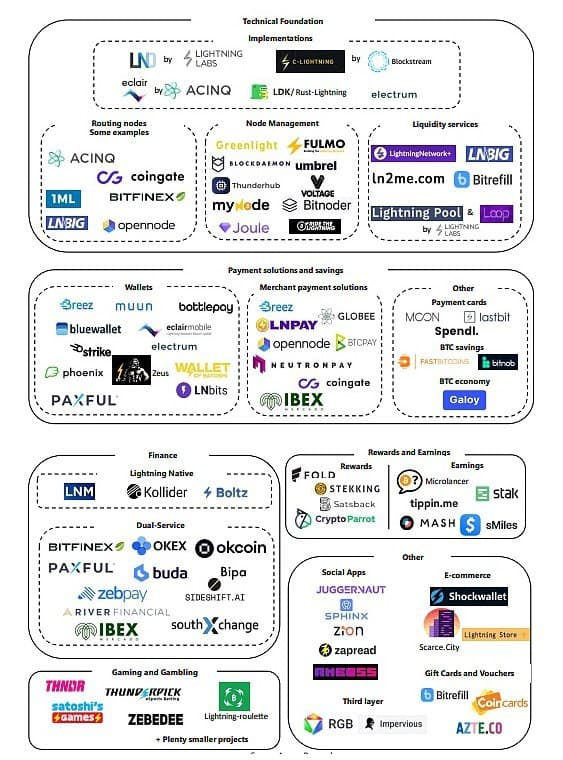
\includegraphics[width=\linewidth]{lightningAdoption}
  \caption{\href{https://www.research.arcane.no/the-state-of-lightning}{Arcane research lightning adoption overview}.}
  \label{fig:lightningAdoption}
\end{figure}
It allows for unbound scaling of transactions (millions of transations per second compared for instance to around 45,000 TPS in the VISA settlement network). Transaction costs are incredibly low, and the transaction speed virtually instantaneous.\\
The main Lightning network git is the Daemon \href{https://github.com/lightningnetwork/lnd#readme}{here} but it's worth knowing that Lighting itself really needs access to both a Bitcoin full node, and the Tor private network layer. Both Donner Labs and Zebedee have code packages which allow interaction with the lightning network within Unity. In all likelihood users would have to run a lightning / Bitcoin node and have their users interact with it. This would allow instantaneous transactions of Satoshis (the Bitcoin unit of account) between users. It would not resolve how to move money into Bitcoin or lightning. This could be handled through a web store (BTCPay Server). This is another overhead which would need weighing but opens the door to real value transacting at scale and with high security. \\
Setting up and running a lightning node is even more difficult. It is recommended to buy a \href{https://lightninginabox.co/product/1-month-btcpayserver-hosting-lightning-included/}{third party hosted} BTC / Lightning / BTCPayserver stack. 
\subsection{Micropayments}
Possibly the most important affordance of the Lightning network is the concept of micropayments, and streaming micropayments. It is very simple to transfer even \href{https://satsymbol.com/}{one satoshi} on Lightning, which is one hundred millionth of a bitcoin, and a small fraction of a penny. This can be a single payment, for a very small goods or service, or a recurring payment on any cadence. This enables streaming payments for any service, or for remittance, or remuneration. These use cases likely have enormous consequences which are just beginning to be explored. Integration of this capability into metaverse applications will be explored later.

\subsection{LNBits}
LNBits is an open source, extensible, Lightning `source' management suite. It is self hosted, and can connect to a variety of Lightning wallets, further abstracting the liquidity to provide additional functionality to network users. Remember that all of these tools run without a third party, on a £200 setup, hosted at home or within a business. The best way to explore this is to describe \textit{some} of the plugins. 
\begin{itemize}
\item ``\href{https://github.com/lnbits/lnbits-legend#lnbits-v03-beta-free-and-open-source-lightning-network-walletaccounts-system}{Accounts System}; Create multiple accounts/wallets. Run for yourself, friends/family, or the whole world!''
\item \href{https://github.com/lnbits/lnbits-legend/tree/quart/lnbits/extensions/events#events}{Events plugin} allows QR code tickets to be created for an event, and for payments to be taken for the tickets.
\item \href{https://github.com/lnbits/lnbits-legend/tree/quart/lnbits/extensions/jukebox#jukebox}{Jukebox} creates a Spotify based jukebox which can be deployed online or in physical locations.
\item \href{https://github.com/lnbits/lnbits-legend/tree/quart/lnbits/extensions/livestream#dj-livestream}{Livestream} provides an interface for online live DJ sets to receive real-time Lightning tips, which can be split automatically in real-time with the music producer.
\item \href{https://github.com/lnbits/lnbits-legend/tree/quart/lnbits/extensions/tpos#tpos}{TPoS}, \href{https://github.com/arcbtc/LNURLPoS#lnurlpos}{LNURLPoS} \& \href{https://github.com/lnbits/lnbits-legend/tree/quart/lnbits/extensions/watchonly#watch-only-wallet}{OfflineShop} support online \href{https://rapaygo.com/}{and offline} point of sale (Figure \ref{fig:LnBitsPoS}).
\item \href{https://github.com/lnbits/lnbits-legend/tree/quart/lnbits/extensions/paywall#paywall}{Paywall} creates web access control for content. 
\item \href{https://github.com/LightningTipBot/LightningTipBot#lightningtipbot-}{LightningTipBot} is a custodial Lightning wallet and tip handling bot within the popular on Telegram instant messenger service.
\end{itemize}
\begin{figure}
  \centering
    \includegraphics[width=\linewidth]{LnBitsPoS}
  \caption{One of the many \href{https://nl.aliexpress.com/item/1005003589706292.html}{prebuilt} and \href{https://github.com/arcbtc/LNURLPoS}{kit} options for Lightning `point of sale'}
  \label{fig:LnBitsPoS}
\end{figure}
Together these plugins are incredibly useful primitives which are likely to be translatable to a multi party metaverse application. A proposal for building a more specific plugin along these lines is detailed later.
\subsection{Etleneum}
Etleneum is a centralised smart contract platform built around Lightning invoices. It is most notable as a sign of things to come. There are \href{https://etleneum.com/#/contracts}{many small contracts} available to try on the site, such as a \href{https://etleneum.com/#/contract/c8w0c13v75}{simple market} for moving value between lightning and Bitcoin layer 1, or this \href{https://simple-auction.etleneum.com/}{simple auction}.  Contracts are able to operate on data drawn from the wider web, and automatically send and receive lightning payments based on conditional states. It should be viewed as an experiment which allows tinkering in smart contracts, and therefore potentially useful for the software proposed in the final section.
\subsection{Message passing}
\lipsum[50]
\section{Liquid federation (layer 2)}
``Federation members contribute to the Liquid Network's security, gain voting rights in the board election and membership process, and provide valuable input on the development of new features. Members also benefit from the ability to perform a peg-out without a third party, allowing their users to convert between L-BTC and BTC seamlessly within their platform.''\\

\href{https://bitcoinmagazine.com/business/bitcoin-liquid-network-gains-six-new-federation-members}{Now 63 members}

Bitmatrix, Digital Markets (DIGTL), GMO Coin, Mempool, Specter, and Zaprite are now part of the 63-member group.

\href{https://bitcoinmagazine.com/markets/el-salvador-president-nayib-bukele-samson-mow-volcano-bitcoin-bond}{El Salvador volcano bonds stuff}
\lipsum[50]

\section{Bitcoin Layer 3}
Increasingly important features of modern blockchain implementations are programmability through smart contracts, and issuance of arbitrary tokens. Assigning a transaction to represent another thing like an economic unit, energy unit, or real world object, and operating on those abstractions within the chain logic. Chief among these use cases are stablecoins such as Tether, which are pegged to national currencies and described in the next section. Bitcoin has always supported very limited contracts called scripts, and stablecoin issuance has existed in Bitcoin since 
\href{https://www.omnilayer.org/}{Omni Layer}. Omni was the first issuer of Tether, but more recently these important features have passed to other layer one chains. This year is likely to see the \href{https://www.hiro.so/blog/bitcoin-ecosystem-a-guide-to-programming-languages-for-bitcoin-smart-contracts}{resurgence of this capability} on Bitcoin, which of course benefits from a better security model. In order to properly understand the use of Bitcoin based technologies in metaverse applications it is necessary to examine what these newer `layer 3' ideas bring. 
\subsection{LNP/BP and RGB}
Placeholder text from the RGBFAQ.\\
RGB is a scalable \& confidential smart contracts system for Bitcoin \& lightning network. They embrace concepts of private \& mutual ownership, abstraction and separation of concerns and represent "post-blockchain", Turing-complete form of trustless distributed computing which does not require introduction of "tokens".
%Similar to the 2014 coloured coins technology there exists a new implementation which encapsulates and builds upon the concept. The RGB protocol is an emerging 'sharding' or, more precisely, multicommitment technology which cryptographically pegs complex sidechains into the core Bitcoin blockchain. It is `nearly' Turing complete and can be viewed as a direct challenge to Ethereum. It allows merging of complex smart contract data, and digital rights (ownership) management using Bitcoin, and crucially also the Lightning network. While the technology is still very much in development it is already possible to use the code to issue de-facto non fungible tokens. There will likely be a working NFT schema by April 2021. In the meantime it is possible to issue a fungible token with a supply of 1 (or n for rare) and divisibility of 0. In the case of digital collectible art it is plausible to insert a small image within the off-chain RGB data itself, creating a complete system without recourse to the third party websites common in ERC721. It may be possible to handle all this in a mobile client side application (within Unity), with a 24 word recovery phrase holding the value of the users digital assets. The RGB protocol is very new with the bulk of development in the last few months. In the conservative world of Bitcoin it seems this might not be ready for use. With that said there does seem to be a working implementation in the \href{https://github.com/rgb-org}{github}. At time or writing there is a \href{https://testflight.apple.com/join/ZL24hlk7}{deployable Apple flighttest app} which can be used on Bitcoin testnet to issue tokens suitable for the project.  
%The \href{https://github.com/mycitadel}{`MyCitadel' github} looks to be the place to investigate this element further for 
\subsection{Synonym \& Omnibolt}
Omnibolt github
\lipsum[50]
\subsection{DLCFD}
Discrete log contracts are a form of externally arbitrated smart contract. 
Work is being done to extend this primitive to lightning.\\

Marty Bent ``This particular contract allows (currently) one party to lock in a stable amount of USD value in BTC to avoid bitcoin price volatility while their counterpart takes a long position on BTC. As bitcoin's price moves, the contract allocates sats to one party to make sure the individual who is engaged in the contract to lock in a USD value of bitcoin is doing just that. If the price of bitcoin goes up, sats are allocated to the individual who is taking the long position. If the price of bitcoin goes down, sats are allocated to the party looking to lock in a stable USD value. All of this happens on the Bitcoin blockchain and the Lightning Network. No obscure governance token, DAO, or central third party holding USD in a bank account necessary. All that is needed are sats and a willing counter-party.''
\lipsum[50]
\section{Bitcoin adjacent chains}
\subsection{Stacks and STX}
``Stacks is an open-source network of decentralized apps and smart contracts built on Bitcoin.''\\ This novel approach saw the launch of a layer 1 blockchain token called STX, which is used in a similar way to gas in Ethereum. but claims settlement on the Bitcoin network. This is achieved through a novel bridging approach which they call Proof of Transfer (PoX).\\
Stacks users say this hybrid approach is a pragmatic solution which enables dApps, smart contracts, DeFi, NFTs etc without compromising security. In practice the speculative component of the STX tokens which underpin these operations clouds the issue somewhat. It is a potentially useful middle ground solution with a great deal of developer attention.
\subsection{Sovryn and RSK}
\lipsum[50]

Ingamar | Top of the Block:
Lightning <> Rootstock Bridge for lnBTC <> Stablecoin swaps

\href{https://www.marduk.exchange/}{Exchange}


\href{https://github.com/pseudozach/lnsovbridge}{Repo 1}

\href{
https://github.com/pseudozach/boltz-frontend}{Repo 2}

\href{https://github.com/grmkris/marduk-admin-frontend
}{Repo 3}


\href{https://lightning-bridges-aggregator.vercel.app/}{Bridge aggregator}



\href{https://docs.boltz.exchange/en/latest/api/}{Rest API docs}

\subsection{Sidechains}
\lipsum[50]
\subsection{Spacechains}
\lipsum[50]
\subsection{Drivechain}
\lipsum[50]
\subsection{Softchains}
\lipsum[50] 
\subsection{Statechains} 
There are many \ref{https://gist.github.com/RubenSomsen/96505e99dc061d6af6b757ff74434e70}{proposals for layer 2 scaling solutions} for the bitcoin network. Ruben Somsen \ref{https://gist.github.com/RubenSomsen/c9f0a92493e06b0e29acced61ca9f49a}{describes Softchains, Stateschains, and Spacechains}, while  \href{https://www.drivechain.info/literature/index.html}{Drivechain is described} by the author Paul Sztorc on the project web pages. They are all hypothetical with the exception of sidechains.  

\section{Other chains and networks}
It's useful to make some `honourable mentions' of other options as this technology is moving so fast.

Figure \ref{fig:messariICO} shows the allocations of proportions of value within different chains.

\begin{figure}
  \centering
    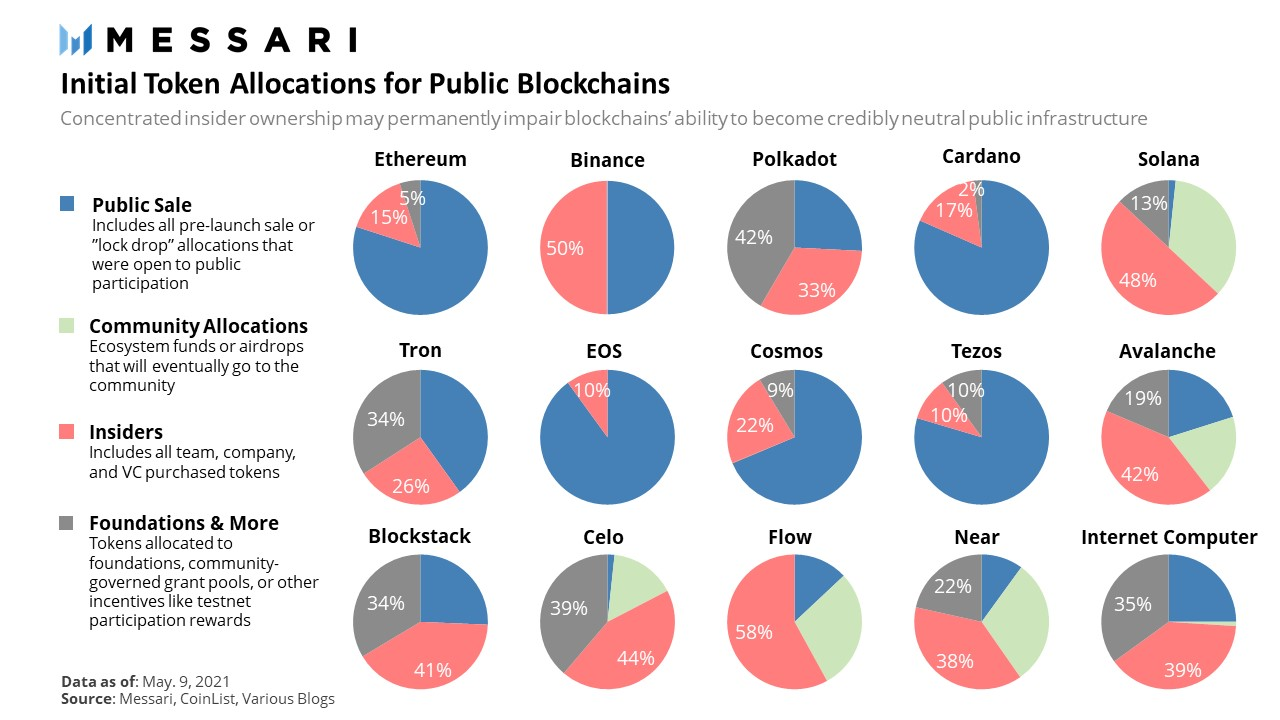
\includegraphics[width=\linewidth]{messariICO}
  \caption{Allocations given at the beginning of public blockchain, by Messari.}
  \label{fig:messariICO}
\end{figure}
\subsection{Solana}
\lipsum[50]
\subsection{AVAX}
\lipsum[50]
\subsection{Luna}
\lipsum[50]
\subsection{Crosschains}
RUNE?
\lipsum[50]
\subsection{Decentralised data}
Something about Filecoin? ARWeave? IPFS etc
\lipsum[50]


\chapter{Money in the real world}
It is necessary here to briefly examine what money actually is. In the previous section Bitcoin can be viewed in a couple of different lights. As a self custody digital bearer asset it can be viewed as `property', like gold, i.e. not a liability on someone else's asset sheet. Indeed this has long been one of the assertions of the community and it finds favour in law, \href{https://www.regulationasia.com/shanghai-court-says-bitcoin-is-protected-by-law-as-virtual-property/}{possible most ironically in China} which of course banned mining. `Money' though is a far more \href{https://www.bankofengland.co.uk/knowledgebank/what-is-money}{slippery concept} to grasp. It seems very likely that Bitcoin is evolving as a money, and it's important to define that, but there are many other kinds of money within the online world which can potentially transfer value within virtual social spaces.
\section{Defining money}
It is \href{https://www.lynalden.com/what-is-money/}{hard to find} a universally accepted definition of what money is. The best approach is to look at the properties of a thing which is asserted to be a money. In his book `A history of money', Glyn Davies identifies ``cognisability, utility,  portability, divisibility, indestructibility, stability of value, and homogeneity'' \cite{davies2010history}.\par
Stroukal examines Bitcoins' likely value as a money from an Austrian economics perspective and identifies ``portability, storability, divisibility, recognizability, homogeneity and scarcity'' \cite{stroukal2018can}.\par
A helpfully brief and useful \href{http://money.visualcapitalist.com/infographic-the-properties-of-money/}{web page by Desjardins from 2015} describes some properties and explains them in layman's terms below:
\begin{itemize}
\item Divisible: Can be divided into smaller units of value.
\item Fungible: One unit is viewed as interchangeable with another.
\item Portable: Individuals can carry money with them and transfer it to others.
\item Durable: An item must be able to withstand being used repeatedly.
\item Acceptable: Everyone must be able to use the money for transactions.
\item Uniform: All versions of the same denomination must have the same purchasing power.
\item Limited in Supply: The supply of money in circulation ensures values remain relatively constant.
\end{itemize}
\subsection{Global categories of capital}
The legacy moniker ``third world'' came from a division of the world along economic lines \cite{tomlinson2003third}. At the time this was the petrodollar / neo-institutional hegemony \cite{caballero2008financial, spiro2019hidden}, vs the economic superpower of the soviet block, and then `the rest'; unaligned economic powers.\par
This old framework has fallen away with the associated terminology, but it's useful to look at what money `is' from a global viewpoint, because all money is effectively trust in the liability held by some defined counter party.\par
Right now the dollar system is still predominant, but it seems likely that there are new axes forming, especially around the \href{https://www.wsj.com/articles/saudi-arabia-considers-accepting-yuan-instead-of-dollars-for-chinese-oil-sales-11647351541}{Chinese Yuan}. It's clear that central banks have been aware of this potential transition away from a global dollar / energy system. Policy makers have been looking back to the great economist John Maynard Keynes' ideas for a neutral basket of assets as a global synthetic hedgemonic currency \cite{carney2019growing, piffaretti2009reshaping} which would almost certainly consist partly of gold \cite{stoeferle2018gold}.\par
Use of the dollar system has recently been shown more and more to be contingent on adherence to US defined political principles. This is evidenced most starkly by the seizure of Russian central bank \href{https://twitter.com/RussianEmbassy/status/1504530573527760909}{foreign reserves}, a new and untried projection of monetary power.\par  
The Chinese Yuan/Renminbi is potentially stepping in where the petrodollar is now waning \cite{mathews2018china}. The effects of this expansion of economic influence by China, through a potential petro-Yuan, and the belt and road initiative \cite{huang2016understanding}, are not yet felt, but the lines are fairly clearly defined. The Euro system is potentially more stable, and less `weaponised' but comes with it's own restrictions for use, especially through the International Monetary Fund (IMF). It is notable for instance that the IMF have included a clause in their negotiations with Argentina to `discourage' the use of crypto based money, leading to a complete ban on banks offering the products only days after they began. This is likely a response to the adoption of Bitcoin by El Salvador, something with which the IMF is very uncomfortable. They are also wary of the ability of nation states to \href{https://www.imf.org/en/Publications/GFSR/Issues/2022/04/19/global-financial-stability-report-april-2022}{monetise their energy reserves} without the need for export markets.\par
The new `third world' who are excluded from the Dollar and/or Yuan poles of the global economy might drift toward the `basket of assets' discussed by Keynes and Carney above. As mentioned this will certainly have a component of gold, and likely other commodity assets such as rare metals. For our purposes here it's also possible that there would be a small `hedge' allocation of Bitcoin or \href{https://www.independent.co.uk/tech/bitcoin-el-salvador-crypto-btc-b2079881.html}{even a global axis} of `unaligned' nations using the asset \cite{hendrickson2021value}. This is evidenced in the early nation state adoption seen and described to date, and the game theory incentive explained by Fidelity in the introduction. It's too early to tell if this `unaligned money' could constitute a global economic pole, but it's interesting that some commentators are now even discussing this, and that \href{https://docs.google.com/document/d/1Ynl5bbdTqev-wbTAWQoeWdh1cJVf3ortuSjre9K9wGQ/edit}{carbon neutrality research} is being undertaken specifically for this application.

\section{International money transfer networks}
Transferring money from one financial jurisdiction to another is itself a global marketplace which has accreted over the entire course of human history. It's far less useful here to discuss the mythos of salt and seashells as a mechanisms of international remittance and taxation \cite{gainsford2017salt, goldberg2005famous}. Suffice it to say that there are dozens, if not hundreds, of cross border payment companies who make their business from taking a percentage cut of an international money transfer. There are also hundreds if not thousands of banks who offer this service as part of their core business portfolio. This section looks at some of the major players, and their mechanism, to contextualise the more recent shifts brought about by technology.
\subsection{Swift, ISO 20022, and correspondence banking}
Society for Worldwide Interbank Financial Communiactions (SWIFT) was initially formed in 1973 between 239 banks across 15 countries. They needed a way to improve handling of cross border payments. It is now the global \href{https://www.swift.com/standards}{standard} for financial message exchange in over 200 countries, and has recently found itself under a fresh spotlight, during the invasion of Ukraine. The system handles around 40 million short, secure, code transmissions a day, which represent crucial data about a transaction and the parties involved. It is used by both banks and major financial institutions to speed up settlement between themselves, on behalf of the clients and customers. It replaced the Telex (wire transfer) system. The new proposed and incoming standard to replace SWIFT is \href{https://www.swift.com/standards/iso-20022}{ISO20022} which is a complex and data rich arrangement. To be clear the SWIFT consortium are promoting this new standard to their 11,000 plus global user base, and there is significant investment and hype from major financial players, but it seems unclear what the actual take-up will or even should be. A group of `crytocurrencies' are heavily involved in the ISO20022 standard, and there's been experimentation with private permissioned distributed ledger technologies. It's actually somewhat unclear what value they bring, and possible that the relationship of these public ledgers to international bank to bank messaging is a marketing distraction. Note that SWIFT, ISO20022, and the associated tokens within crypto are all themselves products which have a business model. They are all intermediaries which will demand a mediating fee somewhere. All of this proposed functionality could be replaced by central bank digital currencies, which will be discussed later in the section.
\subsection{VISA etc}
VISA have announced a ``\href{https://investor.visa.com/news/news-details/2021/Visa-Introduces-Crypto-Advisory-Services-to-Help-Partners-Navigate-a-New-Era-of-Money-Movement/default.aspx}{crypto business to business support unit}''. 
\subsection{Money transfer operators}

\href{https://www.toptal.com/finance/market-research-analysts/international-money-transfer}{International Money Transfer Operators analysis}

western union etc, moneygram, transferwise,
\subsection{Digital disruptive fintech}
It seems that the neobank providers of digital banking apps are likely to converge with native digital asset ``wallets''. This is also the thesis advanced by the Ark intestments Big Ideas paper.\par
CNN have a \href{https://money.cnn.com/infographic/technology/mobile-payment-comparison/index.html}{useful primer} of the most prevalent mobile digital payment methods. This can be seen in Figure \ref{fig:CNNmobile}.
\begin{figure}
  \centering
    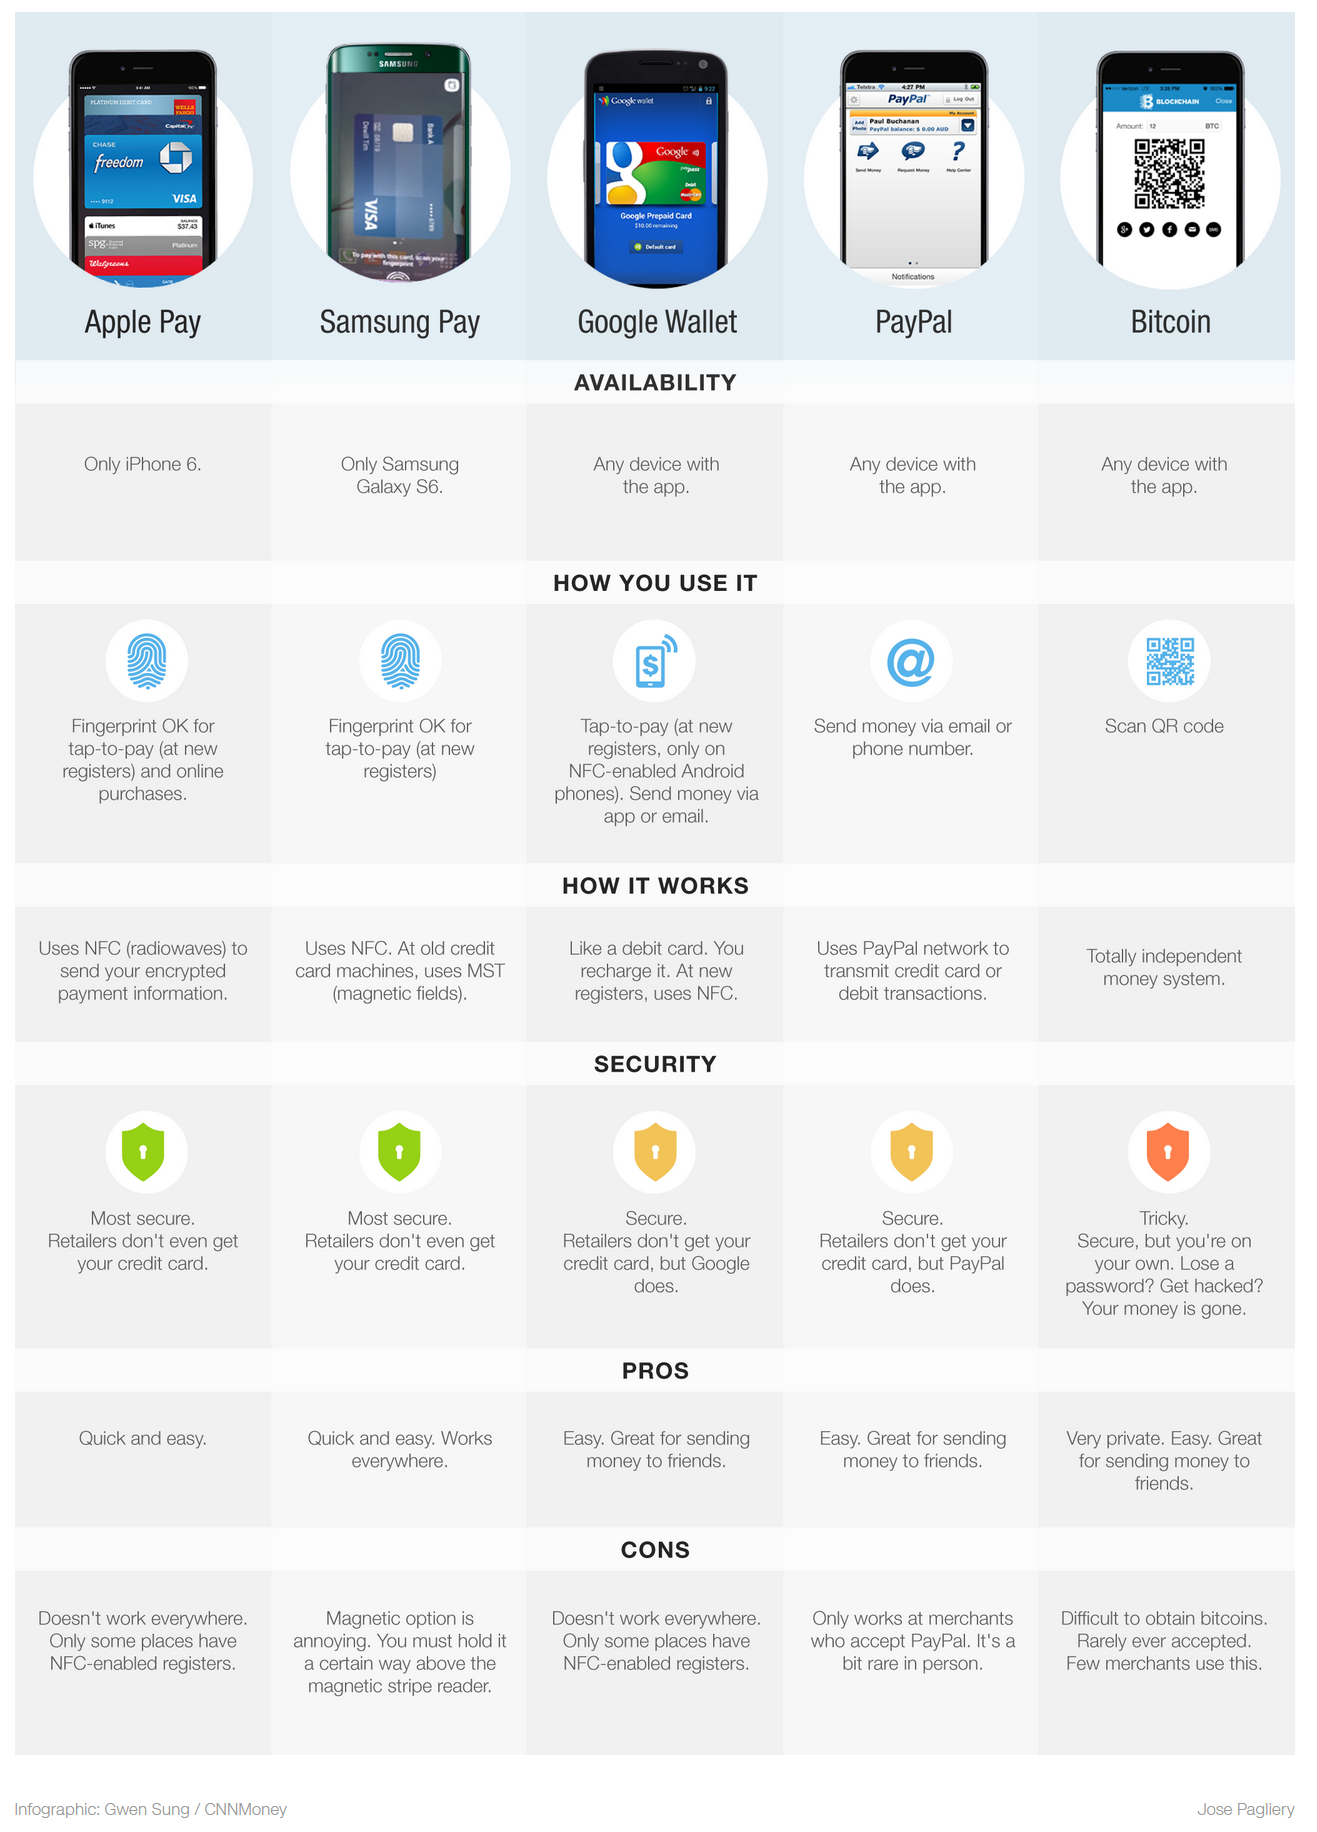
\includegraphics[width=\linewidth]{CNNmobile}
  \caption{Comparison of mobile based payment systems}
  \label{fig:CNNmobile}
\end{figure}
This comparison makes it pretty clear that Bitcoin is not ready as a personal mobile payment system. That's not to say that there isn't a place for the underlying technology in global payment processing. 
The most interesting example of this is Strike, a product in the international fintech arena. It is a `global' money transmitter which uses bank connections in local currencies, but a private version of the Lightning network with settlement on the Bitcoin main chain. In practice users connect the app to their bank and can send money to the bank connected Strike app of another user instantly, and without a fee. This is a far better product than those previously available. In principle it's open API allows many more applications to be integrated into the Strike back end. Twitter already uses this for international tipping (and remittance). It seems that this is a perfect contender for supporting transactions in open metaverse applications, and that may be true, but Strike is currently only available in three countries (USA, El Salvador, Argentina).\par
Paypal, xoom, Strike, servicing smaller payments, cashapp, venmo, revulot, 
\subsection{Stablecoins}
Stablecoins are `crypto like' instruments which are `pegged' at a 1:1 ratio with nationally issued Fiat currencies. In fact they usually correspond to units of privately issued  debt underwritten by a variety of different assets. This is (depending on the issuing company's model) a \href{https://www.americanbanker.com/opinion/ststablecoins-are-backed-by-reserves-give-us-a-break}{far more risky} unit of money than the nominal currency that they represent, but they offer significant utility. They allow the user to self custody the cryptographic bearer instrument representing the money themselves, as with blockchain. This may afford the user less friction in that they can transmit the instrument through the newer financial rails which are emerging. The caveat here is that such `units' of money can be frozen by the issuer, and they are subject to the third party risk of the issuer defaulting on the underlying instrument, instantly wiping out the value. Klages-Mundt et al. wrote a paper in 2020, which explains the details of the different mechanisms and risks.\par
The following text paraphrases Spencer noon of on-chain analytics company ``OurNetwork'', who provides an \href{https://twitter.com/spencernoon/status/1524752048121466883}{useful summary} of the paper.
\textit{There are two major classes of stablecoins:
\begin{itemize}
\item Custodial: entrusted by off-chain collateral assets like fiat dollars that sit in a bank. Requires trust in third party.
\item Non-custodial (aka decentralized): fully on-chain and backed by smart contracts \& economics. No trusted parties.
\end{itemize}
In custodial stablecoins, custodians hold a combination of assets (currencies, bonds, commodities, etc.) off-chain, allowing issuers (possibly the same entity) to offer digital tokens of an reserve asset. The top 2 custodial stablecoins today are USDT and USDC.
There are 3 types of custodial stablecoins.
\begin{itemize}
\item Reserve Fund: 100% reserve ratio. Each stablecoin is backed by a unit of the reserve asset held by the custodian. 
\item Fractional Reserve Fund: The stablecoin is backed by a mix of both reserve assets and other capital assets.
\item Central Bank Digital Currency (CBDC): A digital form of central bank money that is widely available to the general public. CBDCs are in their nascency as today only 9 countries/territories have launched them, many of them small.
\end{itemize}
Custodial stablecoins have three major risks:
\begin{itemize}
\item Counterparty Risk (fraud, theft, govt seizure, etc.)
\item Censorship Risk (operations blocked by regulators, etc.)
\item Economic Risk (off-chain assets go down in value)
\end{itemize}
Each can result in the stablecoin value going to zero.}\par
It's worth taking a look at these tokens individually, to get a feel for the trade-offs, and figure out how they might be useful for us in our proposed metaverse applications. It's important to know that these tokenised dollars and/or other currencies are issued on top of the public blockchains we have been detailing throughout. Which tokens are on what blockchains is constantly evolving, so it's not really worth enumerating specifics. In a metaverse application it would be necessary to manage both the underlying public blockchain and the stablecoin issued on top of it, making the interaction with the global financial system perversely more not less complex. In the following list of a few of the major coins, the first hyperlink is the whitepaper if it's available.
\begin{itemize}
\item \href{https://tether.to/en/whitepaper/}{Tether} is the largest of the stablecoins, with some \$80B in circulation. This has been a meteoric rise, attracting the ire and scrutiny of \href{https://www.cftc.gov/PressRoom/PressReleases/8450-21}{regulators} and \href{https://www.bloomberg.com/news/features/2021-10-07/crypto-mystery-where-s-the-69-billion-backing-the-stablecoin-tether}{investigators}. There is considerable doubt that Tether has sufficient assets backing their synthetic dollars, but the market seems not to mind. It's an important technology for this metaverse conversation because of intersections with Bitcoin through the Lightning network. Tether might actually provide everything needed. It's only as safe as the trust invested in the central issuer though.
\item Binance USD is the dollar equivalent token from global crypto exchange behemoth Binance. It's released in partnership with Paxos, who have a strong record for compliance, and transparency. Paxos also offer USDP. Both these stablecoins claim to be 100\% backed by dollars, or US treasuries. They are regulated under the more restrictive New York state financial services and have a monthly \href{https://paxos.com/attestations/}{attestation report}.
\item \href{https://makerdao.com/en/whitepaper#abstract}{MakerDAO Dai} is an Ethereum based stablecoin and one of the older offerings. It's been `governed' by a DAO since 2014. `Excess collateral', above the value of the dai-dollars to be minted, is voted upon before being committed to the systems' cryptographic `vaults' as a backing for the currency. These dai can then be used across the Ethereum network. Despite the problems with DAOs, and the problems with Ethereum, DAI is well liked by its community of users and has a healthy billion dollars of issuance.
\item \href{https://trueusd.com/pdf/TUSD_WhitePaper.pdf}{TrueUSD} claims to be fully backed by US dollars, held in escrow. It runs on the Ethereum blockchain. They have attestation reports \href{https://real-time-attest.trustexplorer.io/truecurrencies}{available on demand} and claim fully insured deposits. It's not quite that simple in that a portion of the backing is `cash equivalents'.
\item \href{https://www.gemini.com/static/dollar/gemini-dollar-whitepaper.pdf}{Gemini GUSD} claim reserves are ``held and maintained at State Street Bank and Trust Company and within a money market fund managed by Goldman Sachs Asset Management, invested only in U.S. Treasury obligations.'' which seems pretty clear.
\item \href{https://assets.website-files.com/611153e7af981472d8da199c/618b02d13e938ae1f8ad1e45_Terra_White_paper.pdf}{TerraUSD} (UST) \textbf{was} a newer and more experimental stablecoin, and one of a set of currency representations within the network. It worked in concert with the LUNA token on the Cosmos blockchain in order to keep it's dollar stability. It was not backed in the same way as the other tokens, instead relying on an arbitrage mechanism using LUNA. In essence the protocol paid users to destroy LUNA and mint UST when the price was above one dollar, and vice versa. This theoretically maintained the dollar peg. There was much concern that this model of \href{https://mirror.xyz/damsondao.eth/OVeBrmrfcWm7uKLlA2Q4W1XTVkFU3cMKfNWhgf7mQuM}{`algorithmic stable coin'} is unstable \cite{clements2021built}. The developers of the Terra tried to address this concern by \href{https://etherscan.io/address/0xad41bd1cf3fd753017ef5c0da8df31a3074ea1ea}{buying enormous amounts} of Bitcoin, which they quickly had to employ to address UST drifting downward from \$1. This failed to address the `great depegging', with LUNA crashing to essentially zero, destroying some \$50B of capital. It will now likely act as a cautionary tale to other institutions considering Bitcoin as a `reserve asset'. An \href{https://github.com/GMCyberFoundry/Metaverse/blob/b06547bf290392d2ff02e5142dae7386d888a9de/Book/04_money.tex#L186}{earlier version of this book} highlighted the specific variation of the risk which quickly manifested.
\item \href{https://f.hubspotusercontent30.net/hubfs/9304636/PDF/centre-whitepaper.pdf}{USDC} is a dollar backed coin issued by a consortium of major players in the space, most notably Circle, and Coinbase. It's has a better transparency record than tether but is still not backed 1:1 by actual dollars in reserve. It may or may not be a fractional reserve asset. It's  well positioned to take advantage of regulatory changes in the USA, and seems to be quietly lobbying to be the choice of a government endorsed digital dollar, at least a significant part of a central bank digital currency initiative. It's too early to tell how this will work out, but it has \href{https://www.forbes.com/sites/ninabambysheva/2022/04/13/blackrocks-newest-investment-paves-the-way-for-digital-assets-on-wall-street/?}{substantial `legacy finance backing'}. It is the only stablecoin to increase slightly in value (depegging upward) in the wake of the UST implosion. This `flight to quality' shows the advantage of the work that CENTRE put into regulatory compliance. If our metaverse were to pick a stablecoin to work with it would be USDC. It runs on Ethereum, Algorand, Solana, Stellar, Tron, Hedera, Avalanche and Flow blockchains. 
\end{itemize}  .

\subsubsection{The evolving US position}
In most regards the legislative front line is happening in the USA. Treasury Secretary Yellen responded to the collapse of Terra/UST \href{https://www.youtube.com/watch?v=kU0xYBRfgvU}{saying that}: \textit{``A comprehensive regulatory framework for US dollar stablecoins is needed''}. She also said that the stablecoin market is too small to pose systemic risk at this time. This is clearly an evolving situation, but the incredible consumer exposure to these risky products is likely to elicit a swift and significant response, and the timing seems right for intervention. The markets suggest that USDC will be the eventual winner.\par Koning meanwhile has looked into the different \href{http://jpkoning.blogspot.com/2021/08/stablecoin-regulatory-strategies.html}{regulatory approaches} used by various stablecoins.\par
\begin{itemize}
\item The highly regulated New York state financial framework (Paxos, Gemini)
\item Piggyback off of a (Nevada) state-chartered trust [TrueUSD, HUSD]
\item Get dozens of money transmitter licenses [USDC]
\item Stay offshore [Tether]
\end{itemize}

\href{https://www.americanbanker.com/news/toomey-unveils-stablecoin-bill-granting-occ-authority-for-payments-charter}{New legislation} specific to the concept of stablecoins is now entering the system under Sen Toomey. There are many provisions in the bill, mostly pertaining to convertibility and the ever present problem of attestation of the `backing' of these products. This is good news for this section of the digital asssets space.\par
Crucially there is also more clarity on privacy. This is a huge threat from digital money systems, and the USA is likely to lead. Remember though that none of this is yet law.\par 
Valkenburg, the lead researcher of a US think tank in digital assets \href{https://twitter.com/valkenburgh/status/1511783339065237521}{says the following}: \textit{``Stablecoin TRUST Act, is a discussion draft mostly about stablecoins, but it also has important privacy protections for crypto users broadly: it puts real limits on warrantless surveillance by narrowing what info can be collected from third parties. Last summer we fought a provision in the infrastructure bill that damaged the privacy of crypto users by expanding the broker definition (who needs to report information about transactions to the IRS) \& crypto 6050I reporting (reports on business transactions over \$10,000). The winter before we fought and successfully delayed a rushed proposal from the outgoing Trump administration to mandate that exchanges collect information about persons who are not their customers, who hold crypto at addresses in wallets they control directly. the Stablecoin TRUST Act would stop these encroachments, constrain the treasury from collecting any nonpublic information unless they get a search warrant or collect only information voluntarily provided to an exchange by a customer and for a legitimate business purpose. If “voluntarily provided for a legitimate business purpose” sounds familiar to you, that’s b/c it's the constitutional standard articulated by the Court in Carpenter describing LIMITED circumstances where warrantless searches of customer data are ok.It’s the standard we’ve advocated must also limit warrantless data collection at crypto exchanges. If exchanges must collect information about non-customers, that information is, by definition, not voluntarily provided for a legitimate business purpose.''}


%Crypto dollarisaton (myanmar)
%\href{https://twitter.com/Stacks/status/1409996245096148998}{USDC on Bitcoin?}


%It's worth pointing out that Meta (Facebook at the time) had aspirations for a global stablecoin cryptocurrency called 
%\href{https://bitcoin-red.com/facebook-libra-the-inside-story-of-how-the-companys-cryptocurrency-dream-died/}{Libre}, 
  
%\href{https://www.usdfconsortium.com/}{USDF bank issued private dollar stablecoin}

%\href{https://www.bloomberg.com/news/articles/2022-01-07/paypal-is-exploring-launc,h-of-own-stablecoin-in-crypto-push}{Paypal}


%Whatsapp, Novi, USDP etc

\subsubsection{The evolving UK position}
As mentioned briefly in the introduction the UK has recently \href{https://www.gov.uk/government/news/government-sets-out-plan-to-make-uk-a-global-cryptoasset-technology-hub}{signalled an enthusiasm} for stablecoins as ``means of payment''. This is a stark reversal of their previous legislative momentum is possibly a response to the \href{https://www.coindesk.com/policy/2022/05/11/eu-commission-favors-ban-on-large-scale-stablecoins-document-shows/}{tightening of rhetoric} in Europe around such assets. This shift clearly promotes the use of stablecoins in metaverse applications up the list of choices. 
\subsubsection{Stables in metaverse applications}
It makes a \textbf{lot} of sense to consider stablecoin transfer as the money in metaverses. USDC is furthest along this possible adoption curve. Their partnership with global payment provider Stripe has \href{https://stripe.com/blog/expanding-global-payouts-with-crypto}{enabled global dollar transfer} within Twitter for users of their `Connect' platform. This leverages the Polygon chain (mentioned in the blockchain chapter). Many digital wallets can be connected from the user end, with Metamask potentially being the easiest to integrate. This has also been mentioned in the book. The downside of this for our open platform is that none of these elements are particularly open, or distributed, and the users of the platform will still need to use an exchange to get the USDC to spend. This approach makes it easier for the vendors and product providers in the metaverse applications to accept USDC, but everything else is actually harder.

\section{Central bank digital currencies}
If 2021 was the year of the stablecoin then 2022 is likely to be the year of the central bank digital currency (CBDC). CBDCs would likely not exist without the 2019 catalyst of \href{https://www.thetimes.co.uk/article/facebooks-libra-cryptocurrency-project-ends-in-failure-cxvnnc3kx}{Facebook Libre}, \href{https://www.theguardian.com/world/2021/jul/09/currency-and-control-why-china-wants-to-undermine-bitcoin}{pressure exerted on central banks} by the concept of Bitcoin, and the stablecoins which emerged from the technology.\par
It now seems plausible that the world is moving toward a plurality of national and private digital currencies. Figure \ref{fig:CBDClikely} from the Bank for International Settlement, shows the growing acceptance within central banks. This text from the \href{https://voxeu.org/article/benefits-central-bank-digital-currency}{thinktank VoxEU} highlights the pressure on not to be `left behind': \textit{``Given the rapid pace of innovations in payments technology and the proliferation of virtual currencies such as bitcoin and ethereum, it might not be prudent for central banks to be passive in their approach to CBDC. If the central bank does not produce any form of digital currency, there is a risk that it loses monetary control, with greater potential for severe economic downturns. With this in mind, central banks are moving expeditiously when they consider the adoption of CBDC.''}\par
\ref{fig:CBDClikely}.
\begin{figure}
  \centering
    \includegraphics[width=\linewidth]{CBDClikely}
  \caption{More than half of central banks \href{https://www.bis.org/publ/bppdf/bispap125.htm}{surveyed by the BIS} said they saw issuance of a CBDC as possible.}
  \label{fig:CBDClikely}
\end{figure}
CBDCs are wholly digital representations of national currencies, and as such are centralised database entries, endorsed and potentially issued by national governments. The \href{https://www.federalreserve.gov/publications/files/money-and-payments-20220120.pdf}{USA's whitepaper} shows the approach. Curiously only \href{https://www.sanddollar.bs/about}{The Bahamas} seem to have a successful implementation, but it is a rapidly evolving space, and many nations are now scrambling to \href{https://twitter.com/GobiernoMX/status/1476376240873517061}{catch up}.\par
The following text is taken from the March 2021 Biden government ``executive order'' on digital assets, and defines the current global legislative position well.\\
\textit{``Sec. 4.  Policy and Actions Related to United States Central Bank Digital Currencies.  (a)  The policy of my Administration on a United States CBDC is as follows:\\
(i) Sovereign money is at the core of a well-functioning financial system, macroeconomic stabilization policies, and economic growth.  My Administration places the highest urgency on research and development efforts into the potential design and deployment options of a United States CBDC.  These efforts should include assessments of possible benefits and risks for consumers, investors, and businesses; financial stability and systemic risk; payment systems; national security; the ability to exercise human rights; financial inclusion and equity; and the actions required to launch a United States CBDC if doing so is deemed to be in the national interest.\\
(ii)   My Administration sees merit in showcasing United States leadership and participation in international fora related to CBDCs and in multi‑country conversations and pilot projects involving CBDCs.  Any future dollar payment system should be designed in a way that is consistent with United States priorities (as outlined in section 4(a)(i) of this order) and democratic values, including privacy protections, and that ensures the global financial system has appropriate transparency, connectivity, and platform and architecture interoperability or transferability, as appropriate.\\
(iii)  A United States CBDC may have the potential to support efficient and low-cost transactions, particularly for cross‑border funds transfers and payments, and to foster greater access to the financial system, with fewer of the risks posed by private sector-administered digital assets.  A United States CBDC that is interoperable with CBDCs issued by other monetary authorities could facilitate faster and lower-cost cross-border payments and potentially boost economic growth, support the continued centrality of the United States within the international financial system, and help to protect the unique role that the dollar plays in global finance.  There are also, however, potential risks and downsides to consider.  We should prioritize timely assessments of potential benefits and risks under various designs to ensure that the United States remains a leader in the international financial system.''}\par

In traditional nation state currencies the central banks \href{https://www.bankofengland.co.uk/markets/bank-of-england-market-operations-guide}{control the amount} of currency in circulation by issuing debt to private banks, which is then loaned out to individuals \cite{wang2021central}. The debt is `destroyed' on the balance sheet to remove currency through the reverse mechanism. They also facilitate government debt \cite{filardo2012central}, and work (theoretically) outside of political control to adjust interest rates, in order to manage growth and flows of money. \par
Many things which cannot be done with traditional nation state money systems are possible with CBDCs, because they \href{https://voxeu.org/article/benefits-central-bank-digital-currency}{remove the middleman} of private banking between the end user and the policy makers. 
\begin{itemize}
\item Negative interest rates are possible, such that all of the money can lose purchasing power over time, and at a rate dictated by policy. This ``removal of the lower bound'' has been discussed by economists over the last couple of decades as interest rate mechanisms have waned in efficacy. It is not possible in the current system, and instead money must be added through \href{https://www.bankofengland.co.uk/monetary-policy/quantitative-easing}{quantitative easing}, which disproportionately benefits some though Cantillon effects \cite{cantillon1756essai, bordo1983some}.  
\item Ubiquitous basic income is possible in that money can be issued directly from government to all approved citizens, transferring spending power directly from the government to the people. This also implies efficiency savings for social support mechanisms.
\item Asset freezing and confiscation are trivial if CBDCs can replace paper cash money completely, as a bearer asset. Criminals and global `bad actors' could have their assets temporarily or permanently removed, centrally, by suspending the transferability of the digital tokens.
\item Targeted bailouts for vital institutions and industries are possible directly from central government policy makers. Currently private banks must be incentivised to make cheap loans available to sectors which require targeted assistance.
\item Financial surveillance of every user is possible. In this way a `panopticon of money' can be enacted, and spending rulesets can be applied. For instance, social support money might only be spendable on food, and child support only on goods and services to support childcare. This is a very dystopian set of ideas. Eswar Prasad says ``In authoritarian societies, central bank money in digital form could become an additional instrument of government control over citizens rather than just a convenient, safe, and stable medium of exchange.'' \cite{prasad2021future}
\item It's a virtually cost free medium of exchange, since there is no physical instrument which must be shipped, guarded, counted, assayed, and securely destroyed.
\item The counterfeiting risk is significantly reduced because of secure cryptographic underpinnings rather than paper or plastic anti counterfeiting technologies.
\item Global reach and control is instantly possible for the issuer. This is a big problem especially for a reserve currency such as the dollar. Two thirds of \$100 bills are \href{https://www.federalreserve.gov/pubs/ifdp/2012/1058/default.htm}{thought to} reside outside of the USA.
\item System level quantitative easing and credit subsidies are made far simpler and less wasteful when centrally dictated.
\item Transfer of liability and risk to the holder globally reduces the management costs for global deposits of a currency. 
\item It may be possible to automate the stability of a currency through continuous adjustment of the `peg' through algorithms or AI.
\end{itemize}

The UK has signalled that it is not interested in developing a CBDC at this time. It is viewed as a \href{https://committees.parliament.uk/publications/8443/documents/85604/default/}{solution in search of a problem}, with the Lords economic affairs committee saying:\textit{``The introduction of a UK CBDC would have far-reaching consequences for households, businesses, and the monetary system for decades to come and may pose significant risks depending on how it is designed. These risks include state surveillance of people’s spending choices, financial instability as people convert bank deposits to CBDC during periods of economic stress, an increase in central bank power without sufficient scrutiny, and the creation of a centralised point of failure that would be a target for hostile nation state or criminal actors.''}\par
Meanwhile in Europe, ECB President \href{https://www.ecb.europa.eu/press/pressconf/2022/html/ecb.is220310~1bc8c1b1ca.en.html#qa}{Christine Legarde} said: \textit{``On your question concerning CBDC, you know my views on CBDC and you know that I have pushed that project. Fabio Panetta is working hard on that together with members in the entire Eurosystem with the high-level taskforce that is working really hard on moving forward. But in a way, I am really pleased that attention is now focussed on the role that cryptos can play and the role that Central Bank Digital Currency can have when they are implemented. We have a schedule, as you know. The Governing Council decided back in October '21 to launch a two-year investigation phase, and it is at the end of that investigation phase that the decision will definitely be made to launch the CBDCs and to make it a reality. We can't go wrong with that project. I am confident that we will move ahead, but that's going to be a decision of the Governing Council. I think it's an imperative to respond to what the Europeans expect, and I think we have to be a little bit ahead of the curve if we can on that front. If we can accelerate the work, I hope we can accelerate the work. I will certainly support that and I was delighted to see that in the United States there was an executive order by President Biden to actually expect similar effort and focus and progress on CBDC, cryptos. I think that it will take all the goodwill of those who want to support sovereignty, who want to make sure that monetary policy can be transmitted properly using our currency, will endeavour.''}\par
In the USA this text from Congressman Tom Emmer shows how complex and interesting this debate is becoming.\textit{``Today, I introduced a bill prohibiting the Fed from issuing a central bank digital currency directly to individuals. Here’s why it matters: As other countries, like China, develop CBDCs that fundamentally omit the benefits and protections of cash, it is more important than ever to ensure the United States’ digital currency policy protects financial privacy, maintains the dollar’s dominance, and cultivates innovation.\\
CBDCs that fail to adhere to these three basic principles could enable an entity like the Federal Reserve to mobilize itself into a retail bank, collect personally identifiable information on users, and track their transactions indefinitely.\\
Not only does this CBDC model raise ``single point of failure'' issues, leaving Americans’ financial information vulnerable to attack, but it could be used as a surveillance tool that Americans should never be forced to tolerate from their own government.\\
Requiring users to open an account at the Fed to access a United States CBDC would put the Fed on an insidious path akin to China’s digital authoritarianism.\\
Any CBDC implemented by the Fed must be open, permissionless, and private. This means that any digital dollar must be accessible to all, transact on a blockchain that is transparent to all, and maintain the privacy elements of cash.\\
In order to maintain the dollar’s status as the world’s reserve currency in a digital age, it is important that the United States lead with a posture that prioritizes innovation and does not aim to compete with the private sector.\\
Simply put, we must prioritize blockchain technology with American characteristics, rather than mimic China’s digital authoritarianism out of fear.''}\par
Most analysts now seem to think that there is little appetite to replace all of a given currency with a CBDC. It is far more likely that a blend of stablecoins, private bank issued digital currency (with a yield incentive) and some limited CBDC, alongside the new contender Bitcoin, will present a new landscape of user choice. Different models of trust, insurance, yields, acceptability, and potentially privacy, will emerge. \par
Clearly a global, stable, wholly digital bearer asset in a native currency would be the ideal integration for money in a metaverse application, but it is likely that a transition to such a technology would be complex and painful. It is certainly not ready for consideration now.
\section{Bitcoin as a money}
\subsection{Spending it}
Since this book seeks to examine transfer of value within a purely digital environment it is necessary to ask the question of whether Bitcoin is money. This short \href{https://bitcoin-zar.blogspot.com/2018/07/duality-excerpt-by-satoshi-nakomoto.html}{`story'}, purportedly written by Nakamoto, is a fabulous look at the money values of the technology, irrespective if it's provenance. In it is the following text: \textit{``Here, for once, was this idea that you could generate your own form of money. That's the primary and sole reason, is because it was related to this thing called money. It wasn't about the proficiency of the code or the novelty, it was because it had to do with money. It centered around money. That is something people cared about. After all, plenty of projects on Sourceforge at the time were just as well coded, well maintained, if not better, by teams, and even if someone else had created the blockchain before me, had it been used for something else beyond currency, it probably would not have had much of an outcome.}\par
Again, irrespective of the author here, this point seems to ring true. The memetic power of Bitcoin is in it's proximity to `money'.\par
It is beyond argument that the Bitcoin network is a rugged message passing protocol which achieves a high degree of consensus about the entries on it's distributed database.\par Ascribing monetary value to those database entries is a social consensus problem, and this itself is a contested topic. The most useful `hot take' here is that Bitcoin behaves most like \href{https://twitter.com/saylor/status/1395788419301773312}{a `property'}, while it's network behaves far more like a monetary network. \par
Jack Mallers, of Strike \href{https://www.youtube.com/watch?v=jb-45m9f76I}{presentation to the IMF} identified the following challenges which he claims are solved by the bitcoin monetary network.
\begin{itemize}
\item Speed
\item Limited transparency and dependability
\item High cost
\item Lack of interoperability
\item Limited Coverage
\item Limited accessibility
\end{itemize}
He further identifies the attributes of the ideal global money. 
\begin{itemize}
\item Uncensorable
\item Unfreezable
\item Permissionless
\item Borderless
\item Liquid
\item Digital
\end{itemize}
Mallers has recently announced USA focused partnerships which leverage his Strike product to enable spending Bitcoin, through Lightning, as Dollars in much of the \href{https://www.ncr.com/point-of-sale-pos-systems}{point of sale} infrastructure in the USA. This is a huge advance as it immediately enables the vendors both online and at physical locations to either save 3\% costs for card processors, or else pass this on as a discount. Crucially for `Bitcoin as a money' it also allows the vendors to receive the payment \textbf{as} Bitcoin, not Dollars. A possible further and highly significant feature is that it might now be possible to divest of Bitcoin in the USA, buying goods, without a capital gains tax implication. Mallers claims to have legislative backing for this product, but the devil will likely be in the detail. The likely mechanism for this product is that the EPOS partner sends a Lighting request to Strike, which liquidates some of their Bitcoin holding to a dollar denominated stablecoin, but in a tax free jurisdiction such as El Salvador. This stablecoin will then be sent to the EPOS handing partner such as NCR. Stablecoin to Dollar transactions in the USA are much murkier and likely don't cost anything for these companies. This agent will then authorise the Dollar denominated sale to the American digital till. Crucially nobody has a US capital gains tax exposure in this chain, and all of the settlements were near free, and instantaneous, with `cash finality' for everyone except the EPOS company. They are likely actually exposed to a small risk here because uptake will be very low level. The novelty opportunity will likely cover any potential exposure to stablecoin collapse. This is a radical upgrade on the normal flow of divesting Bitcoin for American users. \par
Using this open product to spend Bitcoin as Bitcoin to vendors might be available through Shopify globally. Again, it's too new to be sure.\par
Of these recent developments in Lightning \href{https://twitter.com/LynAldenContact/status/1512188883101966351}{Lyn Alden says}: \textit{Some people naturally dismiss [strike] because they don't want to spend their BTC; they want to save it. However, the more places that accepted BTC at point of sale (on-chain or Lightning or otherwise), the more permissionless the whole network is. This is because, if all you can do with BTC is convert it back into fiat on a major exchange, then it's easy to isolate it, effectively blacklist addresses, etc. But if you can directly spend it on goods and services across companies and jurisdictions, it's harder to isolate. There are now plenty of vendors that make this easy for merchants to implement, and the merchant can still receive dollars if they want (rather than BTC), or can decide their \% split. Since it's an open network, anyone can build on it, globally. And then when you add fiat-to-BTC-to-fiat payments over Lightning, it gets even more interesting because it doesn't necessarily need to be a taxable event. Lightning wallets with a BTC balance and a USD/stablecoin balance. Lower fees than Visa and others.}\par
More interestingly for metaverse applications Mallers has opened this section of the company to interact with the public Lightning network, allowing people with a self hosted wallet or node to pay directly for goods across America, settling immediately in Dollars, using their Bitcoin, at zero cost. \textbf{This opens the possibility to buy from US based (Dollar denominated) metaverse stores, using the capabilities of the stack assembled at the end of the book}. The implications globally are unclear at this time.\par
\subsection{Saving with it} 
The Bitcoin community believes that \href{https://svetski.medium.com/why-bitcoin-not-shitcoin-6cc826f4fa52}{Bitcoin is the ultimate money}, a \href{https://www.coindesk.com/business/2022/01/07/jpmorgan-sees-more-crypto-adoption-in-2022-debates-bitcoins-status-as-store-of-value/}{`store of value'}, chance to \href{https://www.forbes.com/sites/leeorshimron/2020/06/30/bitcoin-is-the-separation-of-money-and-state/?sh=49294a8356db}{separate money from state}, increase \href{https://www.washingtonpost.com/national/locked-out-of-traditional-financial-industry-more-people-of-color-are-turning-to-cryptocurrency/2021/12/01/a21df3fa-37fe-11ec-9bc4-86107e7b0ab1_story.html}{equality of opportunity} and \href{https://iai.tv/articles/the-rich-get-richer-the-poor-get-bitcoin-auid-1766}{ubiquity of access}, while others view it as \href{https://www.cnbc.com/2021/06/22/a-third-of-investors-think-bitcoin-is-rat-poison-jpmorgan-survey-says.html}{`rat poison'}, or a \href{https://jacobinmag.com/2022/01/cryptocurrency-scam-blockchain-bitcoin-economy-decentralization}{fraudulent Ponzi scheme}. A notable exclusion from the negative rhetoric is Fidelity, the global investment manager, who have always been positive and have \href{https://www.fidelitydigitalassets.com/articles/bitcoin-first?sf253214177=1}{recently said}: 
\textit{``Bitcoin is best understood as a monetary good, and one of the primary investment theses for bitcoin is as the store of value asset in an increasingly digital world.''}\par
The following paraphrases Eric Yakes, author of \href{https://yakes.io/book/}{`The 7th Property'}. Again, this is an Austrian economics perspective, and like much economic theory the underlying premise \href{https://medium.datadriveninvestor.com/do-you-understand-the-austrian-vs-keynesian-economic-debate-2f4b152c6a6b}{is contested}\cite{maurel2012keynesian}: \textit{``Paper became money because it was superior to gold in terms of divisibility and portability BUT it lacked scarcity. People reasoned that we could benefit from the greater divisibility/portability of paper money as long as it was redeemable in a form of money that was scarce. This is when money needed to be ``backed'' by something. \\
Since we changed money to paper money that wasn't scarce, it needed to be backed by something that was. Since the repeal of the gold standard, politicians have retarded the meaning of the word because our money is no longer backed by something scarce.\\
So, what is bitcoin backed by? Nothing.\\
Sound money, like gold, isn’t ``backed''.
Only money that lacks inherent monetary properties must be backed by another money that maintains those properties. The idea that our base layer money needs to be backed by something is thinking from the era of paper money. Bitcoin does not require backing, it has inherent monetary properties superior to any other form of money that has ever existed.''}\par
The 2022 ARK Big Ideas report again provides some useful market insight. They posit that demand for the money features of Bitcoin could drive the price of the capped supply tokens to around 1M pounds per Bitcoin as in Figure \ref{fig:BitcoinShareOfMoney}. Take this with the usual pinch of salt, as Ark have been performing notably badly lately with their predictions.
\begin{figure}
  \centering
    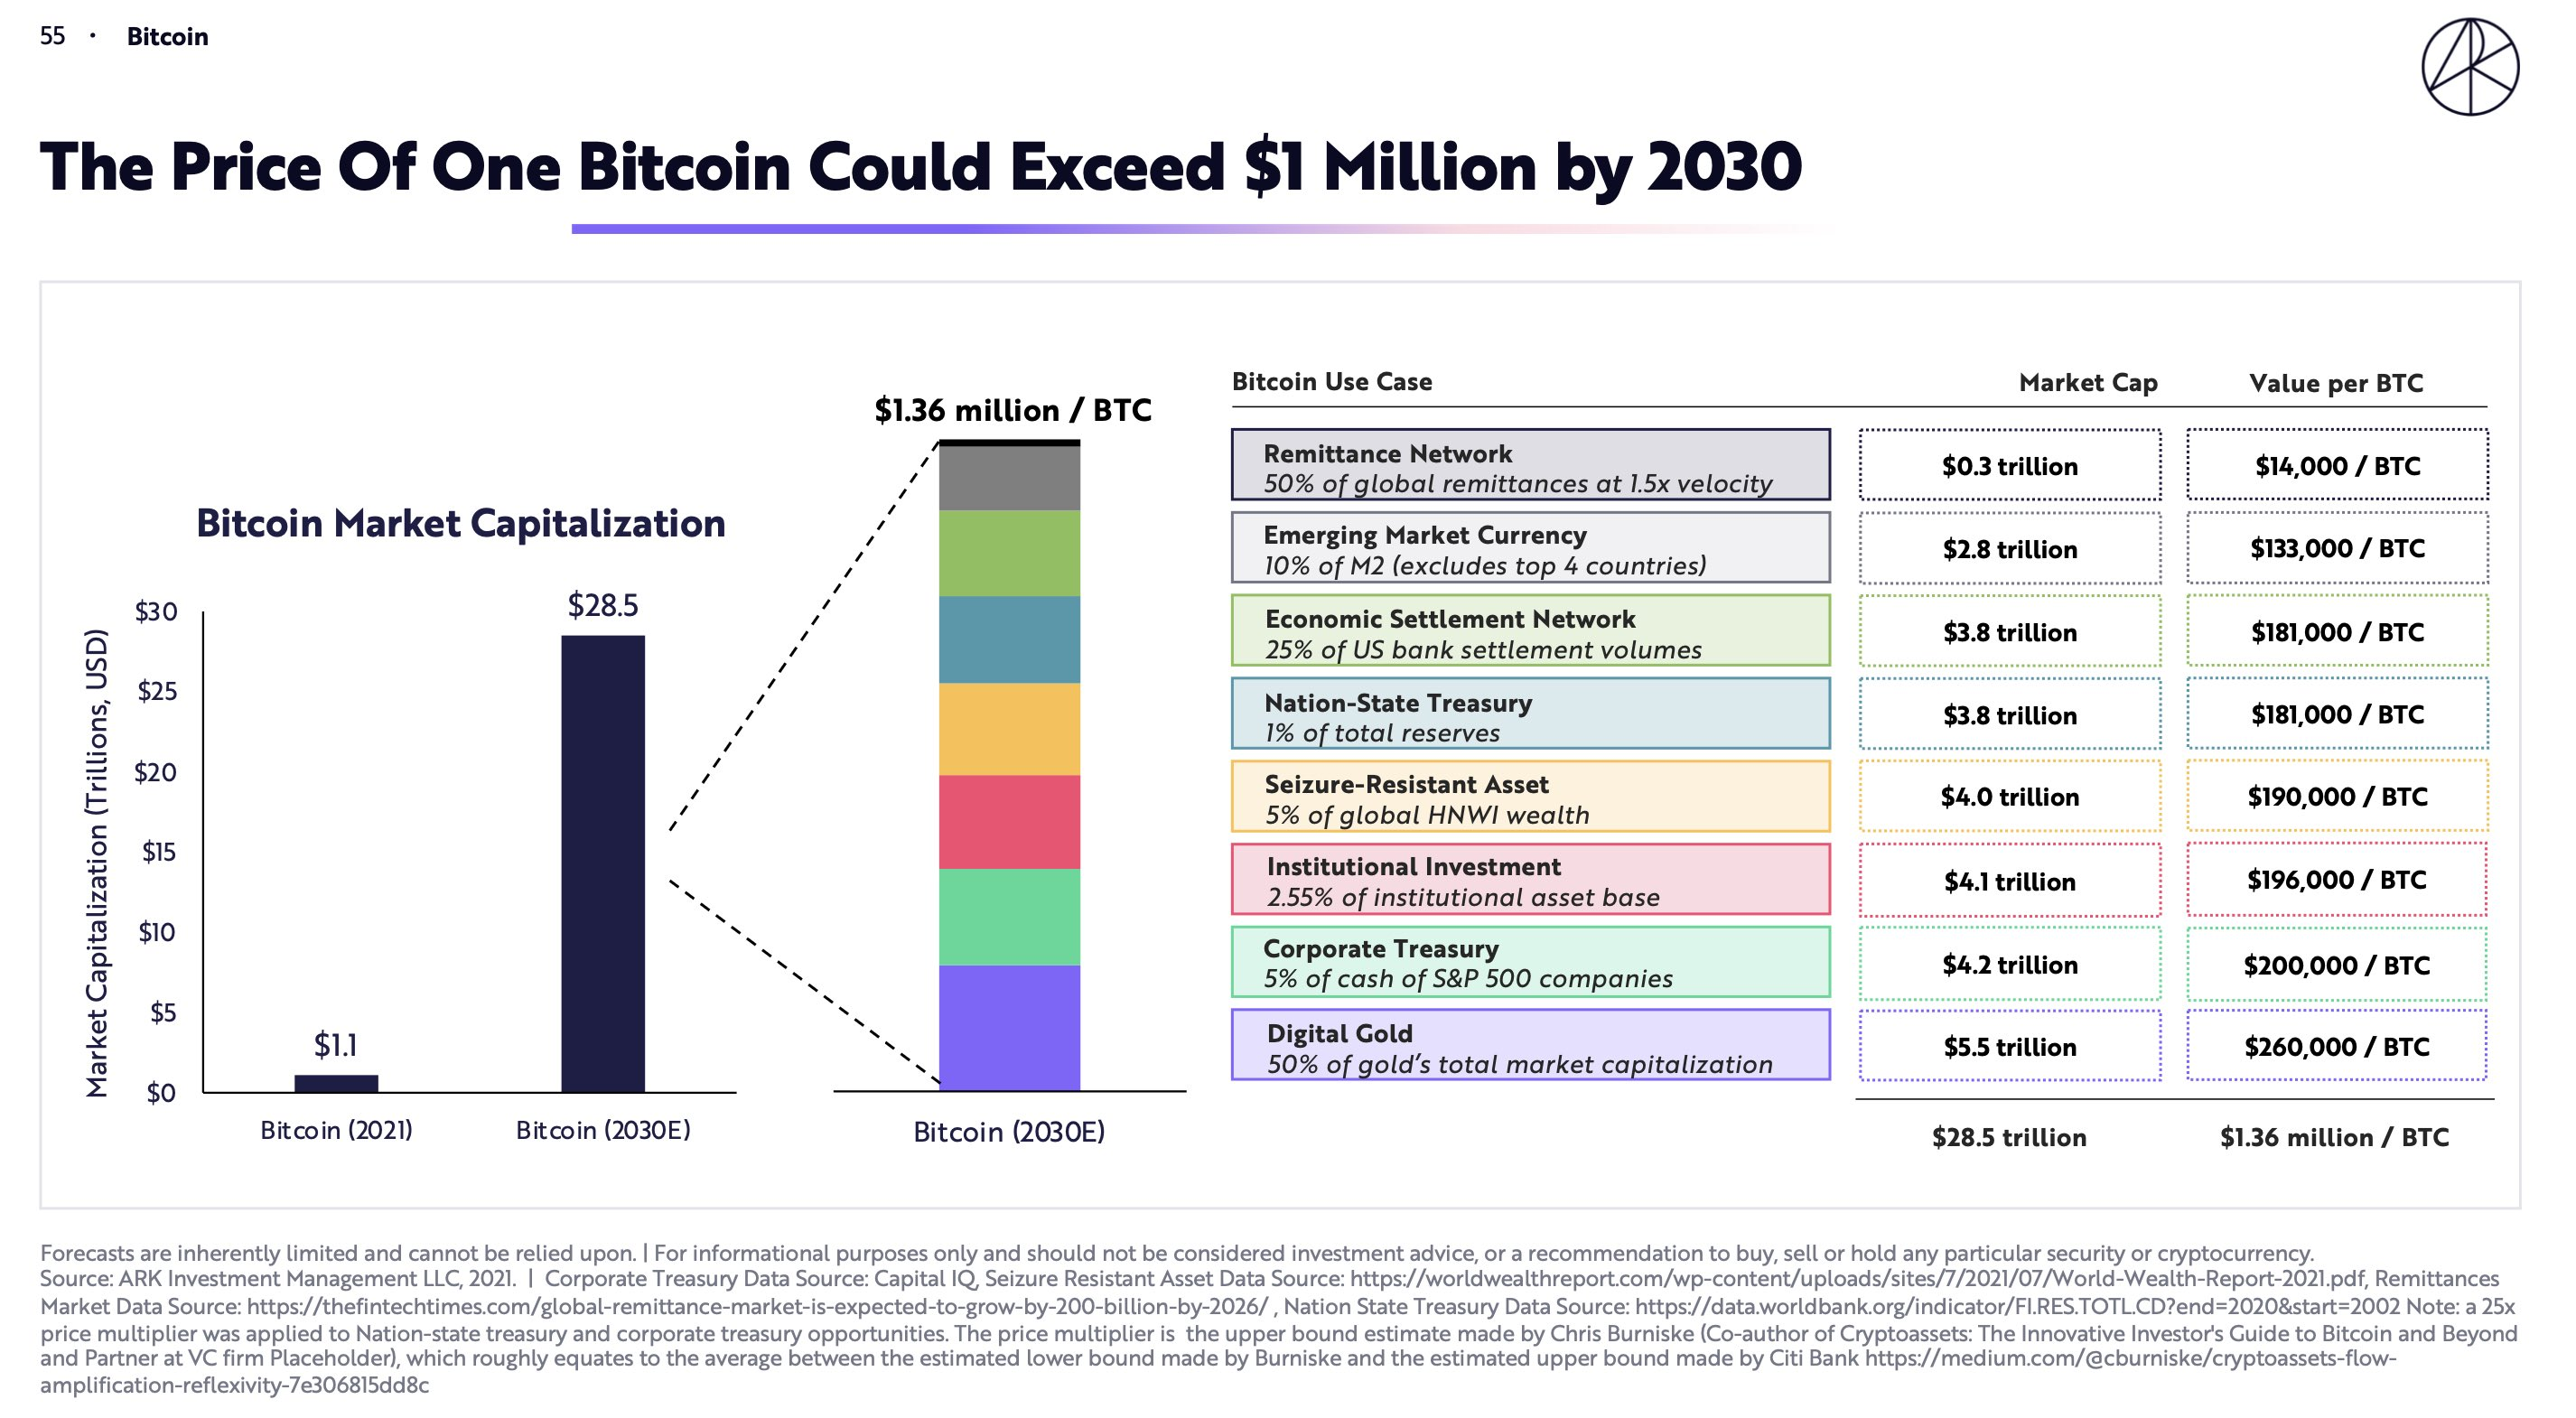
\includegraphics[width=\linewidth]{BitcoinShareOfMoney}
  \caption{Potential market exposure to Bitcoin as a money}
  \label{fig:BitcoinShareOfMoney}
\end{figure}
Perhaps more than any of these takes, it is worth considering the current public perception of the technology as a money and store of value. This \href{https://twitter.com/saquon/status/1480738426236375041}{twitter thread} from professional sportsman Saquon Barkley, to his half million followers on the platform, captures the mood. He is one of a handful of athletes now being \href{https://www.buybitcoinworldwide.com/athletes/}{paid directly} in Bitcoin.\par
\textit{``I want my career earnings to last generations. The average NFL career is 3 years and inflation is real. Saving and preserving money over time is hard, no matter who you are.
In today’s world: How do we save? This is why I believe in bitcoin. Almost all professional athletes make the majority of their career earnings in their 20s. With a lack of education, inaccessible tools, and inflation, a sad yet common reality is many enter bankruptcy later on. We can do better. We need to improve financial literacy. Bitcoin is a proven, safe, global, and open system that allows anyone to save money. It is the most accessible asset we’ve ever seen.''}\par
This ubiquity of access is what probably most distinguishes Bitcoin. Previously it could be argued that only the most wealthy could access the `means' to store their labour without loss of value over time (through inflation). To be clear, inflation is an important part of the money system, somewhat within the control of the central banks, and approximate to taxation. It applies equally to all holders of the money supply. Asserting that money should be replaced by a `hard asset' such as Bitcoin, in the place of the more controllable utility of money, is likely both a fantasy, and wrong minded. This conflation of money and property is a confusion caused by Bitcoin's proximity to money, and it's `money like' network, and is extremely commonplace.\par
These narrative takes are all rooted in the popular idea that Bitcoin is a `hedge against inflation'. The Bitcoin community seems somewhat confused about the nature of money, which is predictable because we can see in these sections that money is pretty confusing. Money is the fluid thin `working' layer on top of historical human production, which provides transaction convenience, and tools for credit. Value is effectively swapped in and out of this layer through the actions of central banks, controlling inflation into acceptable margins. Simplistically this is done through manipulation of interest rates (the easiness of credit), quantitative easing (buying of assets) and quantitative tightening (selling of assets). It is primarily \textit{not} a long term store of value, as Austrian economists perhaps believe it should be. This function is left to assets.\par 
Fundamentally, Bitcoin isn't money (in the traditional sense) because it's not an IOU, which money certainly is. It's a bearer instrument, novel asset class, with money like properties, as identified above. As said again and again it functions most like a `property' which can be invested in by anyone, with all the attendant risks of that property class to the holder. Lyn Alden says it sits \href{https://www.lynalden.com/what-is-money/}{somewhere between} a saving tool, and an investment, acting as ``programmable commodity money''.\par 
\href{https://andrewmbailey.com/}{Andrew M. Bailey} says \textit{``in an ideal world where governments honour the rights of citizens, they don't spy, they don't prohibit transactions, they manage a sound money supply, and they make sound decisions, the value of bitcoin is very low; we're just not in an ideal world''}\par
Another potentially important differentiating affordance is censorship resistance. There's really nothing else like it for that one feature. With that said Bitcoin is only a viable `money like thing' when viewed in the layers described in this book, \href{https://giacomozucco.com/layers-before-bitcoin}{and elsewhere}\cite{Bhatia2021}. The base chain layer is an apex secure store of value. Whatever layer 2 ultimately emerges is the transactional layer which could replace day to day cash money, while the hypothetical layer 3 might be useful for complex financial mechanisms and contracts operating automatically, and also provides the opportunity for using the security model of the chain to support other digital assets, including government currencies through stablecoins. All these things have a natural home in borderless social spaces.
\section{Risks (money, not technical)}
Special thanks to economist Tim Millar for help with this section.
\subsection{Risks to Bitcoin the money}
It can be seen that following the invasion of Ukraine by Russia, that sanctions of various kinds were applied to the Russian economy. One of these was the previously dicussed Swift international settlement network. Another whole catagory was the removal of support by private businesses domiciled outside of Russia and Ukraine, and pertinent here is that VISA, Mastercard, Paypal, and Western Union all removed support for their product rails. This means that while some cards and services still work, and will likely work again through Chinese proxies in the coming months, considerable disruption will be felt by Russian companies and individuals. This is not to say that this disruption is necessarily wrong, but it is clear now that all of these global financial transfer products and services are contingent on political factors. The same might be true of CBDC products if they gain traction globally. There is certainly no reason why all money within a physically delineated border could not be blocked or cancelled. This is not as true for Bitcoin at this time. \par 
However, with enough political will it is technically plausible to incentivise miners with additional payments to exclude transactions from geolocated wallets. This would be mitigated by Tor, and in a global anonymous network it is very likely that a miner could be found at a higher price for inclusion in the next block. \par
Bitcoin is still young and illiquid enough to be highly manipulable. Imagine for instance if a major organisation or nation state wished to accumulate a significant amount of the asset, but would prefer a lower price. %To pick a mechanism at random, they could force a de-pegging of UST in the Terra/Luna ecosystem, forcing the algorithmic selling of Do Kwon's multi-billion dollar Bitcoin reserve contingency. This would immediately crash the price. 
Nobody knows just how vulnerable to selling cascades Bitcoin might be against a really serious challenge by an empowered actor, but it's already high volatility is suggestive of risk. It's also vulnerable to rehypothecation (paper bitcoin managed by centralised entities running a fractional reserve). It seems that Figure \ref{fig:talebturkey} by  Nassim Taleb is a cautionary tale \cite{taleb2012antifragile}.
\begin{figure}
  \centering
    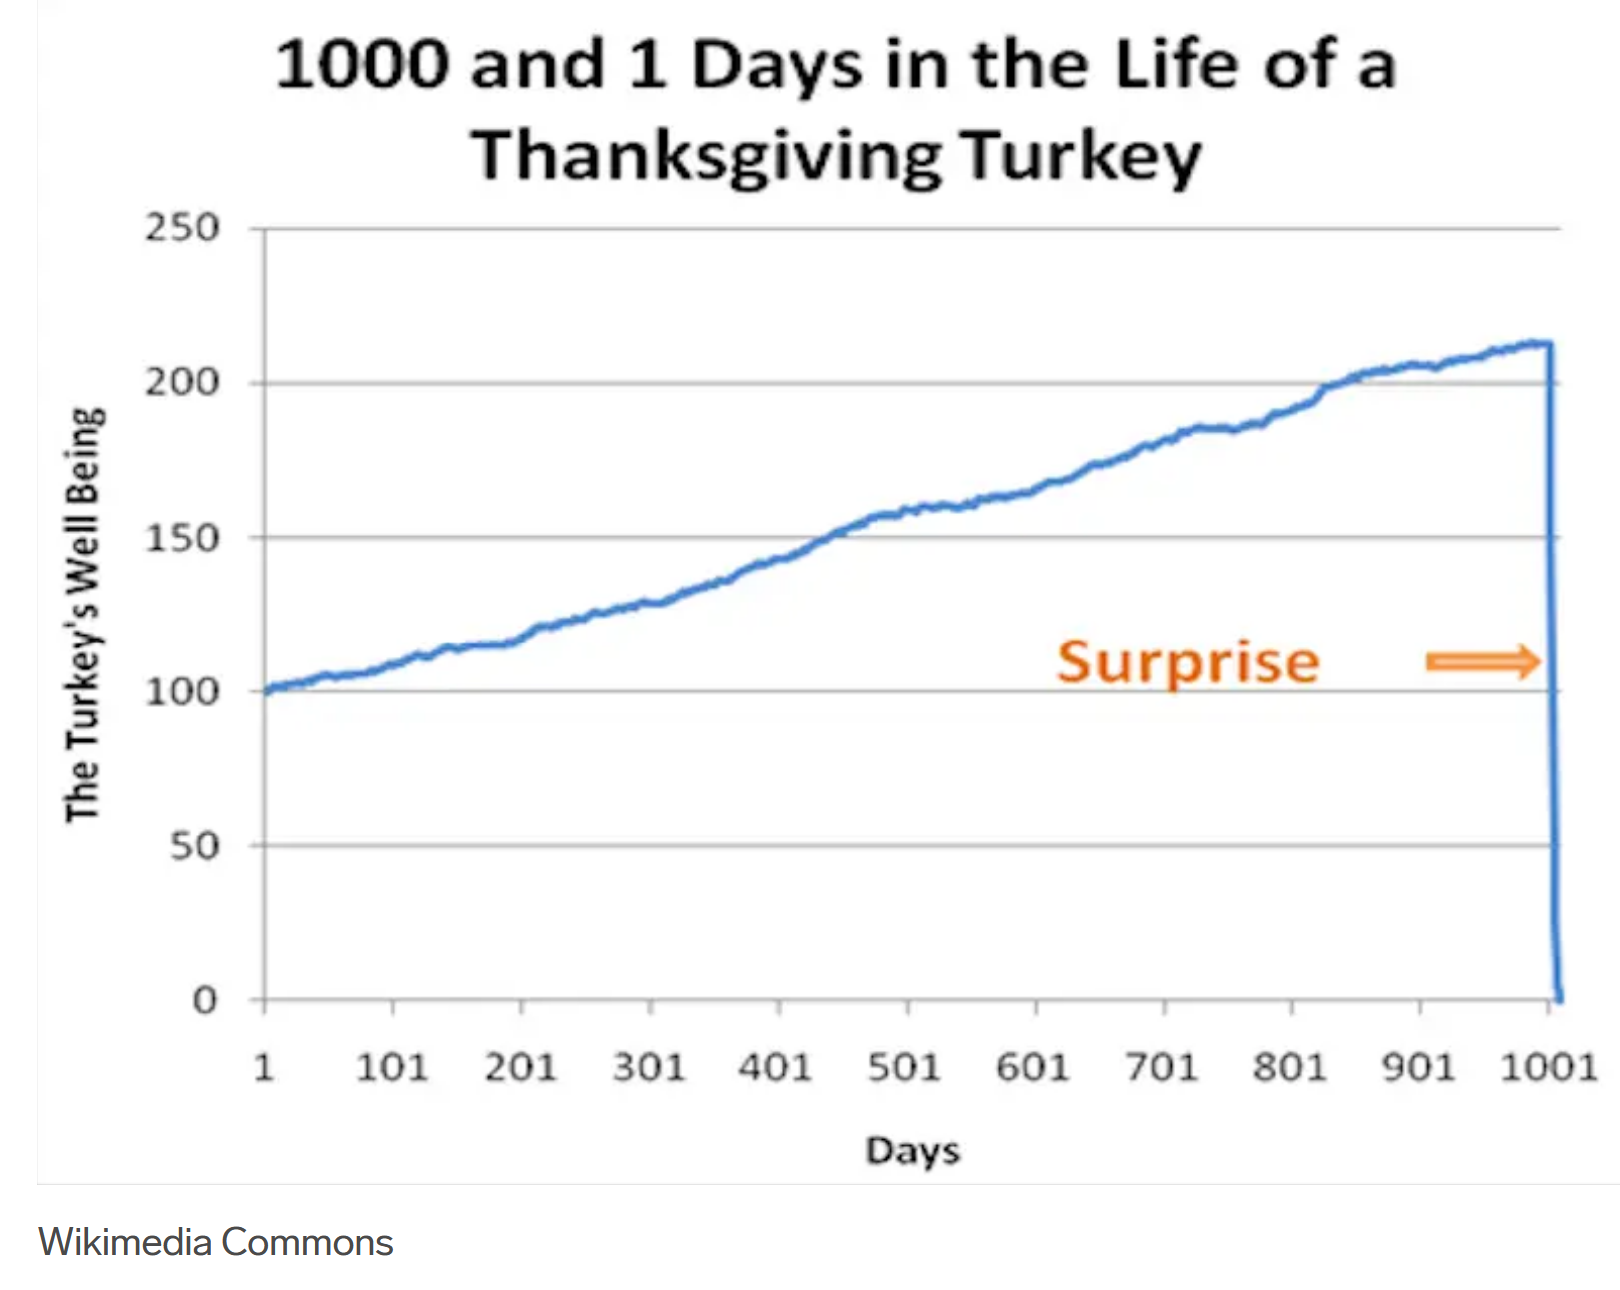
\includegraphics[width=0.7\linewidth]{talebturkey}
  \caption{Nassim Taleb's Turkey Problem}
  \label{fig:talebturkey}
\end{figure}

Scalability is always going to be a problem for Bitcoin, for all the reasons discussed in the blockchain chapter.\par 
Finally, a lack of fungibility, and privacy by default in Bitcoin, trends towards blacklists and over time this could seriously compromise the use of the asset. The next section is the risks that Bitcoin poses to external money systems, but it's worth pointing out that a risk to wider society is clearly \textit{also} a risk to Bitcoin itself.
\subsection{Bitcoin externalities}
\subsubsection{Inherent volatility}
One of the better public analysts of the asset, \href{https://twitter.com/davthewave/status/1072441941390974982/photo/1}{sees the price} eventually fluctuating somewhere between ~\$200k and ~\$30k.  Figure \ref{fig:davethewave}. This is not how a money is supposed to work. 

\begin{figure}
  \centering
    \includegraphics[width=\linewidth]{davethewave}
  \caption{\href{https://davethewave.substack.com/p/cycle-theory-revisited?s=r}{Cycle theory revisited blog post} [Image used with permission]}
  \label{fig:davethewave}
\end{figure}

Neither though is it the endless \href{https://stephanlivera.com/episode/147/}{``number go up''} that speculators have been promised. The aims of the project have a cognitive dissonance right at the core. The volatility trends toward:
\subsubsection{Unfair distribution}
By design the distribution of Bitcoin is likely `fair`, in that everyone has been able to access and secure the asset long term without prejudice. Figure \ref{fig:btcdistribution} from Twitter user @Geertjancap shows the distribution in 2021. Whether this is judged to be fair if the asset jumps to 10 times it's current value, minting a new class of hyper rich holders, is another matter. 
\begin{figure}
  \centering
    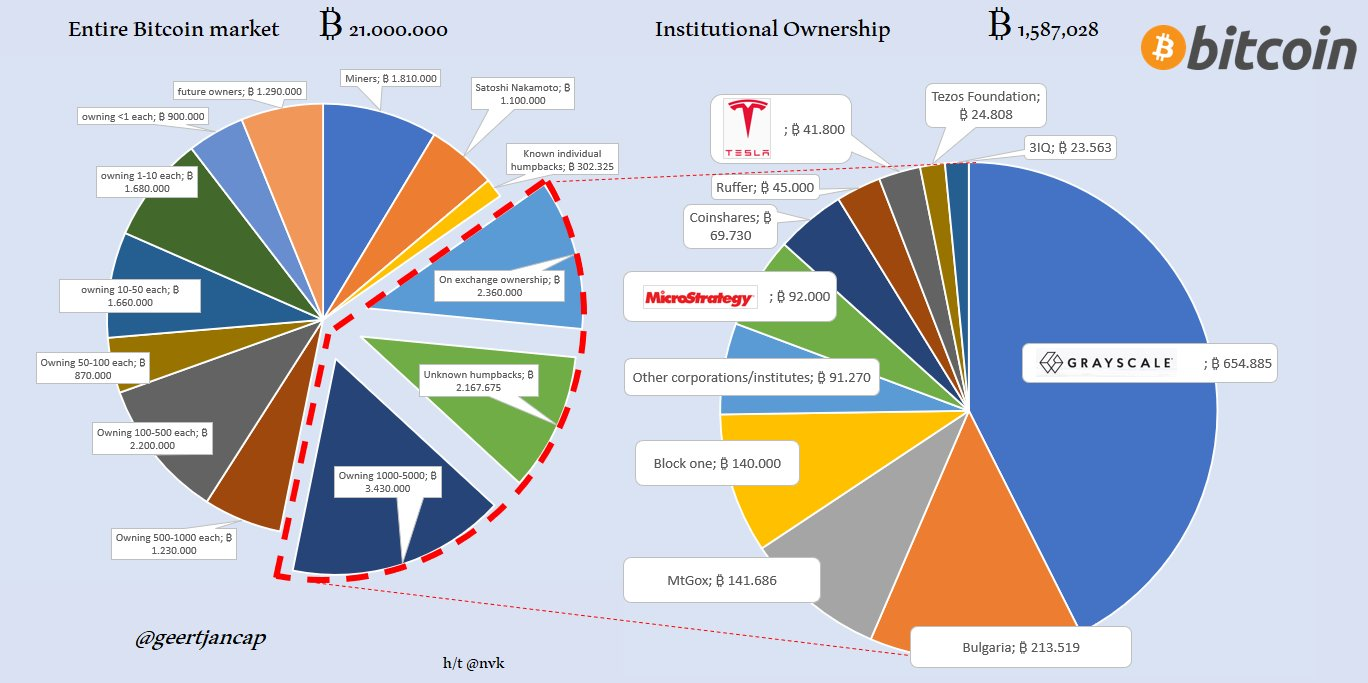
\includegraphics[width=\linewidth]{btcdistribution}
  \caption{\href{https://twitter.com/Geertjancap/status/1380972132990136322/photo/1}{Bitcoin distribution is skewed to s few early holders, but it likely \textbf{is} fair.} [Image used with permission]}
  \label{fig:btcdistribution}
\end{figure}
This pressure to emulate the early winners leads to:
\subsubsection{Endless HODL}
It's possible that there's a problem with people not wanting to sell the asset, because they are predisposed to a particular fervour promoted within the community. This can be seen in the \href{https://twitter.com/DylanLeClair_/status/1521123370233962497}{glassnode data}, where the black line in Figure \ref{fig:notselling} shows that the asset held for more than a year (illiquid) has increased over the years.
\begin{figure}
  \centering
    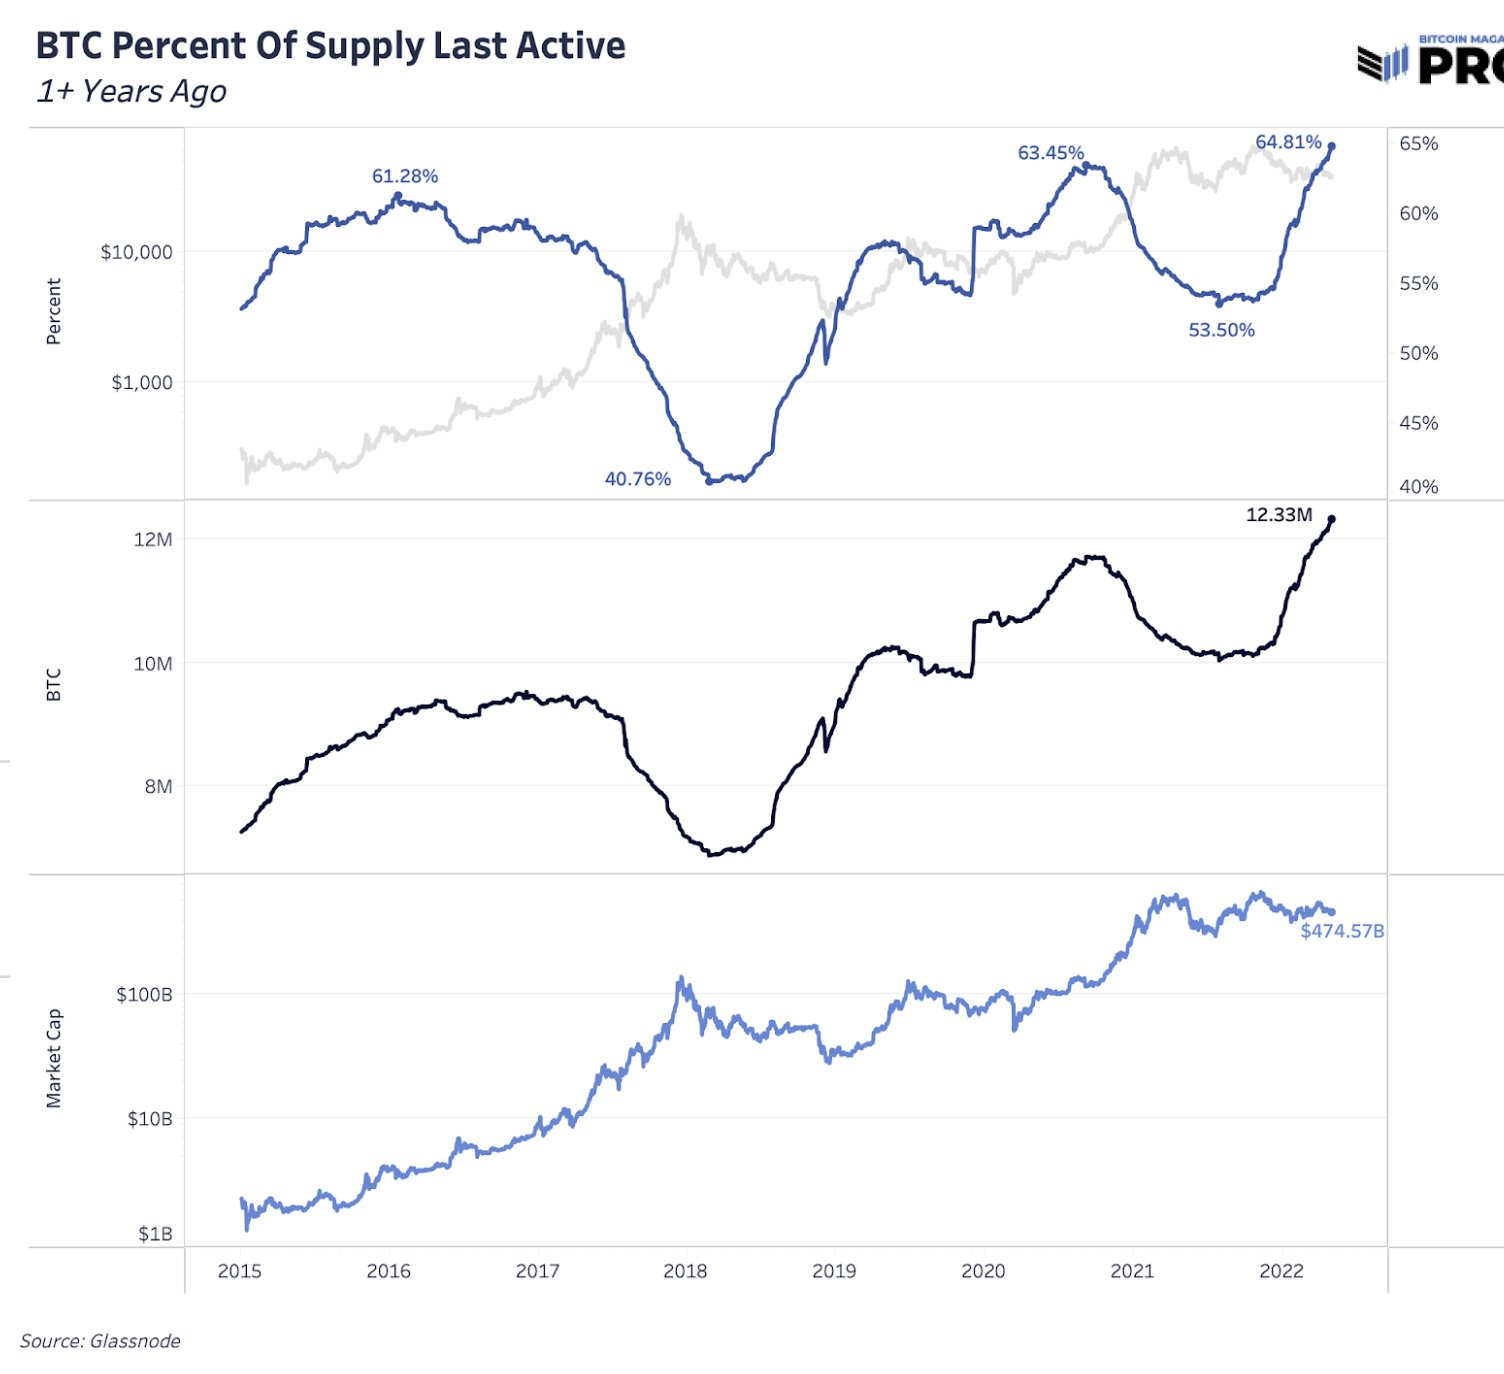
\includegraphics[width=0.5\linewidth]{notselling}
  \caption{Supply of bitcoin that hasn't moved for over 1 year}
  \label{fig:notselling}
\end{figure}
There's real recalcitrance about using the asset as a money, which leads to:
\subsubsection{Reduction of funding source / liquidity in legacy finance}
In the current financial system remuneration for labour performed in the workforce is loaned into the money system, where it's put to work providing liquidity for creation of more opportunity. This system actually works pretty well. The more of this deferred labour that's taken out of the legacy system, the less work can be done with what remains. This isn't to say that Bitcoin will cause a liquidity crisis, but there is possibly a cost if the current trend continues. This isn't as bad as:
\subsubsection{Bitcoin collapse system shock}
In the event of an existential collapse of the Bitcoin network the erasure of so much capital would certainly have a contagion effect on the whole global financial system. It's hard to imagine what such an event could be, this being the nature of ``black swans''. One cited example is the unravelling of cryptography by quantum computing. Some conspiracy theorists in the past have even speculated that Bitcoin is itself a canary in the coal mine, engineered by the NSA to warn about emergent quantum computing somewhere in the world. It's all pretty silly because without cryptography Bitcoin would be the least of humanities problems. The risk of `something' does exist though. The same anti-fragile feature can't be said about the technologies around Bitcoin, which gives us:
\subsubsection{Stablecoin collapse system shock}
This is much more likely. Stablecoins are under regulated, centralised, under collateralised, ponzo like structures, which could quite clearly fall apart at any point. The contagion effects of this are unclear as they're not yet too significant. They're a risk nontheless, and may be an indicator of:
\subsubsection{Tech for techs sake yielding unexpected outcomes}
The whole question of what Bitcoin addresses, whether it's been properly thought about, what the end goals are, and what the risks are is significant. It's a computer science and engineering solutions gone completely wild. It's clearly got benefits and there's clearly human appetite for this technology, but it's probably running ahead of the knowledge base around it. This is most exemplified in:
\subsubsection{No agreed measurable end goal}
 Bitcoin is a game theoretic juggernaut, where success of the network breeds more success for the network. The was obviously a great design choice for the computer scientists trying to solve the problem of a secure, and scalable, electronic cash, which couldn't be confiscated. Ironically for a global consensus mechanism it seems that nobody wants to discuss what constitutes a successful end point to this, and especially not what `successful' endpoints for the game theory which have calamitous negative repercussions for wider society look like.  This might have implications for:
\subsubsection{National security / actual warfare}
There's some national security implications for Bitcoin which are discussed both in the \href{https://twitter.com/JasonPLowery/status/1512775981693648897?}{fringes} and the \href{https://www.coindesk.com/layer2/2022/04/04/why-bitcoin-mining-is-a-matter-of-national-security/}{sector media}. Essentially, the industrial mining complexes which are more commonplace now, are easily identifiable targets, and provide nations with both some leverage over the global network, and a considerable source of income. The IMF correctly identifies these facilities as a way for nation states to \href{https://www.imf.org/en/Publications/GFSR/Issues/2022/04/19/global-financial-stability-report-april-2022}{monetise their energy reserves} without the need for foreign markets, opening the door to sanction avoidance. In the case of smaller and developing nation states who are perhaps subject to financial penalties on the global stage for whatever reason, these facilities start to look like legitimate targets for cyber and conventional warfare. This `weaponisation' of a neutral technology is already manifest in:
\subsubsection{Bitcoin as a culture war foil}
Bitcoin's online community skews very hard toward right wing libertarianism. This isn't to say there are no other voices, but they are certainly outnumbered. This imbalance is almost certainly a product of the ESG concerns around the technology. There has been a notable increase in diversity of thought since the evolution of the energy narrative, but it persists. This leads to a paucity of voices in policy making circles, and in the USA a strong delineation between policy makers along party lines. This kind of thing tends to be self reinforcing, and it seems very possible that the global liberal left will swing mainly against the technology, while the neoliberal right will be attracted more to it. As tensions increase so it seems does the online rhetoric. Even scientists now seem to agree that Bitcoin investors are calculating psychopaths \cite{martin2022dark}. This leads to:
\subsubsection{Self reinforcing monocultures}
There are some powerful `pockets' of fringe thinking within the vocal, online, Bitcoin communities. The most palatable of these are figures like Elon Musk and Jack Dorsey, but there's whole subcultural intersections around antivax, anti-woke, anti cancel culture, and fad diets. It might seem that this isn't terribly important, but Bitcoin viewed though the lens of these of these communities looks pretty strange to the newcomer. The early adopters are just using their wealth to leave the battlefield behind using:
\subsubsection{Jurisdictional / legislative  arbitrage}
The reach of Bitcoin and it's ability to undercut the global money systems, delivering savings for those with a first mover advantage, and the current paucity of agreed legislation has set up an interesting and rare condition. Bitcoin encourages something called jurisdictional arbitrage; the race to take advantage of the variance in national approaches to the asset class. This section could perhaps be explored as a list of opportunities, but from the viewpoint of our SME business use case it's far more likely that these destabilising `features' are risks.\\
\textbf{Capital gains tax avoidance}\\
Which is trivial, because countries are now competing to offer zero tax as a way to attract valuable tech mind share. They don't care if they never see a share of the profits earned elsewhere in the world.\\
\textbf{Income tax}\\
The same is true of income tax which is variously pitched around the world. It's hard to monitor this stuff and tax at source like with company employees wages, because it's basically designed to be hard to monitor. This results in:\\
\textbf{Passport perks}\\
There's a lot of new ways to buy passports and citizenship based on `inclusion' in this community now. It's a terrible look. The early adopters can live international jetsetter lifestyles while the newcomers are subject to:
\textbf{KYC/AML}\\
Currently there's a trend toward globally capturing information about people buying these assets, but it's effectively tech warfare now with engineers, rapidly producing tools to circumvent slow and varied legislation. The best example of this remains El Salvador, where Bitcoin is legal tender, and has perhaps kickstarted:\\
\textbf{Bond issuances}\\
El Salvador are having a \href{https://www.ft.com/content/4fa63c8c-51f5-4512-b522-76dd75e62916}{faltering start} to their promised bond issuance.\par
\href{https://prospera.hn/news/press-releases/pr\%C3\%B3spera-announces-bitcoin-bond-authority-in-the-first-crypto-friendly-jurisdiction-that-is-fully-aml-kyc-compliant}{Prospera}\\
\textbf{Trading fees tax variance}\\


\textbf{Business subsidies}\\
Again \href{https://davisclute.medium.com/visiting-a-startup-city-in-honduras-73d9c026ee6d}{Prospoera}
\subsubsection{Hyperbitcoinization}
Hyperbitcoinization is a term coined in 2014 by Daniel Krawisz \cite{krawisz2014hyperbitcoinization}. It is the hypothetical rise of Bitcoin to become the global reserve currency, and the demonetisation of all other store of value assets. This seems unlikely but is hinted at in a game theoretic analysis of both Bitcoin and current macro economics. Again, Bitcoin is a likely very poor replacement for money. The ability to monetise assets through banks, backed by law and contracts (the debt based system), is a highly refined human concept, while Bitcoin is a fusion of Austrian economics, and a computer science project. Malherbe et al. point out the inherent unsuitability of a deflationary asset such as Bitcoin as the global reserve currency \cite{malherbe2019cryptocurrencies} and feel that perhaps other cryptocurrencies might be more suitable for adoption by governments.  Interestingly this is the only paper to reference `Duality'.\par  Fulgur Ventures (a venture capital firm) provide a \href{https://medium.com/@fulgur.ventures/the-roads-to-hyperbitcoinization-part-1-27dc84d0e5e5}{blog post series} about the route this might take. It's important to note that Budish suggested that the usefulness of Bitcoin (and blockchain) cannot exceed the cost to attack it. The is highly suggestive that hyperbitcoinisation is impossible \cite{budish2018economic}. It's beyond the scope of this book to look at the implications of all this. 

\section{Does DeFi matter to SMEs }
DeFi is decentralised finance, and might only exist because of partial regulatory capture of Bitcoin. If peer-to-peer Bitcoin secured yield and loans etc were allowed then it seems unlikely that the less secure and more convoluted DeFi products would have found a footing. DeFi  has been commonplace over the last couple years, growing from \href{https://a16zcrypto.com/state-of-crypto-report-a16z-2022/}{essentially zero to \$100B} over the last two or three. It enables trading of value, loans, and interest (yield) without onerous KYC. If Bitcoin's ethos is to develop at a slow and well checked rate, and Ethereum's ethos is to move fast and break things, then DeFi could best be described as throwing mud and hoping some sticks. According to a recent JPMorgan industry insider report, around 40\% of the locked value on the Ethereum network is DeFi products. It is characterised by rapid innovation, huge yields for early adopters, incredibly high risk, and a culture of speculation which leads to products being discarded and/or forked into something else in the pursuit of returns.\par 
Much of the space is now using arcane gamification of traditional financial tools, combined with memes, to promote what are essentially pyramid schemes. Scams are very commonplace. Loss of funds though code errors are perhaps even more prevalent.\par
The Bank for International Settlements have the stated aim of supporting central banks monetary and financial stability. Their \href{https://www.bis.org/publ/qtrpdf/r_qt2112b.pdf}{2021 report on DeFi} noted the following key problems.
\begin{itemize}
\item ..a ``decentralisation illusion'' in DeFi due to the inescapable need for centralised governance and the tendency of blockchain consensus mechanisms to concentrate power. DeFi`s inherent governance structures are the natural entry points for public policy.
\item DeFi’s vulnerabilities are severe because of high leverage, liquidity mismatches, built-in interconnectedness and the lack of shock-absorbing capacity.
\end{itemize}
These are two excellent and likely true points. In addition access to DeFi is `usually' through Web2.0 centralised portals (websites) which are just as vulnerable to legal takedown orders as any other centralised technology. Given who the major investment players seem to be in this `new' financial landscape it seems very likely that regulatory capture is coming. The seemingly unironic trend towards CeDeFi (\href{https://www.nasdaq.com/articles/cedefi-what-it-is-and-why-it-matters}{centralised decentralised finance}) illustrates this; it's is all likely a fad.\par
There are more recent DeFi on Bitcoin contenders, but these are vulnerable to the \href{https://bisq.community/t/trading-halted-until-v1-3-0-hotfix/9208}{same attacks} and problems in the main. \par 
There is likely no use for this technology for small and medium sized companies on the international stage. It is far more likely that reputation would be damaged. The `best' of the portfolio of DeFi offerings is perhaps high yield stablecoin accounts, where dollars equivalent tokens are locked up providing very high return rates of up to 20 percent. It's also possible to get loans (by extension business loans) out of such systems at relatively low risks. The best `distributed' example of this is probably \href{https://lend.hodlhodl.com/}{Lend, at HODLHODL}, which is a peer-to-peer loan marketplace. \href{https://atomic.finance/blog/a-laypersons-guide-to-discreet-log-contracts-atomic-yield-series-part-3/}{Atomic Finance} leverages \href{https://adiabat.github.io/dlc.pdf}{discrete log contracts} amongst other more edge uses of Bitcoin, to provide financial services without custody of the users' Bitcoin. It is possible to make the argument that between hodlhodl loans, taro asset issuance, boltz exchange, and lightning escrow that all of the ``classes'' of DeFi smart contract can be serviced already by Bitcoin alone.\par
Many more custodial options exist for loans (CASA, BlockFi, Nexo, Ledn, Abra etc). These might not really fit the definition of DeFi at all, but they are potentially useful to companies who have Bitcoin on their balance sheet long term. Dan Held maintains an \href{https://docs.google.com/spreadsheets/d/1ZoapTCl76wahFMeNISSx9UdC3QBx-zC_jY4Le1H5Sdg/htmlview#}{online spreadsheet} which compares these products.\par
\section{Do DAOs matter to SMEs}
A DAO is an organistion which is built in distributed code on a blockchain smart contract system. Token holders have voting rights proportional to their holding. The first decentalised autonomous organisation was simply called ``The DAO'' and was launched on the Ethereum network in 2016 after raising around \$100M. \href{https://www.gemini.com/cryptopedia/the-dao-hack-makerdao#section-what-is-a-dao}{It quickly succumbed to a hack and the money was drained}. This event was an important moment in the development of Ethereum and resulted in a code fork which preserves two separate versions of the network to this day, though one is falling into obsolescence. \\
In practice DAOs have very few committed `stakeholders' and the same names seem to crop up across multiple projects. Some crucial community decisions within large projects only poll a couple of dozen eligible participants. Its might be that the experiment of distributed governance is failing at this stage. \\
Perhaps more interesting is the use of the DAO concept to crowd fund global projects, currently especially for the acquisition of important art or cultural items. DAOs are also emerging as a way to fund promising technology projects, though this is reminiscent of the 2017 ICO craze which ended badly and is likely to fall foul of regulations.\\
Within the NFT and digital art space  PleaserDAO has quickly established a strong following.
``PleasrDAO is a collective of DeFi leaders, early NFT collectors and digital artists who have built a formidable yet benevolent reputation for acquiring culturally significant pieces with a charitable twist.\\
Opensea wrangle between IPO and governance token.\\
ConstitutionDAO, Once upon a time in Shaolin etc 
%https://harpers.org/archive/2015/01/come-with-us-if-you-want-to-live/


\chapter{Distributed Autonomous Organisations}
A DAO is an organistion which is built in distributed code on a blockchain smart contract system. Token holders have voting rights proportional to their holding. The first decentalised autonomous organisation was simply called ``The DAO'' and was launched on the Ethereum network in 2016 after raising around \$100M. \href{https://www.gemini.com/cryptopedia/the-dao-hack-makerdao#section-what-is-a-dao}{It quickly succumbed to a hack and the money was drained}. This event was an important moment in the development of Ethereum and resulted in a code fork which preserves two separate versions of the network to this day, though one is falling into obsolescence. \\
In practice DAOs have very few committed `stakeholders' and the same names seem to crop up across multiple projects. Some crucial community decisions within large projects only poll a couple of dozen eligible participants. Its might be that the experiment of distributed governance is failing at this stage. \\
Perhaps more interesting is the use of the DAO concept to crowd fund global projects, currently especially for the acquisition of important art or cultural items. DAOs are also emerging as a way to fund promising technology projects, though this is reminiscent of the 2017 ICO craze which ended badly and is likely to fall foul of regulations.\\
Within the NFT and digital art space  PleaserDAO has quickly established a strong following.
``PleasrDAO is a collective of DeFi leaders, early NFT collectors and digital artists who have built a formidable yet benevolent reputation for acquiring culturally significant pieces with a charitable twist.\\
Opensea wrangle between IPO and governance token.\\
ConstitutionDAO, Once upon a time in Shaolin etc 
%https://harpers.org/archive/2015/01/come-with-us-if-you-want-to-live/


\chapter{Distributed Self Sovereign Identity}
%\section{Notes and thoughts - to be completed}
This chapter is an oddity because most of traditional DID/SSI isn't really fir for purpose. Distributed self sovereign identity has a great elevator pitch though. Individuals should be empowered through technology to manage their own data, without manipulation or exploitation by centralised corporate behemoths. In practice it's a staggeringly complex proposition which increases risk to the individual, decreases convenience, and despite much work, does not even make much sense in it's own terms. Webs of trust are viable so this means Nostr, \href{https://github.com/project-bitmark/marking/wiki#marking}{Marking}, or Slashtags which will be discussed, but are early products. %Maybe LNURL-Auth can do it. \par 
Thanks to \href{https://github.com/melvincarvalho}{Melvin Carvalho} for advice with this section.
\section{Applications of DID/SSI}
Some of the likely, and discussed applications for DID/SSI are the more inherently private and personally valuable sets of data a individual might generate throughout their life. The theory is that subsets of such data could then be digitally revealed by the individual when required, and that cryptographic verification built into the system would guarantee the veracity of the data to the receiving party. It is also possible to make use of ``zero-knowledge proof'' such that assertions can be made about about the contents of the data without revealing the data itself. A good example of this an age verification challenge, where a threshold age could be asserted without necessarily revealing the date of birth. 
Other keystone uses of the technology are:
\begin{itemize}
\item health documents history
\item qualifications and certifications
\item financial record and relationships with those of others
\item contacts, connections to other people and their appropriate data, including things like shared and personal calendars
\end{itemize}  
It's also possible to extend this key management ethos to all login credentials, and all data currently stored on centralised servers. This is the tension discussed in the chapter about Web3. Proponents think that using something like a DID/SSI stack to manage encryption, decryption and access to data within cloud services gives the user the best of all worlds. They see simply logging in with a cryptographic wallet, and using that same public/private key pair to manage the data beyond as some kind of panacea. This is very complex stuff though, and it seems very likely they just haven't thought this through enough.
\section{Classic DID/SSI}
Distributed identity / self sovereign identity has been extensively researched for decades, with hundreds of peer reviewed papers, and extensive support from the \href{https://www.w3.org/TR/did-core/}{world wide web consortium}. The academic field now seems quite ossified and has settled on a couple of hundred `schema' which they feel underpin the next layer of development. It is a \href{https://medium.com/decentralized-identity/overview-of-decentralized-identity-standards-f82efd9ab6c7}{complex field}, and the language and diagrams are arcane and self referential as seen in Figure \ref{fig:DID}.
\begin{figure}
\includegraphics[width=\linewidth]{DID}
  \caption{Part of the DID SSI specs}
  \label{fig:DID}
\end{figure}. 
Moreover the minimal implementation of such proposed systems hints at a \href{https://www.w3.org/community/perma-id/}{federated model} of centralised `truth' to enable persistence of identifiers over time.\\
The major failing of the DID/SSI work to date is a lack of meaningful use cases with incentives for adoption. This is clearly explained by Lockwood \cite{lockwood2021exploring} who proposes that the pathway to adoption of `classic' DID/SSI requires an incentive over and above the current identity management on the web. Being distributed is not enough. Especially in the light of questionable assurances of this even being true.\\
Perhaps most concerning is this \href{https://lists.w3.org/Archives/Public/public-credentials/2022Mar/thread.html}{recent exchange} on the mailing lists. Here, the two inventors of DID say the following:\\
\textit{``Not a single entity I know that's doing production deployments has actually vetted did:ion and found it to be production capable. This goes for every DLT-based DID Method out there - even the one we're working on. I am highly sceptical of anyone that says that any DID Method is ready for production usage at present.\\
Agreed — as one of the proponents of DLTs (in particular permissionless public ones) none are mature enough yet for production.''}.
It seems then that we can rule out use of these technologies?

\subsubsection{DID principles}
The core principles of distributed identity are that there should be persistent identifiers, like real world documents which assert identity, but with extended use cases. These should be permanent, and resolvable everywhere, forever. Underpinning this is cryptographically verifiable and decentralised data, managed by the user, or their trusted proxy. As primitives this makes them lifetime digital assets, that are portable, and unconfiscatable, with no required reliance on a trusted third party. By this stage in the book you should be familiar with these concepts, but application of this fundamental mindset to all personal data and digital interactions is a bigger reach even than money and value.
\subsubsection{What's in a DID document?}
All classic DID is underpinned by a DID document what bootstrap the services it's connected to. It is made up of one or more public keys. The documents can make use of services such as timestamps, cryptographic signatures, proofs, delegations, and authorisations. They should contact the minimum about of information to accomplish the specific task required of them.

\section{Newer Technologies}

modelling reputation diagram 2.3.2 \cite{mui2002computational}

\subsection{Slashtags}
Slashtags is a new distributed identity open method being developed by Bitfinex and Tether under the Synonym suite. It uses Bitcoin keys for authentication, but communicates a schema through a metadata exchange.
\subsection{Microsoft ION}
While working at Microsoft on ION Daniel Buchner (now working at Square) or Henry Tsai \href{https://github.com/decentralized-identity/ion/blob/master/docs/Q-and-A.md}{said the following}, which is worth quoting verbatim:\par
``While ledger-based consensus systems, on the surface, would seem to provide the same general features as one another, there are a few key differences that make some more suitable for critical applications, like the decentralized identifiers of human beings. Some of these considerations and features are:
\begin{itemize}
\item The system must be open and permissionless, not a cabal of authorities who can exclude and remove participants.
\item The system must be well-tested, and proven secure against attack over a long enough duration to be confident in.
\item The system must produce a singular, independently verifiable record that is as immutable as possible, so that reversing the record the system produces is infeasible.
\item The system must be widely deployed, with nodes that span the globe, to ensure the record is persisted.
\item The system must be self-incentivized, so that nodes continue to operate, process, and secure the record over time. The value from operation must come from the system directly, because outside incentive reliance is itself a vector for attack.
\item The cost to attack the system through any game theoretically available means must be high enough that it is infeasible to attempt, and even if an ultra-capitalized attacker did, it would require a weaponized mobilization of force and resources that would be obvious, with options for mitigation.\par

The outcome:

\item Number 1 eliminates private and permissioned ledgers
\item Number 2 eliminates just about all other ledgers and blockchains, simply because they are inadequately tested
\item For the metrics detailed in 3-6, Bitcoin is so far beyond all other options, it isn't even close - Bitcoin is the most secure option by an absurdly large margin.''
\end{itemize}

On the surface then it might seem that the choice is Bitcoin again, and indeed that the open source Microsoft ION stack is a natural choice, but it's complex to run, the interactions with the blockchain have a cost implication which can't be surmounted without every user owning some Bitcoin, and as we have seen, there is no formal validation of this system. It seems that it might be somewhat useful `at scale' and is worth consideration.
\subsection{Nostr}
Nostr is ``The simplest open protocol that is able to create a censorship-resistant global "social" network once and for all.'' according to it's \href{https://github.com/fiatjaf/nostr}{github page}. More than that it's a client side validated proof of who a user is interacting with, hence being in this identity section. To be clear, it's not a completely peer to peer system in that it uses relay servers, but this gives it some of the best characteristics of both paradigms. This has the following advantages for our metaverse application; 
\begin{itemize}
\item it's lightweight, with minimal network overhead and complexity
\item it's real-time using websockets
\item anyone can run a relay server, so one can be run in the deployment in the final section of the book.
\item Each of the client peers connecting to the metaverse can be a relay and able to pass messages and proofs to the other clients without the metaverse server seeing the data or being online 
\item it's opensource
\item there are multiple usable libraries and tools
\item it's under active development with an excellent team. The lead, `Fiatjaf' is one of the most \href{https://github.com/fiatjaf}{prolific developers} in the lightning space.
\item it's based on the same underlying cryptographic technology we are using elsewhere, indeed the with it's use of Bitcoin keys the identity system is global
\item it provides the identity proof that we need to validate users and objects into a virtual space
\item it enables message passing
\item it scales to be a social network as required
\item it need not rely on anything outside of a relay hosted on the metaverse server
\item it can likely be scaled to provide one to many bulletin board style applications within the metaverse
\item it can easily operate outside of the walled garden of the metaverse, extending the reach of the messages
\end{itemize} 
Nostr is incredibly promising, and integrating these relays in the metaverse servers and clients of the proposed technology stack in this book might allow us globally provable identity, with privacy by design. It can provide message passing. If all entities in the metaverse scenegraphs are also Nostr key pairs then schema can be applied consistently with the economic layer using the same key system as Bitcoin. A curated list of projects and libraries is \href{https://github.com/aljazceru/awesome-nostr}{available on github}.
%\textbf{The proposed integration of Nostr, LnBit, Vircadia, and Bitcoin is the secret sauce of this book}. 
\section{Micropayment based web}
It seems the war against disinformation is now being lost. Much is written in the media about Deepfake technology creating plausible fake videos, but probably more pernicious is the use of toolkits to create entire plausible fake news sites using natural language AI such as GPT3. This makes it cheap to publish potentially market moving news which is then rehypothecated by online news vendors who are hungry for clicks. As these pipelines become more mature it will be difficult to keep fake news for financial or political gain out of the system. One interesting way to do this that \textit{isn't} webs of trust or true cryptographic identity is to charge micropayments for ``one to many'' publication models. This would imply a tiny instant payment for clicks, especially on social media sites such as twitter. This kind of model has been discussed but is only possible in the context of systems such as Lightning where instant micropayment can be realised. It seems possible that this would price out speculative `noise' spam from the information space. It's interesting and ironic that the origin of proof of work was to underpin just such a spam defeating system, and that Nakamoto \href{https://www.metzdowd.com/pipermail/cryptography/2009-January/015014.html}{mentioned this application for Bitcoin} back in 2009. There is now much chatter about the integration of Bitcoin with Twitter in light of Musks buyout of the social network.
%\subsection{Open World assumption}
%\href{https://en.wikipedia.org/wiki/Open-world_assumption}{this needs unpacking}
%------------------------------------------------
\section{Risks \& Challenges?}
Classic DID/SSI risks fragmentations
In all DID scaling to a world where the user is managing potentially thousands of these critical cryptographic data files is daunting.
Abstracting the guts of this away to make the user simple, and only caring about right level of information, turns out to be huge problem that nobody has solved
It's not clear that users want this
In the case of web of trust like Slashtags it's a big piece of work for the users to rate off of their digital interactions with a trust metric.




\chapter{Non Fungible Tokens}
Nonfungible tokens are a whole `class' of digital token, separate and distinct from everything discussed to this point. They are generally \href{https://www.signaturelitigation.com/nfts-recognised-as-property-lavinia-deborah-osbourne-v-1-persons-unknown-2-ozone-networks-inc-trading-as-opensea/}{recognised in law} as property in their own right \cite{moringiello2021property, fairfield2021tokenized}. In the Initial Coin Offering (ICO) and project tokens detailed earlier, and limiting this description of the Ethereum network for now, a project launching an ERC-20 token commits contract code to the blockchain, and this contract then mediates the issuance and management of million or billions of tokens associated with that project, and it's use case. \href{https://ethereum.org/en/developers/docs/standards/tokens/erc-20/}{ERC-20} is a \href{https://en.wikipedia.org/wiki/Fungibility}{fungible} token issuance. Each of the projects' tokens is interchangeable with any other token. They're all the same from the point of view of the user.\par
Rather than the ERC-20 contract type used for fungible token issuance NTFs predominantly use ERC-721 on Ethereum. It's the case that most NFTs in the current hype bubble are algorithmically generated sets of themed art (so called PFP-NFT). Tens of thousands of distinct tokens are `minted', each one being a complex transaction commitment to the Ethereum blockchain, along with it's associated gas fee. These minting events are much hyped social occasions, and happen very quickly, with users clamouring to create art with randomly allocated features from the art schema associated with the project. Lucky winners can find themselves with an NFT art piece with more than an average number of `rare' features. If the overall mint becomes more popular, then the secondary market for all of those mints goes up, and because of the liquidity premium they can go up a lot. The perceived rarer mints go up a lot more. This whole process is \href{https://memoakten.medium.com/the-unreasonable-ecological-cost-of-cryptoart-2221d3eb2053}{very energy intensive} on the chain, and the vast majority of these project simply \href{https://www.turing.ac.uk/blog/non-fungible-tokens-can-we-predict-price-theyll-sell}{trend to zero value}. \par
In response to this appalling cost benefit analysis the Ethereum foundation have proposed \href{https://eips.ethereum.org/EIPS/eip-2309}{EIP-2309} to make minting NFTs more efficient. They say ``This standard lets you mint as many as you like in one transaction!''\par
The Ethereum foundation give their somewhat constrained view of \href{https://ethereum.org/en/nft/}{NFTs on their website} and it's a useful primer. On that page they detail some of the use cases, as listed below with a critique added:
\begin{itemize}
\item Digital content; this is the dominant use case right now. Much more on this later.
\item Gaming items; again more on this later, it's an obvious enough use case but \href{https://climatereplay.org/nfts/nft-digital-ownership-pledge/}{complex politics} in the intersection of games and crypto have stalled the adoption curve
\item Domain names; this is just starting to reach for applications now, why not a database with the ISP/host?
\item Physical items; this is a clear over-reach as transfer of the NFT does not imply tranfer of the object.
\item Investments and collateral; while this is indeed an emergent option in the tech right now it's likely just a bubble, as owners of the tokens cast around for additional liquidity, and loan businesses chase yield with higher risk.
\end{itemize}
Moving away from Ethereum, NFTs can be minted on most of the other level one chains. Solana is a great newcomer example. Sol is a terrible chain with regards to decentralisation, but thanks to that it's far cheaper and faster to mint NFTs on it, and it's become a \href{https://markets.businessinsider.com/news/currencies/ethereum-eth-killers-nfts-defi-solana-cardano-wax-crypto-investing-2022-1}{troubling competitor} for Eth (Figure \ref{fig:solnfts}).\par 
\begin{figure*}[ht]\centering % Using \begin{figure*} makes the figure take up the entire width of the page
	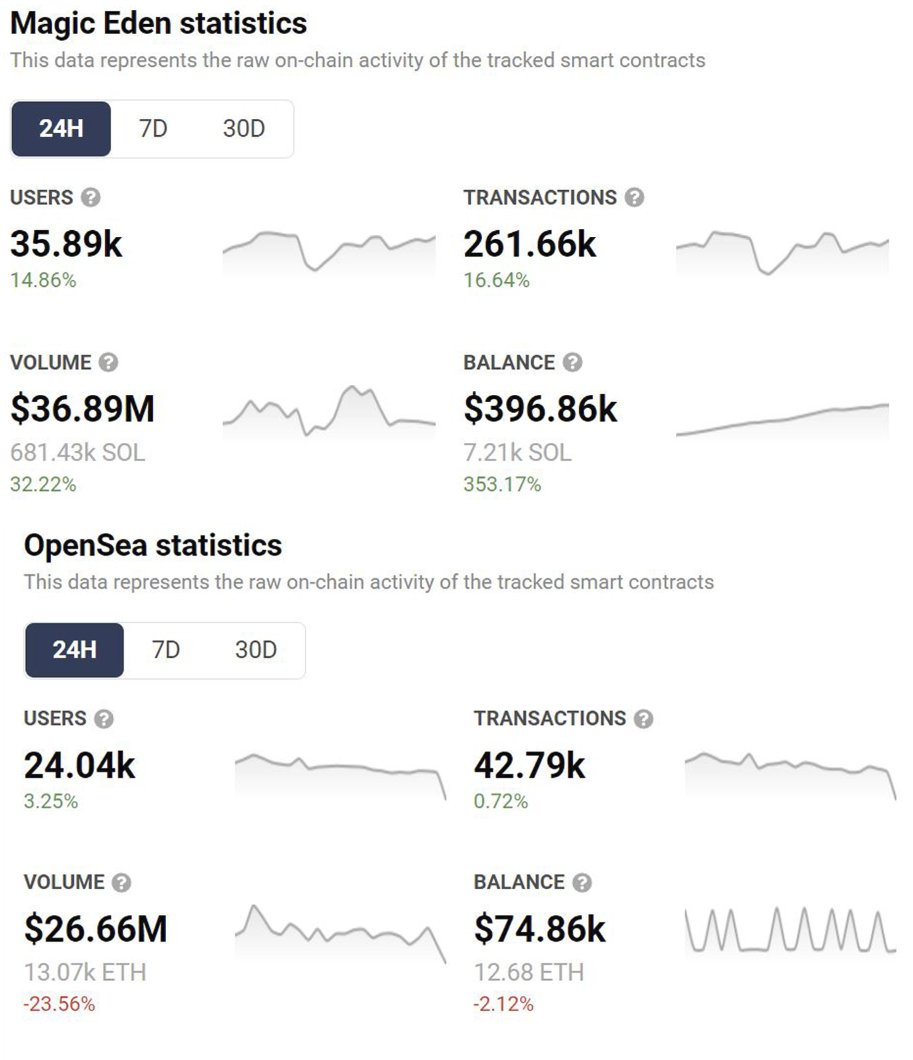
\includegraphics[width=0.7\linewidth]{solnfts}
	\caption{Solana NFT markets are enjoying growth compared to Opensea on Ethereum, even in the downturn.}
	\label{fig:solnfts}
\end{figure*}
The same might be true for Cardano's ADA, though ADA is struggling to hold onto it's market position despite some technical advances. It's worth reiterating here that the nature of these digital tools likely makes for a `winner take all' market dynamic over time. With fees being central to this generative NFT use case it's possible to see that highly centralised, fast, and cheap chains will capture and eventually dominate the space. Remember that this likely game theoretic outcome is a huge cognitive dissonance as this might as well be a database running without the stark inefficiencies of blockchain. The whole NFT space is a gamble on consumer enthusiasm for spending money continuing to outpace logic.\par 
Astonishingly, according to a JPMorgan insider market report (\href{https://www.coindesk.com/podcasts/the-breakdown-with-nlw/jpmorgan-bitcoin-shows-some-merit-as-a-store-of-value/}{reported on in a podcast}), only around 2 million people have ever actually interacted with NFTs. This is far below what one might expect given the hype.\par
With that said NFTs have clearly allowed \href{https://en.wikipedia.org/wiki/List_of_most_expensive_non-fungible_tokens}{digital and new media artists} to connect with audiences without gatekeepers. Established mediators and curators of art have been caught totally wrongfooted, and NFTs seem to give a way for them to be cut out completely. There are suggestions of applications beyond this initial digital art scope. This is a compounding, and disrupting paradigm change.\par
%Users of NFT markets have \href{https://blog.chainalysis.com/reports/nft-market-report-preview-2021/}{injected around \$30 billion into the tokens during 2021}. 

\section{Digital Art}
\textbf{NFT Use Cases}

\textbf{Art}

The recent surge of interest in NFT's during early 2021 has largely been
driven by digital art NFT's, despite the origins of digital art NFT's
started much earlier in 2014. New York artist
\href{https://www.mccoyspace.com/project/125/}{Kevin McCoy's
\emph{Quantum}} is widely recognised as the first piece of art created
as an NFT. However it was during early 2021 that art NFT's started to
gain significant attention; by the end of 2021, nearly
\href{https://www.paymentscardsandmobile.com/state-of-the-blockchain-nfts-explode-onto-scene-in-2021/}{£31b
had been spent} on NFT purchases, a considerable and exponential growth
given
\href{https://raritysniper.com/news/nfts-exploded-in-2021-with-25-billion-in-sales/}{2020
sales of \textasciitilde£71m}

High profile digital artists such as \emph{Beeple} whose
\href{https://www.forbes.com/sites/abrambrown/2021/03/11/beeple-art-sells-for-693-million-becoming-most-expensive-nft-ever/?sh=3f237d1c2448}{recent
recording break sale} of his NFT \emph{``The first 5000 days''} (Figure \ref{fig:first5000days}) at Christies (a long established British auction house,
specialising in high profile precious work of art) for £52.9m helped
bring NFT's into the public spotlight and wider give them global
attention.

\begin{figure*}[ht]\centering % Using \begin{figure*} makes the figure take up the entire width of the page
	\includegraphics[width=\linewidth]{first5000days}
	\caption{Beeple: First 5000 days, \href{https://onlineonly.christies.com/s/beeple-first-5000-days/lots/2020}{taken from the Christies website, assumed fair use}.}
	\label{fig:first5000days}
\end{figure*}

Art as NFT's offer the following advantages:

\begin{enumerate}
\def\labelenumi{\arabic{enumi}.}
\item
  \textbf{Immutable Nominal Authenticity:} Art fraud such as false
  representation, forgeries, plagiarism have been a reoccurring blight
  since art has existed; artists and works of art have been open to
  abuse by forgers, black market profiteers and even fellow artists
  laying claim to works of art of others. Unless a work of art is sold,
  exhibited or listed, documenting when and who created it, the
  \emph{nominal authenticity,} which Dutton states as the
  \emph{``correct identification of the origins, authorship, or
  provenance of an object''} \cite{dutton2003authenticity} can be increasingly mutable over a period
  of time, dependent on a multitude of factors, including; the artists
  existing profile, how widely and where the work of art is exhibited,
  if the work of art is commissioned by a patron, if it's sold, and
  profile of the buyer/collector. At its most basic level, once a work
  of art is `minted' as an NFT (publishing the art work as a unique
  token on the blockchain) this functions as an immutable publicly
  accessible proof of ownership and by extension proof of creation. The
  act of minting is not purely limited to digital art; all an artist
  requires is a digital representation of any physical art (sculpture,
  physical painting, installation etc..) which can be used as a proxy
  allowing artists to record the date of creation/origin of a physical
  piece of art on the blockchain, a buyer purchasing the NFT can be
  provided the actual physical artwork as part of the NFT. Nominal
  authenticity becomes secure and immutable.

  \begin{enumerate}
  \def\labelenumii{\alph{enumii}.}
  \item
    \textbf{Secure Digital Provenance}:
    \href{https://en.wikipedia.org/wiki/Provenance}{Provenance} (or the
    chain of custody) is an important aspect in works of art, antiques
    and antiquities. Provenance not only helps assign work to an artist
    but also documents ownership history. Digital provenance, an
    inherent feature of NFT's means provenance now no longer becomes
    what has historically sometime been a contentious detective's game
    at the best of times; one that is open to fraud, misinterpretation
    and entirely reliant on good record keeping.
  \end{enumerate}
\end{enumerate}

\begin{quote}
Since provenance can contribute to the value of a piece of art
(benefiting both the creator and collector) the use of the blockchain as
an open, secure ledger is a far more trustworthy system than traditional
methods of artistic provenance that were cobbled together; often
consisting of a mix of physical and digital documents spanning private
\& public sale receipts, art/museum gallery exhibitions and private
record keeping). Digital provenance provided when an artist `mints' a
piece of art into an NFT allows artists and collectors to record a
secure, permanent unalterable history of transactions for a specific
piece of art, providing future collector complete trust in the origin
and custody of a piece of art.
\end{quote}

\begin{enumerate}
\def\labelenumi{\alph{enumi}.}
\setcounter{enumi}{1}
\item
  \textbf{Decentralised automated royalty payments}: Traditionally if a
  piece of art is sold, the first sale may (but not always) benefit the
  artist financially, however secondary and any subsequent sales would
  only ever financially benefit the buyer/collector; the original artist
  would rarely benefit. However If a work of art is minted into an NFT,
  royalty payments can be predetermined and automated in perpetuity
  directly by the use of a `smart contract'. Smart contracts are small,
  automated scripts/programs that run automatically and independently of
  a buyer/seller; pre-determined conditions are set by the buyer; these
  trigger when certain conditions are met i.e

  \begin{enumerate}
  \def\labelenumii{\roman{enumii}.}
  \item
    \emph{On sale transfer 20\% of total sale amount into digital wallet
    of the creator.}
  \item
    \emph{On sale transfer 80\% of total sale amount into digital wallet
    of the seller.}
  \end{enumerate}
\end{enumerate}

\begin{quote}
Once the royalty payment rate is set by the artist/creator, future
royalties of all sales can be paid directly to the artist/creator
account (via a digital wallet) without the need of a third party
(traditionally a gallery/agent etc..).

Smart contract driven NFT's means that even if piece of art is resold 5,
10 or even a 100,000 times moving through 5, 10 or even a 100,000
different collectors; a pre-determined royalty payment rate set by the
creator would still guarantee the artist/creator is paid directly from
each and every future sale.

Historically provenance for works of art may span across generations,
for instance Gabriël Metsu's oil on canvas painting \emph{The Lace
Maker's} provenance, first recorded in 1722, now spans 300 years of
ownership, including from a British Baron in the 19\textsuperscript{th}
century to an American philanthropist in the 20\textsuperscript{th}
century.) Metsu died young at the age of 38, leaving a widow; neither
his/her relatives/descendants benefit from his original work, 300 years
later this would be near impossible to facilitate with traditional
systems, as even legal contracts are open and prone to the ravages of
time.

NFT smart contracts hold an incredibly potential; an artists descendants
financially benefiting directly from the resale of a piece of work long
after the artist/museum's/gallery or even state have turned to dust as
long as the original creator's digital wallet is accessible, \emph{the
blockhain becomes an everlasting digital patron} ensuring
\end{quote}

\textbf{Computer \& Video Games}

Computer \& Video games are a huge global business, exponential global
growth over the last 30 years has seen this grow to a point where it has
eclipsed both the
\href{https://www.businessinsider.com/video-game-industry-revenues-exceed-sports-and-film-combined-idc-2020-12?r=US\&IR=T}{global
movie and North American sports industries} combined.

A global industry with revenues over £120b,
\href{https://www.wepc.com/news/video-game-statistics/}{with
\textasciitilde half the people on the planet} playing some form of
games in 2021.

As the games industry has evolved and matured over the last 40 years,
secondary markets have emerged, most notably the `second hand' games
resale market. The rise of `retro' gaming, has demonstrated the second
hand market is a lucrative one for private resellers, an unopened copy
of Super Mario Bros for the Nintendo Entertainment System
\href{https://www.nytimes.com/2021/08/06/business/super-mario-bros-sale-record.html}{recently
selling for £1.5M} to the extent the market has seen
\href{https://www.businessinsider.com/retro-gaming-market-being-overtaken-by-speculators-2021-9?r=US\&IR=T}{speculators
looking to cash in} on the huge global interest in retro/second hand
games

Despite publishers and developers increasingly moving to non-physical
digital only' games, the demand for used games remains incredibly high.

Whilst some retailers have adapted their business models to include
reselling of retro/second hand games, the vast majority of
publisher/developers/retailers aren't able to directly benefit from the
emerging retro/second hand games market. The potential of \emph{video
games as NFT's} presents a huge opportunity for publishers, developers
and players alike, offering the following advantages:

\begin{enumerate}
\def\labelenumi{\alph{enumi}.}
\item
  \textbf{Royalty Sales on Pre-owned Games} ; A predetermined proportion
  of any resale of a used game can automated in perpetuity via smart
  contracts; once these are set by the publisher, future royalties of
  all sales can be paid directly to the publishers/developers wallets (a
  digital account) without the need of a third party (traditionally a
  retail entity). Traditionally only the initial first sale of a game
  would financially benefit the publisher/developer/retailer, secondary
  and subsequent sales would only ever financially benefit the
  purchaser, with many developers/publishers arguing this is hurting the
  wider industry through the loss of significant income generated by the
  secondary and subsequent sales, sometimes over the course of decades.
  However the use of NFT's smart contracts means that if a game is
  sold/resold through 10,000 collectors; a pre-determined royalty
  payment rate set by the publisher would still guarantee the publisher
  (and or developer/retailer) takes a proportion of any future sales.
\item
  \textbf{Monetisation of User Generated Content:} Games as a NFT's
  offer ability to monetise UGC: User generated content.
\end{enumerate}

\begin{quote}
Video games such as
\href{https://www.businessofapps.com/data/pokemon-go-statistics/}{Nintendo's
\emph{Pokemon Go}} \emph{(166 million players)},
\href{https://techacake.com/destiny-2-player-count/\#:~:text=The\%20total\%20player\%20base\%20of,to\%20be\%2038\%20million\%20players.\&text=According\%20to\%20the\%20source\%2C\%20the,in\%20terms\%20of\%20player\%20population.}{Bungie's
\emph{Destiny 2}} \emph{(38 million players)} or
\href{https://fictionhorizon.com/how-many-people-play-genshin-impact/\#:~:text=Genshin\%20Impact\%20had\%20approximately\%209,million\%20users\%20in\%20June\%202021.}{miHoYo's
Genshin Impact} (\emph{9 million players} ) all have large, established
and significant player bases. What is noteworthy, the games are designed
to encourage players may spend hundreds, or in some cases thousands of
hours on one game alone; according to
\href{https://destinytracker.com/destiny/leaderboards/all/minutesplayedtotal?grouped=true\&page=1}{Destinytracker.com},
the top players have amassed total play times over 20,000 hours, close
to 1,000 days or \textasciitilde{} 3 years, which is incredible feat
given Destiny 2 only launched 5 years ago in 2017.

Destiny/Pokemon Go and Genshin Impact revolve around a central key game
mechanic; players investing significant amounts of time collecting in
game digital assets; characters/weapons/items, often classed as `rare'
or `exotic' or `5 Star'. These collectibles usually found by a
combination of the accrual of in-game time, completing quests,
purchasing additional in-game items/boosters, and luck (`RNG'). Players
are often encouraged to share their collections of rare
characters/weapons/ objects through in-game achievements, triumphs,
scores acting as a mark of distinction/status symbol.

Traditionally there has been nothing that went beyond sharing the
\emph{digital badge} (i.e triumph/achievement/accomplishment) on a on
social media/gamer's platform profile. However NFT's offer the ideal
system for developers/publishers and even players to monetise user
generated/customised data (such as a players unique save game data),
simultaneously allowing:

a) creation of an additional monetised ecosystem to meet player demands
i.e. some players who are willing to monetise and `sell' their invested
time in a particular product/service to other players with little time
but willing to pay other players for `grinding' (progressing laborious
in game tasks) and a more advanced in-game progression point.

The potential to provide publishers/developers with an additional
long-term income stream, providing a better ROI on computer \& video
game development, which in many instances can cost hundreds of millions
in development costs spanning 5/10 years, is undeniable.
\end{quote}

\begin{enumerate}
\def\labelenumi{\alph{enumi}.}
\setcounter{enumi}{2}
\item
  Play to earn revenue models, though this is morally dicey and early startups like \href{https://www.bloomberg.com/news/features/2022-06-10/axie-infinity-axs-crypto-game-promised-nft-riches-gave-ruin}{Axie Infinity are in serious trouble}. A (long) \href{https://www.youtube.com/watch?v=YQ_xWvX1n9g}{video by Dan Olsen} highlights the structural problems with both play to earn and NFTs.
\item
  Monetizing In game collectibles: customisable in game assets (vanity
  items such as cosmetic character skins/clothing or collectible items
  that offer player advantages(new weapons/vehicles/mods etc,..)
\end{enumerate}

\textbf{Figure 1.x:} Typical Smart Contract Structure:
https://www.jigsawllc.com/2021/03/25/nfts-creativity-innovation/

%\section{NFTs and games}
NFT art currently suffers from the same failure of decentralisation already discussed in the Ethererum technology stack, but this is compounded by the normalisation of intermediate art brokers \href{https://moxie.org/2022/01/07/web3-first-impressions.html}{continuing to custody} the NFTs even after sale. They are usually selling a pointer to their own servers. The market is nascent and evolving, but it's currently not delivering on it's core promise.\par
Proof of ownership is intuitively a pretty obvious application for the technology, but again it's hard to justify the expense when the benefits are so slim. \href{https://www.bullishlybred.com/}{Bulldogs on the blockchain} is a clear gimmick, and might even incentivise poor behaviours as there are two products here which are not necessarily aligned. Much has been written over the years about \href{https://propy.com/browse/propy-nft/}{deeds to property} being passed through blockchains, cutting out the middle man, but in the event that a house deed NFT was hacked and stolen it's obviously not the case that the property would then pass to the hacker.
While it is likely that this is currently a speculative bubble, that is \href{https://www.bbc.co.uk/news/business-61102759}{waning already} (Figure \ref{fig:monkey}), it seems certain that the technology is here to stay in some form.\par


\section{MMORG games and NFTs}
Traditional gamers have pushed back on the seemingly useful idea of integrating NTFs with traditional games. This may be in part because Ethereum mining has kept graphics card prices high for a decade.

\href{https://www.prnewswire.com/news-releases/hbar-foundation-and-ubisoft-partner-to-support-growth-of-gaming-on-hedera-network-301474971.html}{HBAR partnerships}\par
\href{https://finance.yahoo.com/news/epic-games-vp-people-have-lost-interest-in-the-metaverse-200725562.html}{Critique from Marc Petit of Epic and Unreal}.\par
The \href{https://twitter.com/justinkan/status/1491270239967154178}{following text} is from Justin Kan, co-founder of twitch: \textit{``NFTs are a better business model for games. Many gamers seem to be raging hard against game studios selling NFTs. But NFTs are also better for players. Here’s why I think blockchain games will be the predominant business model in gaming in ten years. NFTs are a better business model for funding games . Example: recently I invested in a new web3 game SynCityHQ. They are building a mafia metaverse and raised \$3M in their initial NFT drop.\\ NFTs give studios access to a new capital market for raising capital from the crowd.NFTs can be a better ongoing model for games. Web3 games will open economies, and by building the games on open and programmable assets (tokens + NFTs) they will create far more economic value than they could from any one game. Imagine Fortnite, but other developers can build experiences on top of the V-Bucks and skins. Epic would get a royalty every time any transaction happens. As big as Fortnite is today, Open Fortnite could be much bigger, because it will be a true platform. NFTs are better for gamers Allowing gamers to have ownership of the assets they buy and earn in game allows them to participate in the potential growth of a game. It lets gamers preserve some economic value when they switch to playing something new. But what about the criticisms of NFTs?\\
Here are my thoughts on the common FUDs: "It’s just a money grab on the part of the studios!"\\
Game studios already switched over to the model of selling in-game items, cosmetics, etc to players long ago. But currently the digital stuff players are buying isn’t re-sellable. NFT ownership is strictly better for players. "The games aren’t real games." This reminds me of the criticism of free-to-play in 2008, when the games were Mafia Wars / FarmVille. We haven’t had time for great developers to create incredible experiences yet. Everyone investing in games knows there are great teams building. "Game NFTs aren’t really decentralized because they rely on models / assets inside centralized game clients."
Crypto is as much a movement as it is a technology. Putting items on a blockchain is what gives people trust that they have participatory ownership...which make people willing to buy in to the game. These assets are “backed” by blockchain.
The fact that these item collections are NFTs will make other people willing to build on top of them. "NFTs are bad for the environment." Solana and L2s solve this. NFT games are better for players and for game developers. Like the free-to-play revolution changed gaming, so will blockchain. The games of the future will be fully robust, with open and programmable economies.}''
\section{Broader and metaverse uses}
So far according to a16z NFTs break down into:
\begin{itemize}
\item Profile pictures: These were discussed at the start of the chapter and have felt ubiquitous on Twitter over the last couple of years. The major projects will likely hold value, but the hype cycle will likely lead to all profile NFTs going in and out of fashion.
\item Art and Music: Art has also been discussed above. Peter Thiel, the billionaire venture capitalist who founded PayPal has invested in expanded NTF use cases. The first is `Royal' which is experimentally \href{https://royal.io/}{selling limited NFT tokens} which contractually entitle the holder to a portion of music artist royalties. Spotify are experimenting with music NFTs. This is an early adopter area.
\item Gaming: As discussed there's pushback from the gaming community, but huge investment from the likes of Lego, Blizzard, Epic, Ubisoft etc.
\item Gig tickets: Not only the straightforward use of transferable tickets for events as NFTs on a blockchain (which is impossible due to the cost right now) but also onward monetisation of ticket stubs as memorabilia. The NBA is \href{https://deadspin.com/investing-in-nft-ticket-stubs-is-likely-one-of-the-nba-1848991991}{already looking at this}.\\
\textit{``The team sells the ticket for face value many many years ago, but when that stub is being sold now for much more many times over, the team gets none of that money,'' York explained. ``But with an NFT stub that changes. Let’s say a new rookie enters the NBA next season and he turns out to be the next LeBron James. That ticket stub from his first game, as an NFT, the team can put a commission on it — 20 percent or however much, the NBA decides that. In 10 years when it’s worth a lot of money, I or whoever owns that NFT, can sell it for say \$100,000. The NBA can still collect 20 percent of that sale, because it’s all on a smart contract.''}
\item Utility: These are broadly `membership' style tokens, and this seems like a sensible fit. Peter Thiel (again) for instance launches a \href{https://www.ztonft.com/}{political funding NFT} from Blake Masters to support his senate ambitions. To be clear, Thiel is a fundamentalist libertarian, and at the very least \href{https://gizmodo.com/peter-thiel-bitcoin-talk-miami-2022-1848764790}{highly eccentric}. This is not necessarily a positive for the technology.
\item Virtual worlds are a huge application for NFTs, and this seems like it would be a natural fit for out metaverse application. In reality the \$2B of sold so far is mostly `allocations' in nascent ecosystems, being sold as highly speculative assets, without even a metaverse to use. The majority of that amount is the hyped `Otherland' plots sold under the Bored Apes brand.
\end{itemize}
It is completely reasonable to assert that these use cases could be accomplished without the use of NFT technology, and is part of the hype bubble.\par
Twitter user Cantino.Eth offers an exhaustive roundup of what these future uses might be. It's a \href{https://twitter.com/chriscantino/status/1542930648750608387}{thread full of industry insider jargon} but it's indicative of a shift in focus from speculation to `building' as the market conditions change. Some of the more interesting (less arcane) use cases identified in the thread are summarised very briefly below, with comments as to how this might pertain to our metaverse applications.
\begin{itemize}
\item Hobby tokens, demonstrating interest in an activity. This is potentially a metaverse adaptation of badges on a blazer in the real world, and might serve to drive communities in a metaverse. The same is true for activism and political alighnment. It's a great idea and worth developing.
\item Professional Networks and qualification badges, like a LinkedIn qualification panel, but in the metaverse. A cisco NFT in the metaverse for a CCNA qualification makes intuitive sense. 
\item Badges to indicate membership of distributed projects within a metaverse. This allows users to identify avatars with shared goals in the metaverse.
\item Retail incentives, like brand loyalty stamps or rewards for participation in marketing, or early access programmes. This is a true in a metaverse marketplace as it is in a real world coffee shop.
\item Multiplayer communities with incentives to hit collective milestones. ``Collectiing as a team sport''. This again seems like a great and intuitive opportunity, but is perhaps less suitable for our more business focussed space.
User content submission and automatic monetisation when reused by brands, bonded to an NFT contract.
\item Customer Cohort NFTs: early adopters of sucessful brands would be able to prove the provenance of their enthusiasm for a new product, and this might unlock brand loyalty bonuses. It seems this wouldn't be a transferable NFT, and is more like the ``soulbound'' idea advanced by Meta.
\item Education and Customer Support, think an NFT of a great score on reddit community support forums. A trusted community member badge, but visible in the metaverse. This is somewhat like the web of trust model advanced earlier in the book.
\item NFTs as contracts is far more likely in the metaverse than it has proved to be in real life. This is how `digital land' and objects will be transferred anyway, but with the addition of contractual conditionals with external inputs more subtle products may appear.
\end{itemize}

\begin{figure*}[ht]\centering % Using \begin{figure*} makes the figure take up the entire width of the page
	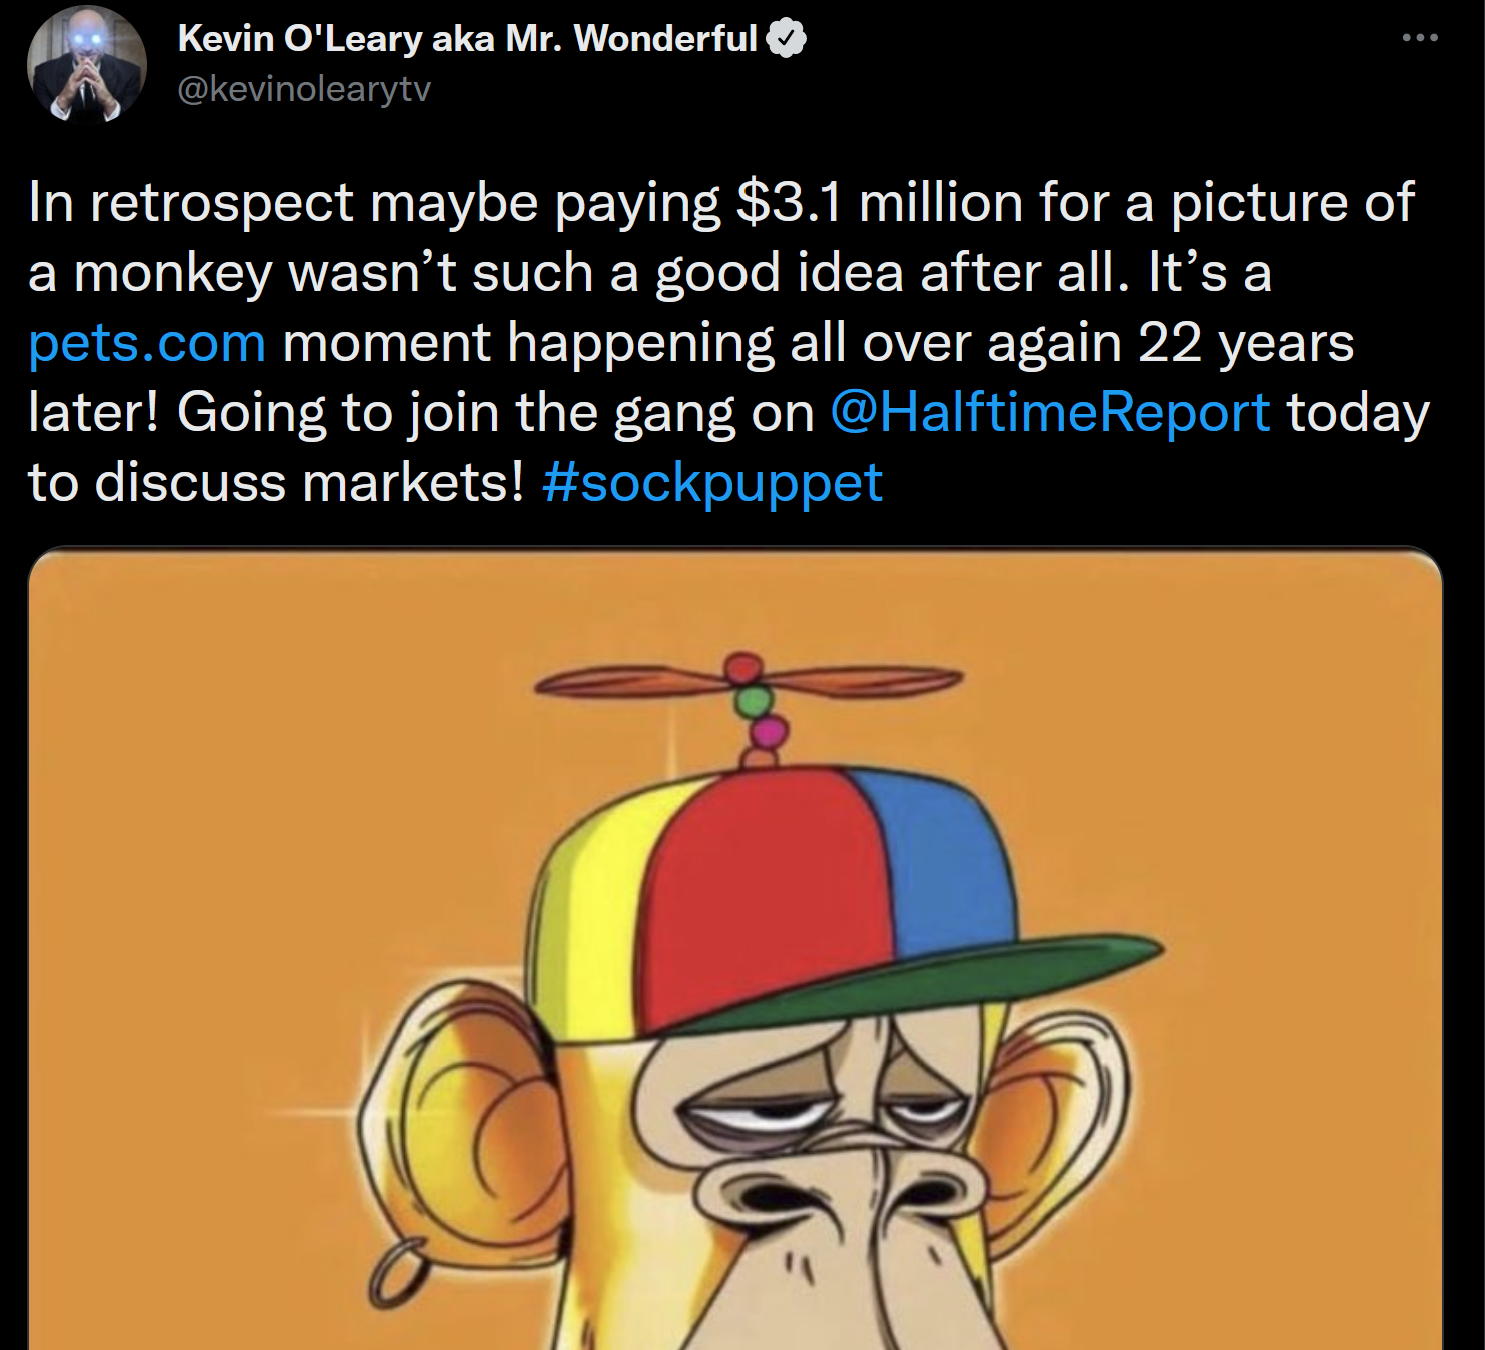
\includegraphics[width=\linewidth]{monkey}
	\caption{The \href{https://www.coingecko.com/en/nft/bored-ape-yacht-club}{bubble bursts} on Yuga Bored Apes for now.}
	\label{fig:monkey}
\end{figure*}

%Samsung for instance have announced that their TVs will support not only \href{https://news.samsung.com/us/samsung-2022-micro-led-neo-qled-lifestyle-tvs-personalization-options-ces-2022/}{display of NFTs} with artist defined settings in the metadata, but also an integrated marketplace for browsing and purchasing.\par
One of the most interesting companies is Yuga Labs, who launched the incredibly popular Bored Ape Yacht club set of 10,000 algorithmically generated NFTs. These Ethereum based NFTs were based loosely on the `Crypto Punks' model of PFP-NFT (variously profile picture project, picture for proof, and picture for profile - no definition remains uncontested for long). Yuga launched with a better commercialisation model for the holders, and a strong marketing drive into celebrity circles. They now regularly change hands for hundreds of thousands of pounds. Even this `blue chip' NFT is not without \href{https://twitter.com/coryklippsten/status/1538909505236283392}{serious criticism}: \textit{``I'd put it at 99.99\% the project is in fact a deliberate troll, intentionally replete with Nazi symbols and esoteric racist dog whistles''}\par
Yuga recently bought the artistic rights to the commercial reuse of similarly popular (and preceding) Punks set. This is interesting because they have again handed the commercial re-use rights to the owners of the individual NFTs. This raises the same \href{https://www.bloomberg.com/news/articles/2022-03-21/bored-ape-nft-spinoff-venture-gone-sour-sparks-legal-fight}{confusing problem} with attaching commercial rights to an easily stolen token as NFTs for real estate does. This has been demonstrated recently when Seth Green had a Bored Ape stolen after \href{https://www.buzzfeednews.com/article/sarahemerson/seth-green-bored-ape-stolen-tv-show}{creating an animated show around it's IP}.  \par
The community around these collections is incredibly strong, mixing developers, artists, the rich and famous, and the fortunate and early, into a cohesive community who communicate online. The developer `good will' is enormous, and it seems possible that this will lead to faster and broader innovation around the collections, and out into \href{https://twitter.com/yugalabs/status/1505014986556551172?}{metaverse applications}. The brand is strong, and the individual NFT items both benefit from, and reinforce that brand, while adding personal narratives and human interest.\par 
As a gauge of how frothy this market still is it's interesting to look at the APE token which Yuga just launched. They airdropped 10,000 of the tokens free to each of the 10,000 NFT holders. This instantly created a multi-billion dollar market cap, and a top 50 `crypto' out of thin air, based purely on their brand. It's clear that there is both brand, and a market here.\par
A recent report from "Base Layer" tries to capture the community `feature' of big brand NFTs. \href{https://baselayer.so/crypto-culture-decoded}{``Crypto culture decoded''} explains that is is these online communities which are the attraction not necessarily the art. This is a powerful `in group' argument, though speculation remains the most likely underpinning.



%\href{https://amycastor.com/2021/03/14/metakovan-the-mystery-beeple-art-buyer-and-his-nft-defi-scheme/}{Beeple scam}


\section{Objects in our metaverse}
NFTs seem to be judged crucial to metaverse applications. Meta (ex Facebook) are hanging their monetisation of their whole rebrand on taking a huge cut from NFT content creators on their platform.\par
We have a path to assets and NFTs within the layer 3 elements of our choices (RGB), but they're not yet fit for purpose. There are compromise options already available, as below.
\subsection{Liquid tokens}
We have seen that Liquid from Blockstream is a comparatively mature and battle tested sidechain framework, based upon Bitcoin. It is possible to issue tokens on Liquid, and these have their own hardware wallet available. This makes the technology a strong contender for our uses.
\subsection{Sovryn and RSK}
It's slightly unclear when RSK will support assets at this level. This needs to be revisited.
\subsubsection{Optimistic rollups}
\lipsum[50]
\subsubsection{Zero Knowledge rollups}
\lipsum[50]
\subsection{Stacks and STX}
There's another possible option is Stacks, without the network effect of Ethereum, but closer to the other design choices made so far. ``Stacks is an open-source network of decentralized apps and smart contracts built on Bitcoin.''\\ 
This novel approach saw the launch of a layer 1 blockchain token called STX, which is used in a similar way to gas in Ethereum. but claims settlement on the Bitcoin network. This is achieved through a novel bridging approach which they call Proof of Transfer (PoX).\\
Stacks users say this hybrid approach is a pragmatic solution which enables dApps, smart contracts, DeFi, NFTs etc without compromising security. In practice the speculative component of the STX tokens which underpin these operations clouds the issue somewhat. It is a potentially useful middle ground solution with a great deal of developer attention.
\subsection{Ethereum}
While it's been discounted elsewhere it's hard to ignore the network effect of Eth NFTs. If the aspiration is to attract the bulk of the `legacy' creator/consumer markets then it will be necessary to support integration of Metamask into any FOSS stack. This isn't a huge technical challenge, nor is it particularly of interest to our use cases at this stage, but it remains a possibility. The main problems remain the slow speed and high expense of the system.
\subsection{Solana}
Solana is both cheap and fast, because it's very highly centralised. It seems unlikely that it's worth this level of compromise.
\subsection{Satoshi Ordinals}
Satoshi ordinals \href{https://github.com/casey/ord}{allow tracking of Sats across transactions}, enabling NFT like assignment tracking. This is a hugely exciting development but extremely early.
\subsection{Peerswap}
It may be possible to use ``Peerswap'' to execute rebalancing and submarine swaps into and out of Liquid assets on the sidechain in a single tx. This is anunder explored area at this time.
\subsection{FROST on Bitcoin}
It \textbf{might} be possible to transfer ownership of a UTXO on the Bitcoin base chain using FROST \cite{komlo2020frost}. In this Schnorr \& Taproot based threshold signature system it's possible to \href{https://btctranscripts.com/sydney-bitcoin-meetup/2022-03-29-socratic-seminar/}{add and remove signatories} and thresholds of signing without touching the UTXO itself. In principle (though not yet in practice) this might allow transfer of UTXO ownership. 
\subsection{Spacechains}
It feels like spacechains are almost ready, so this is worth keeping an eye on. It's the `cleanest' way to issue assets using Bitcoin because there's no additional speculative chain. As briefly explained in the earlier section Bitcoin is destroyed to create a new chain which then inherits the security of Bitcoin through onward mining. This new asset or chain is able to accrue value and trade independently based purely on it's value to the buyer, not as a function of a wider speculative bubble attached to a token with multiple use cases.


\chapter{Metaverses}
\section{Toward an open metaverse}
For our purposes in this book and product design the interface between the previous chapter (NFTs) and this metaverse chapter is crucial. Punk6529 is a pseudonymous twitter account and thought leader in the ``crypto'' space. The text below encapsulates much of the reasoning that led to this book and product exploration, and is paraphrased \href{https://twitter.com/punk6529/status/1536046831045685248}{from this thread} for our purposes.\par
\textit{Bit by bit, the visualization layer of the internet will get better until it is unrecognisably better (+/- 10 years). As the visualization layer of the internet gets better, digital objects will become more useful and more important. Avatars (2D and 3D), art, schoolwork, work work, 3D virtual spaces and hundreds of other things. Not only will the objects themselves become more important, they will lead to different emergent behaviours. We see this already with avatars and mixed eponymous/pseudonymous/anonymous communities. Yes, it is the internet plumbing underneath, but just like social media changed human behaviour on the internet, metaverse type experiences will further change it. NFT Twitter + Discord + various virtual worlds is a form of early metaverse. I feel like I am entering a different world here, not just some websites. The most important question for the health of the internet/metaverse/human society in the 2030s will be decided now. And that question is: "who stores the definitive ownership records of those digital objects". There are two answers: a company's database OR a blockchain. If we end up with "a company's database" we will end up with all the web2 dysfunctions, but worse. SMTP is an open protocol that anyone can use so we don't have societal level fights on "who is allowed to use email". Short messaging online ended up becoming Twitter. So we end up having the most absurd, surreal discussions on the topic of "who is allowed to use short-messaging" being dependant on "who is the CEO of Twitter". There is no way this is the correct architecture for our progressively more digital economy.... If this is your first time around here, we are fighting for an open metaverse.''}\par
It seems that industry shares much of this opinion regarding an open metaverse. The proposal of a persistent interactive digital universe online is \textbf{so} vast that major players recognise that they will not be able to monopolise this space, though Facebook/Meta are clearly attempting to. The \href{https://metaverse-standards.org/news/press-releases/leading-standards-organizations-and-companies-unite-to-drive-open-metaverse-interoperability/}{Metaverse Standards Forum} is clearly an attempt by the other industry players to catch up and then get out ahead of Meta in this regard. It's also possible to view this as just another land grab, but through the vehicle of a standards body. Time will tell. They say:\par
\textit{``Announced today, The Metaverse Standards Forum brings together leading standards organizations and companies for industry-wide cooperation on interoperability standards needed to build the open metaverse. The Forum will explore where the lack of interoperability is holding back metaverse deployment and how the work of Standards Developing Organizations (SDOs) defining and evolving needed standards may be coordinated and accelerated. Open to any organization at no cost, the Forum will focus on pragmatic, action-based projects such as implementation prototyping, hackathons, plugfests, and open-source tooling to accelerate the testing and adoption of metaverse standards, while also developing consistent terminology and deployment guidelines.''}\par
This looks like it will be a useful project and community for the purposes outlined in this book, but the technology is young enough (in that it doesn't really exist) for multiple approaches to be trailed.
\subsection{Primitives}
The Metaverse Standard Forum highlights the following, which reads like the output from a brainstorm between academia and industry stakeholders.
\begin{itemize}
\item collaborative spatial computing
\item interactive 3D graphics 
\item augmented and virtual reality
\item photorealistic content authoring
\item geospatial systems
\item end-user content tooling
\item digital twins
\item real-time collaboration
\item physical simulation
\item online economies
\item multi-user gaming
\item new levels of scale and immersiveness. 
\end{itemize}
It's not a useless list by any means, but it lacks the kind of product focus we need for detailed exploration of value and trust transfer. \par
John Riccitiello, CEO of Unity Technologies says that metaverse is \textit{``The next generation of the internet that is (1) always real-time and (2) mostly 3D (3) mostly interactive, (4) mostly social and (5) mostly persistent''}. This is a useful (if still quite vague) framework. Expanding this slightly we will us the following primitives of what we think are important for a metaverse:
\begin{itemize}
\item Fusing of digital and real life
\item Social first
\item Real time interactive 3d graphics first
\item Persistent
\item Supports ownership
\item Open
\item Trusted / secure
\end{itemize} 
Added to this are externalities such as the shifting exceptions of younger demographics.
\begin{itemize}
\item Convergence of film and games
\item Blurring of IP boundaries
\item Blurring of narrative flow
\item User generated content
\item Mobile first experiences
\item Safeguarding, and governance
\end{itemize}
There is a \textbf{lot} of work for the creative and technical industries to do to integrate human narrative creativity this nascent metaverse, and it's not even completely clear that this is possible, or even what people want.
\section{History}
\textbf{This chapter is being rewritten now.} %[\href{https://scholar.google.com/citations?hl=en&user=jE9vLG0AAAAJ&view_op=list_works}{Rabindra+Ratan} notes to include new researchers in the lit survey].\par
The word metaverse was coined by the author Neal Stephenson in his 1992 novel Snowcrash. It started popping up soon after in \href{https://www.newscientist.com/article/mg14819994-000-how-to-build-a-metaverse/}{news articles} and research papers \cite{mclellan1993avatars}, but in the last five years it has been finding a new life within a silicon valley narrative.\par
There were clear precursors to modern social VR, such as \href{https://www.howtogeek.com/778554/remembering-vrml-the-metaverse-of-1995/}{VRML in the 1990's} which laid much of the groundwork for 3D content over networked computers.\par% The author used to create commercial 3D scenes on Silicon Graphics systems back in the late 90s.\par
It might seem that there would be a clear path from there to now, in terms of a metaverse increasingly meaning connected social virtual spaces, but this has not happened. Instead interest in metaverse as a concept waned, MMORG (described later) filled in the utility, and then recently an entirely new definition emerged. The concept of the Metaverse is extremely plastic at this time (Figure \ref{fig:muskWeb3}).\par
It's arguable that what will be expanding in this chapter is more appropriately `Cyberspace' as described by William Gibson in Neuromancer \cite{gibson2019neuromancer} \textit{``A global domain within the information environment consisting of the interdependent network of information systems infrastructures including the Internet, telecommunications networks, computer systems, and embedded processors and controllers.''}\par
The book will aim to build toward an understanding of metaverse as a useful social mixed reality, that allows low friction communication and economic activity, within groups, at a global scale. Cryptography and distributed software can assist us with globally `true' persistence of digital data, so we will look to integrate this with our social XR.  This focus on persistence, value, and trust means it's most appropriate to focus on business uses as there is more opportunity for value creation which will be important to bootstrap this technology.\par
This chapter will first attempt to frame the context for telepresence (the academic term for communicating through technology), and then explain the increasingly polarised options for metaverse. It's useful to precisely identify the primitives of the product we would like to see here, so this chapter is far more a review of academic literature in the field, culminating in a proposed framework.\par
\begin{figure}
  \centering
    
\includegraphics[width=\linewidth]{muskWeb3}
  \caption{Elon Musk agrees with this on Twitter. It's notable that Musk is now Twitters' \href{https://twitter.com/paraga/status/1511320953598357505}{biggest shareholder}, and has been vocal about Web2 censorship on the platform.}
  \label{fig:muskWeb3}
\end{figure}

\section{Business communication tools}
\subsection{Traditional telepresence}
Video-conferencing has become more popular as technology improves, and with increasing demands for real-time communication across greater distances. The full effects of video-conferencing on human communication are still being explored. Video-conferencing is presumed to be a somewhat richer form of communication than email and telephone, but not quite as informative as face-to-face communication. In this section we look at the influence of eye contact on communication and how video-conferencing mediates both verbal and non-verbal interactions. Facilitation of eye contact is a challenge that must be addressed so that video-conferencing can approach the rich interactions of face-to-face communication. This is an even bugger problem in the emerging metaverse systems, so it's important that we examine the history and trajectory.\\
Connection of multiple users is now well supported through technologies such as telephony \& webcams, with Zoom and \href{https://www.microsoft.com/en-us/Investor/earnings/FY-2021-Q1/press-release-webcast}{Mircosoft Teams} alone supporting hundreds of millions of chats a day. This is a 20x increase on market leader Skype's 2013 figure of \href{https://www.microsoft.com/en-us/Investor/earnings/FY-2013-Q1/press-release-webcast}{280 million} connections per month. Such technologies extend traditional telephony to provide important multi sensory cues (non-verbal communication \cite{Argyle1976, Wolff2008}).  However, these technologies demonstrate shortfalls compared to a live face-to-face meeting, which is generally agreed to be optimal for human-human interaction \cite{Wolff2008}.\\
In an experiment at CTrip, Bloom et al describe how home working led to a 13\% performance increase, of which about 9\% was from working more minutes per shift (fewer breaks and sick-days) and 4\% from more calls per minute (attributed to a quieter working environment) \cite{Bloom2015}. Home workers also reported improved work satisfaction and experienced less turnover, but their promotion rate conditional on performance fell. Due to the success of the experiment, CTrip rolled-out the option to WFH to the whole firm and allowed the experimental employees to re-select between the home or office. Interestingly, over half of them switched, which led to the gains from WFH almost doubling to 22\%. This highlights the benefits of learning and selection effects when adopting modern management practices like WFH.\\
Enterprise collaboration systems provide rich document management, sharing, and collaboration functionality across an organisation. The enterprise ECS system may integrate collaborative video \cite{prakash2020characteristic}. This is for instance the case with Microsoft Teams / Sharepoint. This integration of ECS should be considered when thinking about social VR systems which wish to support business, value, and trust.\\
\subsubsection{Pandemic drives adoption}
The ongoing global COVID-19 pandemic is changing how people work, toward a new global 'normal'. Some ways of working are overdue transformation, and will be naturally disrupted. In the UK at least it seems that there may be `real appetite' to shift away from old practises \cite{skychange}. This upheaval will inevitably present both challenges and opportunities.\\
Highly technical workforces, especially, can \href{https://globalworkplaceanalytics.com/telecommuting-statistics}{operate from anywhere}. Bloom at al found that the 10\% of home workers surveyed in 2013 enjoyed increased performance and satisfaction, and reduced staff turnover \cite{Bloom2015}. Little seems to have changed since then, until the recent pandemic forced the hand of global business. If only a small percentage of companies allow the option of remote working, then they gain a structural advantage, enjoying benefits of reduced travel, lower workplace infection risk across all disease, and global agility for the personnel. Building and estate costs will certainly be reduced. More diversity may be possible. Issues such as sexual harassment and bullying may be reduced.  With reduced overheads product quality may increase. If customers are happier with their services, then over time this `push' may mean an enormous shift away from centralised working practises toward distributed working. \\
Technologies which can support this working style are (surprisingly) still in their infancy. The rush to `Zoom', a previously relatively unknown and insecure \cite{aiken2020zooming} web meeting product, shows how naive businesses were in this space. \\
While the research community and business are learning how to adapt working practises to web based telepresence \cite{oeppen2020human}, there remains little technology support for ad-hoc serendipitous meetings between small groups. It's possible that Metaverse applications can help to fill this gap, by gamification of social spaces.\\


\subsection{Extra verbal content}
Additional to the semantic content of verbal communication there is a rich layer of meaning in pauses, gaps, interruptions, and overlaps \cite{Heldner2010} which help to mediate who is speaking and who is listening in multi-party conversation. This mediation of turn passing, to facilitate flow, is by no means a given and is highly dependent on context and other factors \cite{Kleinke1986a}. This stuff is a huge challenge in conventional telepresence, and even more so in third person metaverse applications. \\ 
This extra-verbal content \cite{ting2012understanding} extends into physical cues, so-called `nonverbal' cues, and there are utterances which link the verbal and non-verbal \cite{Otsuka2005}. This will be discussed later, but to an extent, it is impossible to discuss verbal communication without regard to the implicit support which exists around the words themselves. \\
In the context of all technology-mediated conversation the extra-verbal is easily compromised if technology used to support communication over a distance does not convey the information, or conveys it badly. This can introduce additional complexity \cite{Otsuka2005}. These support structures are pretty much lacking in metaverse XR systems. The goal then here perhaps is to examine the state of the art, and remove as many of the known barriers as possible. Such a process might better support trust, which might better support the kind of economic and activity we seek to engineer.\\
\subsection{Audio}
Even in simple voice telephony, system latency, the inherent delays added by the communication technology, can allow slips or a complete breakdown of 'flow' \cite{Katagiri2007}.\\
It seems that transmission of verbal / audio is the most critical element for interpersonal communication since the most essential meaning is encoded semantically. There is a debate about ratios of how much information is conveyed through the various human channels \cite{loomis2012sensory}, but it is reasonable to infer from its ubiquity that support for audio is essential for meaningful communication over a distance. We have seen that it must be timely, to prevent a breakdown of framing, and preferably have sufficient fidelity to convey sub-vocal utterances. For business users of metaverse tools this implies that much better microphones are important, and spatial audio cues within the environment, keyed to the head position. \\
\subsection{Nonverbal}
We have already seen that verbal exchanges take place in a wider context of sub vocal and physical cues. In addition, the spatial relationship between the parties, their focus of attention, their gestures and actions, and the wider context of their environment all play a part in communication \cite{Goodwin2000a}. These are summarised well by Gillies and Slater \cite{Gillies2005} in their paper on virtual agents. In support of this an immersive virtual gathering should have as wide a field of view as possible. This is principally are hardware constraint, though an over wide FOV can be compressed into a smaller hardware display with ``some'' user discomfort.\\
\subsubsection{Gaze}
Of particular importance is judgement of eye gaze which is fast, accurate and automatic, operating at multiple levels of cognition through multiple cues \cite{Argyle,argyle1976gaze,Argyle1965,Argyle1976,Argyle1969, Kendon1967,Monk2002}.\\
Gaze in particular aids with smooth turn passing \cite{Hedge1978} \cite{Novick1996} and lack of support for eye gaze has been found to decrease the efficiency of turn passing by 25\% \cite{Vertegaal00effectsof}.\\
There are clear patterns to eye gaze in groups, with the person talking, or being talked to, probably also being looked at \cite{Vertegaal2001} \cite{Langton2000}. To facilitate this groups will tend to position themselves to maximally enable observation of the gaze of the other parties \cite{Kendon1967}. This intersects with proxemics which will be discussed shortly.  In general people look most when they are listening, with short glances of 3-10 seconds \cite{Argyle1965}. 
Colburn et al. suggest that gaze direction and the perception of the gaze of others directly impacts social cognition \cite{Colburn2000a} and this has been supported in a follow up study \cite{Macrae2002}.\\
The importance of gaze is clearly so significant in evolutionary terms that human acuity for eye direction is considered high at ~30 sec arc \cite{Symons2004} with straight binocular gaze judged more accurately than straight monocular gaze \cite{Kluttz2009}, when using stereo vision. \\
Regarding the judgement of the gaze of others Symons et al. suggesting that ``people are remarkably sensitive to shifts in a person's eye gaze'' in triadic conversation \cite{Symons2004}. Wilson et al. found that subjects can ``discriminate gaze focused on adjacent faces up to [3.5m]'' \cite{Wilson2000}\\
Schrammel et al. investigated to what extent embodied agents can elicit the same responses in eye gaze detection \cite{Schrammel2007}.\\
This perception of the gaze of others operates at a low level and is automatic. Langton et al. cite research stating that the gaze of others is ``able to trigger reflexive shifts of an observer's visual attention'' and further discuss the deep biological underpinnings of gaze processing \cite{doi:10.1080/713755908}. \\          
When discussing technology-mediated systems Vertegaal \& Ding suggested that understanding the effects of gaze on triadic conversation is ``crucial for the design of teleconferencing systems and collaborative virtual environments'' \cite{Vertegaal2002}, and further found correlation between the amount of gaze, and amount of speech. Vertegaal \& Slagter suggest that ``gaze function(s) as an indicator of conversational attention in multiparty conversations'' \cite{Vertegaal2001}. \\        
Vertegaal et al. found that task performance was 46\% better when gaze was synchronised in their telepresence scenario. As they point out, gaze synchronisation (temporal and spatial) is `commendable' in all such group situations, but the precise utility will depend upon the task \cite{Vertegaal2002}.\\
There has been some success in the automatic detection of the focus of attention of participants in multi party meetings \cite{Stiefelhagen2001, Stiefelhagen2002}.  More recently, advanced eye tracking technologies allow the recording and replaying of accurate eye gaze information \cite{Steptoe2009} alongside information about pupil dilation toward determination of honesty and social presence \cite{Steptoe2010a}.\\               
In summary, gaze awareness does not just mediate verbal communication but rather is a complex channel of communication in its own right. Importantly, gaze has a controlling impact on those who are involved in the communication at any one time, including and excluding even beyond the current participants. It seems of importance for our metaverse use case that gaze be possible, if not necessarily demanded. \\
\subsubsection{Mutual Gaze}
Aygyle and Cook established a great deal of science around gaze and mutual gaze, with their seminal book of the same title \cite{argyle1976gaze}, additionally detailing confounding factors around limitations and inaccuracies in observance of gaze and how this varies with distance \cite{Argyle1969} \cite{Argyle} \cite{Cook1977}.\\
Mutual gaze is considered to be the most sophisticated form of gaze awareness with significant impact on dyadic conversation especially \cite{Cook1977, Kleinke1986a, Fagel2010}. The effects seem more profound than just helping to mediate flow and attention, with mutual eye gaze aiding in memory recall and the formation of impressions \cite{Bohannon2013}.\\
While reconnection of mutual eye gaze through a technology boundary does not seem completely necessary it is certainly important, with impact on subtle elements of one to one communication, and therefore discrimination of eye gaze direction should be bi-directional if possible, and if possible have sufficient accuracy to judge direct eye contact. In their review Bohannon et al. said that the issue of rejoining eye contact must be addressed in order to fully realise the richness of simulating face to face encounters \cite{Bohannon2013}.\\
Mutual gaze is a challenging affordance as bi-directional connection of gaze is not a trivial problem. All users would need to be immersed and using eye trackers properly. There is no technical impediment here, but rather one of adoption curves.
\subsubsection{Head Orientation}
Orientation of the head (judged by the breaking of bilateral symmetry and alightment of nose) is a key factor when judging attention. Perception of head orientation can be judged to within a couple of degrees \cite{Wilson2000}.\\
It has been established that head gaze can be detected all the way out to the extremis of peripheral vision, with accurate eye gaze assessment only achievable in central vision \cite{Loomis2008}. Features of illumination can alter the apparent orientation of the head \cite{Troje1998}; as usual the wider context is in play.\\
Head motion over head orientation is a more nuanced proposition and can be considered a micro gesture \cite{Boker2011}.\\
Regarding video mediated teleconferencing;  Vertegaal  et al. \cite{Vertegaal00effectsof} note that  the ``larger the distance of head to screen, or the smaller the projected images, the more head movement of users is tolerable without impairing the conveyance of gaze at the eyes''. While users of video conferencing equipment tend to position themselves correctly in front of the camera, movement speed of the head within the frame during use is typically in the region 2-3 meters per second. Framerate of the camera should support this \cite{Bocker1996}.\\
                    It is possible that 3D displays are better suited to perception of head gaze since it is suggested that they are more suitable for ``shape understanding tasks'' \cite{john2001use}\\
                    Bailenson, Baell, and Blascovich found that giving avatars rendered head movements in a shared virtual environment decreased the amount of talking, possibly as the extra channel of head gaze was opened up. They also reported that subjectively, communication was enhanced \cite{Bailenson2002}. \\
                    Clearly head orientation is an important indicator of the direction of attention of members of a group and can be discerned even in peripheral vision. This allows the focus of several parties to be followed simultaneously and is an important affordance to replicate on any multi-party communication system. Head gaze comes for free in immersive headset participation within a metaverse, but how to handle users who do not have a headset?\\
\subsubsection{Combined Head and Eye Gaze}
Rienks et al. found that head orientation alone does not provide a reliable cue for identification of the speaker in a multiparty setting \cite{Rienks2010}. Stiefelhagen \& Zhu found ``that head orientation contributes 68.9\% to the overall gaze direction on average'' \cite{Stiefelhagen:2002:HOG:506443.506634}, though head and eye gaze seem to be judged interdependently \cite{Kluttz2009}. Langton noted that head and eye gaze are ``mutually influential in the analysis of social attention'' \cite{Langton2000a}, and it is clear that transmission of `head gaze' by any mediating system enhances rather than replaces timely detection of subtle cues. Combined head and eye gaze give the best of both worlds and extend the lateral field of view in which attention can be reliably conveyed to others. This implied both head AND eye tracking for participants in the metaverse. There are edge cases here where eye tracking might be present without head tracking, and they should be identified in the system.\\

\subsection{Presence, Co-presence, and Social Presence}
Presence is a heavily cited historic indicator of engagement in virtual reality, though the precise meaning has been interpreted differently by different specialisms \cite{Beck2011, Schuemie2001}. It is generally agreed to be the 'sense of being' in a virtual environment \cite{Slater1999}. Slater extends this to include the ``extent to which the VE becomes dominant". \\
Beck et al. reviewed 108 articles and synthesised an ontology of presence \cite{Beck2011} which at its simplest is as follows:
            \begin{enumerate}
				\item Sentient presence
                    \begin{enumerate}
                     \item Physical interaction
                      \item Mental interaction
                    \end{enumerate}
                   \item Non-sentient
                   \begin{enumerate}
                       \item Physical immersion
                       \item Mental immersion = psychological state
                     \end{enumerate}
            \end{enumerate}
When presence is applied to interaction it may be split into Telepresence, and Co/Social presence  \cite{heeter1992being, Biocca1997}.  Co-presence and/or social presence is the sense of ``being there with another", and describes the automatic responses to complex social cues \cite{doi:10.1080/01449299508914633, fulk1987social, haythornthwaite1995work}.    Social presence (and co-presence) refers in this research context to social presence which is mediated by technology (even extending to text based chat \cite{Gunawardena1997}), and has its foundations in psychological mechanisms which engender mutualism in the `real'. This is analysed in depth by Nowak \cite{Nowak2001}. An examination of telepresence, co-presence and social presence necessarily revisits some of the knowledge already elaborated.\\
        The boundaries between the three are blurred in research with conflicting results presented \cite{Bulu2012}. Biocca et al. attempted to enumerate the different levels and interpretations surrounding these vague words \cite{Biocca2003}, and to distill them into a more robust theory which better lends itself to measurement. They suggest a solid understanding of the surrounding psychological requirements which need support in a mediated setting, and then a scope that is detailed and limited to the mediated situation.\\
 Since `social presence' has been subject to varied definitions \cite{Biocca2003} it is useful here to consider a single definition from the literature which defines it as ``the ability of participants in the community of inquiry to project their personal characteristics into the community, thereby presenting themselves to the other participants as real people.'' \cite{Garrison1999, Beck2011}. Similarly to specifically define co-presence for this research it is taken to be the degree to which participants in a virtual environment are ``accesible, available, and subject to one another" \cite{Biocca2003}. \\
            Social presence has received much attention and there are established questionnaires used in the field for measurement of the levels of perceived social presence yet the definitions here also remain broad, with some confusion about what is being measured \cite{Biocca2003a}.\\            
 Telepresence meanwhile is interaction with a different (usually remote) environment which may or may not be virtual, and may or may not contain a separate social/co-presence component. \\ 
       Even in simple videoconferencing Bondareva and Bouwhuis stated (as part of an experimental design) that the following determinants are important to create social presence \cite{Bondareva2004, jouppi2002mutually}. 
            \begin{enumerate}
            \item    Direct eye contact is preserved
            \item    Wide visual field
            \item    Both remote participants appear life size
            \item    Possibility for participants to see the upper body of the interlocutor
            \item    High quality image and correct colour reproduction
            \item    Audio with high S/N ratio
            \item    Directional sound field
            \item    Minimization of the video and audio signal asynchrony
            \item    Availability of a shared working space.
            \end{enumerate}
			
			     
            Bondareva et al. went on to describe a person to person telepresence system with a semi silvered mirror to reconnect eye gaze, which they claimed increased social presence indicators. Interestingly they chose a checklist of interpersonal interactions which they used against recordings of conversations through the system \cite{Bondareva2004}.  \\
            The idea of social presence as an indicator of the efficacy of the system suggests the use of social presence questionnaires in the evaluation of the system \cite{Biocca2003}.  Subjective questionnaires are however troublesome in measuring effectiveness of virtual agents and embodiments, with even nonsensical questions producing seemingly valid results \cite{Slater2004}. Usoh et al. found that 'the real' produced only marginally higher presence results than the virtual \cite{Usoh2000a}.\\
            Nowak states that ``A satisfactory level of co-presence with another mind can be achieved with conscious awareness that the interaction is mediated" and asserts that while the mediation may influence the degree of co-presence it is not a prohibiting factor \cite{Nowak2001}.\\ 
            Baren and IJsselsteijn \cite{Baren, Harms2004} list 20 useful presence questionnaires in 2004 of which ``Networked Minds" seemed most appropriate for the research.
            Hauber et al. employed the ``Networked Minds" Social Presence questionnaire experimentally and found that while the measure could successfully discriminate between unmediated and mediated triadic conversation, it could not find a difference between 2D and 3D mediated interfaces \cite{Hauber2005, Gunawardena1997}.
            \\In summary, social presence and co-presence are important historic measures of the efficacy of a communication system. Use of the term in literature peaked between 1999 and 2006 according to Google's ngram viewer and has been slowly falling off since. The questionnaire methodology has been challenged in recent research and while more objective measurement may be appropriate, the networked minds questions seem to be able to differentiate real from virtual interactions \cite{Harms2004}.
 
\subsection{Mutual Gaze in Telepresence}
          We have seen that transmission of attention can broadly impact communication in subtle ways, impacting empathy, trust, cognition, and co-working patterns. Mutual gaze (looking into one another's eyes), is currently the high water mark for technology-mediated conversation.\\
          Many attempts have been made to re-unite mutual eye gaze when using tele-conferencing systems. In their 2015 review of approaches Regenbrecht and Langlotz found that none of the methods they examined were completely ideal \cite{Regenbrecht2015}. They found most promise in 2D and 3D interpolation techniques, which will be discussed in detail later, but they opined that such systems were very much ongoing research and lacked sufficient optimisation.\\
          A popular approach uses the so called 'Peppers Ghost' phenomenon \cite{steinmeyer2013science}, where a semi silvered mirror presents an image to the eye of the observer, but allows a camera to view through from behind the angled mirror surface. The earliest example of this is Rosental's two way television system in 1947 \cite{rosenthal1947two}, though Buxton et al. `Reciprocal Video Tunnel' from 1992 is more often cited \cite{buxton1992telepresence}. This optical characteristic isn't supported by RPT technology, and besides requires careful control of light levels either side of the semi-silvered surface.\\  
The early GAZE-2 system (which makes use of Pepper's ghost) is novel in that it uses an eye tracker to select the correct camera from several trained on the remote user. This ensures that the correct returned gaze (within the ability of the system) is returned to the correct user on the other end of the network \cite{Vertegaal2003}.
Mutual gaze capability is later highlighted as an affordance supported or unsupported by key research and commercial systems.                           

\subsubsection{Tabletop and Shared Task}
In early telepresence research Buxton and William argued through examples that ``effective telepresence depends on quality sharing of both person and task space \cite{Buxton1992a}.\\
In their triadic shared visual workspace Tang et al. found difficulty in reading shared text using a `round the table' configuration, a marked preference for working collaboratively on the same side of the table. They also found additional confusion as to the identity of remote participants \cite{Tang2010}.
Tse et al. found that pairs can work well over a shared digital tabletop, successfully overcoming a single user interface to interleave tasks \cite{Tse2007}.\\
Tang et al. demonstrate that collaborators engage and disengage around a group activity through several distinct, recognizable mechanisms with unique characteristics \cite{Tang2006}. They state that tabletop interfaces should offer a variety of tools to facilitate this fluidity.\\
Camblend is a shared workspace which is hybrid physical and digital and which maintains some spatial cues between locations \cite{Norris2013a, Norris2012}. Participants successfully resolved such co-orientation within the system.\\
The t-room system implemented by Luff et al. surrounds co-located participants standing at a shared digital table with life sized body and head video representations of remote collaborators \cite{Luff2011} but found that there were incongruities in the spatial and temporal matching between the collaborators which broke the flow of conversation.
Tuddenham et al. found that co-located collaborators naturally devolved 'territory' of working when sharing a task space, and that this did not happen the same way with a tele-present collaborator \cite{tuddenham2009territorial}. Instead remote collaboration adapted to use a patchwork of ownership of a shared task. It seems obvious to say that task ownership is a function of working space, but it is interesting that the research found no measurable difference in performance when the patchwork coping strategy was employed.\\
The nature of a shared collaborative task and/or interface directly impacts the style of interaction between collaborators. This will have a bearing on the choice of task for experimentation \cite{Jamil2011, Jetter2011a}.

            \subsubsection{Spatially Faithful Group}
                Hauber et al. combined videoconferencing, tabletop, and social presence analysis and tested the addition of 3D. They found a nuanced response when comparing 2D and 3D approaches to spatiality: 3D showed improved presence over 2D (chiefly through gaze support), while 2D demonstrated improved task performance because of task focus \cite{Hauber2006}.\\
                I3DVC reconstructs participants from multiple cameras and places them isotropically (spatially faithful) \cite{Kauff2002, Kauff2002a}. The system uses a large projection screen, a custom table, and carefully defined seating positions. They discussed an ``extended perception space" which used identical equipment in the remote spaces in a tightly coupled collaborative `booth'. It employed head tracking and multi camera reconstruction alongside large screens built into the booth. This system exemplified the physical restrictions which are required to limit the problems of looking into another space through the screen. Towles et al. \cite{Fuchs:2002ww} demonstrated a similar system over a wide area network but achieved only limited resolution and frame rate with the technology of the day. \\ University of Southern California used a technically demanding set-up with 3D face scanning and an autostereoscopic 3D display to generate multiple `face tracked' viewpoints \cite{jones2009headspin}. This had the disadvantage of displaying a disembodied head.\\                
MAJIC is an early comparable system to support small groups with life size spatially correct video, but without multiple viewpoints onto the remote collaborators it was a one to 'some' system rather than 'some' to one. Additionally users were rooted to defined locations \cite{Ichikawa1995, Okada:1994et}.\\
\textbf{Multiview}

In order to reconnect directional cues of all kinds it is necessary for each party in the group to have a spatially correct view of the remote user which is particular for them. This requires a multi-view display, which has applications beyond telepresence but are used extensively in research which attempts to address these issues.\\
Nguyen and Canny demonstrated the `Multiview' system \cite{Nguyen2005}. Multiview is a spatially segmented system, that is, it presents different views to people standing in different locations simultaneously. They found similar task performance in trust tasks to face to face meetings, while a similar approach without spatial segmentation was seen to negatively impact performance.\\
In addition to spatial segmentation of viewpoints it is possible to isolate viewpoints in the time domain. Different tracked users can be presented with their individual view of a virtual scene for a few milliseconds per eye, before another viewpoint is shown to another user. Up to six such viewpoints are supported in the c1x6 system \cite{Kulik2011}
Similarly MM+Space offered 4 Degree-Of-Freedom Kinetic Display to recreate Multiparty Conversation Spaces \cite{Otsuka2013}
            \subsubsection{Robots, Shader Lamp, and Hybrid}
                Virtuality human representation extends beyond simple displays into robotic embodiments (which need not be humanoid \cite{Marti2005}), shape mapped projection dubbed ``shader lamps", and hybridisations of the two.\\ 
				\textbf{Uncanniness}
				
When employing simulation representations of humans it may be the case that there is an element of weirdness to some of these systems, especially those that currently represent a head without a body. Mori has demonstrated The Uncanny Valley \cite{Mori1970} effect in which imperfect representations of humans elicit revulsion in certain observers. This provides a toolkit for inspecting potentially `weird' representations, especially if they are `eerie' and is testable through Mori's GODSPEED questionnaire. \\
                    With an improved analysis of the shape of the likeability curve estimated later showing a more nuanced response from respondents where anthropomorphism of characters demonstrated increased likeability even against a human baseline \cite{Bartneck2007, Bartneck2009a}.\\
                    A mismatch in the human realism of face and voice also produces an Uncanny Valley response \cite{Mitchell2011}.\\
                    However, there is a possibility that Mori's hypothesis may be too simplistic for practical everyday use in CG and robotics research since anthropomorphism can be ascribed to many and interdependent features such as movement and content of interaction \cite{Bartneck2009}.\\
                    Bartneck et al. also performed tests which suggest that the original Uncanny Valley assertions may be incorrect, and that it may be inappropriate to map human responses to human simulacrum to such a simplistic scale. They suggest that the measure has been a convenient `escape route' for researchers \cite{Bartneck2009}. Their suggestion that the measure should not hold back the development of more realistic robots holds less bearing for the main thrust of this telepresence research which seeks to capture issues with imperfect video representation rather than test the validity of an approximation.\\
                    Interestingly Ho et al. performed tests on a variety of facial representations using images. This is far closer to the core investigation. They found that facial performance is a `double edged sword' with realism being important to robotic representations, but there also being a significant Uncanny Valley effect around `eerie, creepy, and strange' which can be avoided by good design \cite{Ho2008}.\\
                    More humanlike representations exhibiting higher realism produce more positive social interactions when subjective measures are used \cite{Yee2007a} but not when objective measures are used. This suggests that questionnaires may be more important when assessing potential uncanniness.\\
                    Ho et al. also identified problems with the original GODSPEED indices used to measure Uncanny Valley effects. They proposed a new set of measures which they found to be generally valid \cite{Ho:2010:RUV:1853385.1853509}, though they admit they were only tested with a single set of stimuli.\\
                    A far more objective method would be to measure user responses to humans, robots, and representations with functional near-infrared spectroscopy and while this has been attempted it is early exploratory research \cite{Strait2014}, an emotional response to `eerie' was discovered.\\
\textbf{Embodiment through robots}

                    Robots which carry a videoconference style screen showing a head can add mobility and this extends the available cues \cite{Adalgeirsson2010, Lee2011b, Tsui2011, Paulos1998, Kristoffersson2013}. Interestingly Desai and Uhlik maintain that the overriding modality should be high quality audio \cite{Desai2011}.\\
                    Tsui et al. asked 96 participants to rate how personal and interactive they found interfaces to be. Interestingly they rated videoconferencing as both more personal and more interactive than telepresence robots, suggesting that there is a problem with the overall representation or embodiment \cite{Tsui2012}.\\
                    Kristoffersson et al. applied the Networked Minds questionnaire to judge presence of a telepresence robot for participants with little or no experience of videoconferencing. Their results were encouraging, though they identified that the acuity of the audio channel needing improvement \cite{Kristoffersson2011}.\\
                    There are a very few lifelike robots which can be used for telepresence, and even these are judged to be uncanny \cite{Sakamoto2007}. This is only an issue for a human likeness since anthropomorphic proxies such as robots and toys perform well \cite{Mori1970}.\\
 \textbf{Physical \& Hybrid embodiment}
 
                    Embodiment through hybridisation of real-time video and physical animatronic mannequins has been investigated as a way to bring the remote person into the space in a more convincing way \cite{Lincoln2009, Lincoln:2010it, Raskar2001a}. \ These include telepresence robots \cite{Lee2011b, Sakamoto2007, Tsui2011}, head in a jar implementations such as SphereAvatar \cite{Oyekoya2012, pan2014comparing, Pan2012a} and BiReality \cite{Jouppi2004}, \ UCL's Gaze Preserving Situated Multi-View Telepresence System \cite{Pan2014a}, or screen on a stick style representations \cite{Kristoffersson2013}.\\  
                    Nagendran et al. present a 3D continuum of these systems into which they suggest all such systems can be rated from artificial to real on the three axes, shape, intelligence, and appearance \cite{Nagendran}.\\
                    Itoh et al. describe a 'face robot' to convey captured human emotion over a distance. It uses an `average face' and actuators to manipulate feature points \cite{Itoh2005}. It seems that this is an outlier method for communication of facial affect but demonstrates that there are many development paths to a more tangible human display.\\ 
\textbf{Shader lamps}

Projection mapping is a computational augmented projection technique where consideration of the relative positions and angles of complex surfaces allows the projection from single or multiple sources to augment the physical shapes onto which they appear. It was first considered by the Disney corporation in 1969 \cite{projectionmappingweb2013} and was given prominence by Raskar and Fuchs with ``office of the future" \cite{Raskar1998} and later by Raskar and other researchers \cite{Low2001, Raskar2001a}. It has since gained considerable commercial popularity in live entertainment \cite{googleStatsProjectionMapping}.\\
                    Shader lamps \cite{Raskar2001a} is the more formal academic designation for projection mapping. It is possible to use the technique alongside reconstruction to project onto a white facial mannequin. Researchers have attempted to use the technology for remote patient diagnostic, projecting onto styrofoam heads  \cite{Rivera-Gutierrez2012}.\\          
                    Lincoln et al. employed animatronic avatars which they projected with shader lamps. This combination recreated facial expression and head movement though they were limited in speed and range of control of the remote head \cite{Lincoln:2010it}.\\
                    While shader lamps are an important and useful technology, there are limitations imposed by its use. In particular if a realtime video feed or reconstruction of a subject is used then that scanned subject must either remain still enough to be correctly mapped onto geometry on the remote side (useful for some virtual patients for instance \cite{Benjamin2012}, or else there must be a computational adjustment made for their changing position to make them appear static, or the projection surface must move to match their movement as in Lincoln et al. .
 
        \subsubsection{Immersive Collaborative Virtual Environments}
Simple online virtual environments with an external viewpoint and many avatars interacting online generated much hype in the early days as a potential means to support group meetings, even back as far as the VRML standard \cite{Ferscha1999}. SecondLife in particular generated significant interest. Erickson et al. went so far as to say that a virtual conference hosted in SecondLife was 'fairly successful' \cite{Erickson2011}. For whatever reason however these systems have fallen out of favour with the public and research communities. It might be that the external viewpoint perspective, or the clunky internal viewpoint are a barrier to communication. \\
In contrast 'immersive' collaborative virtual environments place the user physically into the virtual scene. These systems are less scalable than online virtual communities which can take better advantage of distributed resources \cite{Grimstead2005a, Benford1998}. Goebbels et al. designed a taxonomy for what they termed simply CVE's. In their design they provide an excellent high level description of the ICVE as spaces which provide ``distributed collaborative teams with a virtual space where they could meet as if face-to-face, co-exist and collaborate while sharing and manipulating virtual data", crucially designed in a way to 'disburden' the users' senses \cite{Goebbels2003} and reduce fragmentation of the shared perceptual environment \cite{Roberts2005}. The ability to collaborate in such systems extends even to closely coupled physical tasks \cite{Roberts2012}.\\
There are various technology systems which demonstrate heightened immersion and presence in a virtual environment while allowing interaction between parties who may or may not be physically co-located \cite{Murray2009a}. Attempts at bringing people together in VR extend back to the early days of the technology and systems such as DIVE \cite{Benford:1995hh}. \\
                        Bailenson et al. noted that while increased realism of such avatars increases co-presence it decreases self disclosure \cite{Bailenson2006}. Such systems seem to compromise social interaction even as the realism increases. Avatar representations increased in fidelity and eventually it became possible to share avatar representations of participants wearing body tracking \cite{Schreer2005} and eye tracking equipment \cite{Garau2001, Garau2003}. This enabled tracked, viewpoint independent interaction with reconnection of eye gaze cues within VR in a spatially faithful way \cite{Roberts2003, Murray2007, Steptoe2008, Steptoe2009, Steptoe2010b}.\\
       It is also possible (at least in research implementations) to fully reconstruct people as 3D models, and connect more than two users together utilising life-size multi-view video \cite{Roberts2015, Grau2007, Divorra2010, Gross2003, Beck2013}. These 3D video representations of users can share a virtual space in which spatial and directional information are maintained in a natural way \cite{Roberts2015, Wolff2008}. \\
       Fairchild et al. have developed a system for ICVE and desktop based on earlier work by Duckworth et al. \cite{Duckworth:2012tx}, adapted for use in the Telethrone system \cite{Fairchild2016}.
            \textbf{Eye tracking in ICVE}
                More recently, advanced eye tracking technologies allow the recording and replaying of accurate eye gaze information\cite{Ciger2004a, Steptoe2009, Steptoe2008} alongside information about pupil dilation toward determination of honesty and social presence \cite{Steptoe2010a}.
            Heldal found that collaborative tasks manifested fewer disturbances due to ``misunderstandings of reference or action" when using more immersive systems \cite{Heldal2005}.
        \subsubsection{Situated Displays}
            Between the complexity of ICVEs and the more ubiquitous screen based VC technology there now exist so-called situated displays.\\
    Conversation does not exist in isolation, but rather in the context of semiotic resources. Participants make constant reference to the surrounding assets through mutual orientation, gesture, and diverse cues \cite{Goodwin2000a}.
            So called situated displays seek to embed the represented participant within the spatial and contextual framework of the conversation such that the referential cues are better supported. This has many implications, but chief amongst these is support for a spatially faithful conversational environment supportive of gaze \cite{Pan2014a, Oyekoya2012, Pan2012a, Zhang2013a}.\\
                    Such displays place a representation of the remote user into a space, theoretically allowing all participants to physically interact with the `contextual configurations' around them \cite{Goodwin2000a}. This is a relatively new field of research.  These could include the aforementioned telepresence robots \cite{Lee2011b, Sakamoto2007, Tsui2011}, head in a jar implementations such as SphereAvatar \cite{Oyekoya2012, pan2014comparing, Pan2012a},  and Gaze Preserving Situated Multi-View Telepresence System \cite{Pan2014a}.   Sphereavatar \cite{Oyekoya2012} demonstrates that there are problems with accurate mapping, distortion, and projection, and movement of the captured actors outside of very tight bounds.\\
                     Telehuman brings the whole body of a standing remote user into a space via a cylindrical display with a single tracked observer viewpoint \cite{Kim2012}.\\
            \subsubsection{Retro-reflective Projective Technology (RPT)}
Retro-reflective materials such as Chromatte(tm) cloth reflect light back along the angle of incidence. An everyday application of such material is high visibility jackets.\\
Inami et al. described the first use of RPT in 2000 with their visuo-haptic display \cite{inami2000visuo}. This system used head mounted projectors to augment RPT shapes in the real world. Krum et al. describe the REFLCT system \cite{Krum2012} which uses large retro-reflective surfaces to ``provide[s] users with a personal, perspective correct view of virtual elements that can be used to present social interactions with virtual humans''. They use helmet mounted projectors and describe a military training application in a large volume which allows faithful transmission of attention and gestures from the virtual to the real. They also briefly describe augmenting a facial mannequin by projecting onto RPT adhered to the surface. They point out that the optical characteristics of the material maintain polarisation and so could support passive stereoscopy.\\
Tachi describes an augmented reality system where a helmet mounted projector  places an image of a remote human onto a robot. This is a system they describe as Teleexistance RPT \cite{Tachi2003, Tachi2004}. This system demonstrates a single user, wearing a head mounted projector, viewing only a head which is captured from a single viewpoint. It is however enabled for motion by means of robotics under the Chromatte cloth like the hybrid robotic systems described earlier.\\
Hua et al. demonstrated elements of 'SCAPE', a tracked head mounted projection system surrounded by RPT cloth which could surround multiple physical users in a shared immersive experience \cite{Hua2004}. Hypothetically this system could be extended to include what they term 'passive remote users' projected into the views of the co-located and immersed users. The set-up however is quite complex, and involves wearing headgear, so is again less suitable for informal meetings.\\
Surman et al. discuss a potential development of their retroreflection based auto-stereoscopic display (which head tracks a single user to present a depth enabled stereo pair). They suggest that multiple users could address a large screen, but think that their stereopsis would break down and the system would be extremely challenging \cite{JSID:JSID295}.\\
Although less pertinent to this research there are other interesting deployments using RPT. Darken et al. and later Hahn in his PhD thesis in the same group describe a novel system which mounts a chromakey LED light ring and camera on a HMD \cite{Darken2003}. The camera takes in a mocked up physical cockpit and windows which are made of Chromatte cloth. This video image is very easy to segment to replace the green-screen windows with a simulated external view. The pilot trainee sees their own hands and the cockpit instrument panels (albeit in monoscopic video), alongside the generated external view. This augmented reality is much cheaper to deploy than a full simulator set-up.\\
\subsubsection{Furniture as a Mediating Display}
        Paul Sermon experimented with projection onto beds in his telematic dreaming work \cite{Sermon2000}.\\
Room2room from Microsoft Labs \cite{Pejsa2016} demonstrates the utility of projecting onto furniture by building upon their previous automatic projection mapping research \cite{Jones2014} using their Kinect system and projectors. This system is seen in Figure \ref{fig:room2room}. Their system provides spatially correct viewing through reconstruction but only on a point to point basis with a single user at each end. 

        \subsubsection{Augmented Reality Collaboration}
            Lehment at al described what they term a ``consensus reality" for head mounted AR in which they compute the correct locations for remote participants as 3D video representations overlaid on the real \cite{Lehment2014}.

\subsubsection{Holography and Volumetric}
Blanche et al. have done a great deal of research into holographic and volumetric displays using lasers, rotating surfaces, and light field technology   \cite{Blanche2010,tay2008updatable}. They are actively seeking to use their technologies for telepresence and their work is very interesting.\\
Similarly Jones et al. ``HeadSPIN" is a one-to-many 3D video teleconferencing system \cite{jones2009} which uses a rotating display to render the holographic head of a remote party. They achieve transmissible and usable framerate using structured light scanning of a remote collaborator as they view a 2D screen which they say shows a spatially correct view of the onlooking parties.\\
Eldes et al. used a rotating display to present multi-view autostereoscopic projected images to users \cite{eldes2013multi}.\\
Seelinder is an interesting system which uses parallax barriers to render a head which an onlooking viewer can walk around. The system uses 360 high resolution still images which means a new spatially segmented view of the head every 1 degree of arc. They claim the system is capable of playback of video and this head in a jar multi-view system clearly has merit but is comparatively small, and as yet untested for telepresence \cite{Yendo2010}.\\
These systems do not satisfy the requirement to render upper body for the viewers and are not situated (as described soon).\\

        \subsection{Support for Less Formal?}
        
Outside of the sphere of simple webcam systems such as Zoom and their ilk there has been little attention invested in advanced telecommunication tools for informal settings. This is exactly the kind of thing necessary to enable home working in the future.\\
Slovak et al. describe a group-to-group videoconferencing system called GColl in which they highlight mutual gaze support and modest technical requirements \cite{Slovak2009}. GColl is a monitor based system which seeks to align mutual gaze by rendering to a small window within 5 degree of the mounted camera. It seems to address the right problems but is a questionable development over and above a careful videoconferencing set-up. De Greef and Ijsselsteijn describe a system which provides collaborative working tools alongside video and audio conferencing for the home \cite{DeGreef2001}. Judge and Neustaedter examined how 21 families used videoconferencing in a home setting and found that requirement for planning and availability for using the tools inhibited their use. They suggest an 'always on' system might better mediate availability \cite{Judge2010}. \\
Interestingly Lottridge et al. identified that it is the empty reflective moments during mundane activity which might benefit most from the ability to strike up intimate conversations between separated couples \cite{Lottridge2009}. Whether and how much this supposition is analogous to the so-called `water cooler meeting' moments in business remains an open question but is perhaps worth bearing in mind.\\
There is, of course, Room2Room which provides a far better informal home experience, but is inherently one to one \cite{Pejsa2016}. The same is true of 'Holoportation', a reconstructed and tracked 3D video based system designed by Microsoft for head mounted display and seemingly aimed at the home market \cite{orts2016holoportation}. Similarly utilising Microsoft hardware, but on a tight budget, HomeProxy uses a simple combination of consumer devices to render a reconstructed remote partner to a cabinet style display on a desk \cite{Tang2013}. Users reported that they appreciated the look and feel of the HomeProxy system which is designed to fit in sympathetically to home furnishings.\\
Gaver explains that ''the “space” created by audio-video technologies is significantly different from spaces as found in hallways, offices or meeting rooms", conveying a limited subset of visual and auditory information, preventing movement and exploration, and is often arbitrary and discontinuous. He says that ''these properties shape the possibilities.. for collaboration." \cite{Gaver1992}.\\
In a work setting Fish et al. said (in 1993) that ``informal communication cuts across organisational boundaries and often happens spontaneously." They reference research which suggests that informal communication is more frequent, expressive, and interactive \cite{Fish1993}. Fish went on to look at early telepresence systems which might support informal, but by any standard these systems are too clunky to be deemed capable of such. Although this has been recognised as an issue for decades it could nonetheless seem that less formal business meetings are of insufficient utility to attract the technology and research to better support them. Computer Supported Collaborative Working (CSCW) is a well known acronym  but there seems to be no single point of entry to research into less formal systems. This could be a function of the technology being better suited to deployment in a controlled formal setting. \\
The paper ``Ad hoc versus established groups in an electronic meeting system environment" turns out to be using the other definition of ad-hoc meetings which is meetings convened from random members with no past and no future together. The study is also dated being from 1990, but still provides insight. In the paper Dennis et al. reviewed what little research existed at the time noted that meeting outcomes varied between studies as to whether ad-hoc or more established and formal meetings were more productive \cite{Dennis1990}.\\
%Reconnection of naturalistic non-verbal cues bolsters turn passing \cite{Gu2006}, trust, empathy, and rapport between co-located, and telepresent users \cite{Bohannon2013}. The Telethrone aims to address this requirement for a simple, deployable, pervasive, group telecommunication system with spatial, non-verbal cue support. 
            Fayard and Weeks examined the affordances of informal interaction (indeed exactly the `water cooler meetings' that the BBC were talking about) \cite{Fayard2007}. They identified: proximity, privacy, and legitimacy as key affordances which should be supported, and highlighted: functional centrality, semi-enclosure, reciprocal visibility, easy access and egress, multiple shared resources as important further affordances of the environment. The affordance of legitimacy is interesting. This means that the location of the informal meeting should support the feeling that it is legitimate to be there and strike up a conversation. 
            A potential model example is explored in Horgan's book `Excellence by design: Transforming workplace and work practice'. `The LX common' was a semi communal space for informal meetings. It was semi-enclosed to give some privacy, but located on a busy thoroughfare and housed the photocopiers, printers, shared reference material, kitchen etc.  People who passed felt free to listen and occasionally join in. Three rules evolved from the research; Traffic through the common was acceptable at any time, anyone was free to join any meeting in the common, anyone was free to leave any meeting in the common at any time \cite{horgen1999excellence}.\\
            Supporting spatial aspects such as mutual gaze or `full gaze awareness'' \cite{Monk2002} in this way normally demands large purpose built installations which poorly support casual or ad hoc meeting paradigms \cite{Schroeder2001, Wolff2008}. It seems clear that there is a justification for development of simple affordable technologies which better mediates communication over distance for less formal situations.   

INSERT

   
\subsubsection{Reconstructed Viewpoint}
Although it is possible to manipulate a 2D view of a remote participant to bring the camera, eye, and screen into correct alignment better results can be obtained by capturing a 3D representation of the remote user, then modifying that. Several groups have investigated stereo reconstruction of face and upper body, so-called immersive videoconferencing \cite{Atzpadin2004}. \\                   Multiple viewpoints from multiple cameras allow either playback from different cameras on a continuous basis, so-called free viewpoint TV \cite{Zhang2007}. This multiple camera approach can be extended with the use of light field to interpolate between real or virtual cameras \cite{Ott1993, Al-Saidi2009}, or else algorithmic generation and display of a polygonal mesh through photogrammetry can be undertaken. This can now be performed fast enough to compute a continuous surface from a video stream with little latency \cite{Criminisi:2003ji}. 
Engineers from Google presented an efficient method for network transmission of light field scenes at Siggraph \cite{broxton2020immersive}.
These multi camera systems aim to create geometry for a single virtual viewpoint (such as a face in video conferencing), which is correct to align eye gaze. This is sometimes called ``3D video", which is different to stereoscopic video used in cinema and commercial TV.\\
 A depth map, point cloud, then polygon mesh can be calculated for one side of a person from two adjacent cameras which have slightly different views of a subject.  This so-called `narrow baseline' technique examines sub-pixel disparities between the images \cite{Knoblauch2008}. \\

Multiple `narrow baseline' pairs can create stereo geometry reliably from a tightly coupled pair of cameras which are integrated with geometry from another pair with an independent viewpoint \cite{Okutomi:1993ez, Cooke2002, Cooke2002a}. \\
Alternatively there is the so-called ``wide baseline" approach in which a pair of cameras with a significant distance between them capture both sides of the face or body. Sadagic et al. demonstrated a system which brought 2 camera reconstructed \cite{Sadagic2001} people into a desk based collaborative space. The user addressing these two tele-present collaborators could move around in their chair while being presented with both passive stereo depth cues, and parallax cues appropriate to the desk environment. The system's main limitation was the necessity for the user who addressed the two desk screens to wear both stereo glasses and a camera on their head. This made their system unbalanced.  There are also problems with geometry and texture management using a wide baseline approach since the cameras are resolving for different lighting and views of the scene.\\
      Pan, Steptoe and Steed found similar results with their spherical display with a decrease in trust toward avatar mediated conversation when viewing 2D displays at oblique angles \cite{pan2014comparing}.\\
Microsoft Kinect sensors demonstrate effectiveness in real-time scanning with between 1 and 5 deployed in research systems \cite{Mekuria2013}. Multiple Kinect v1 sensors interfere with one another, and though this problem is partially addressed with v2 hardware there are constraints with temperature drift causing frequency shifts which allow interference to creep in. There are workarounds for this issue but no completely reliable implementation.\\

                For some time it has been possible to create geometric models of the human form using a technique called ``shape from silhouette" \cite{Allard2006, Petit:2008tva,Matusik2000,Starck2008,Franco2003,Baumgart1975,Laurentini1994a,Grau2007,Waizenegger2011,Franco2009,Feldmann2009,Cooke2000, Starck2003}\\
                Similar effect can also be accomplished for the human shape using depth cameras such as the Microsoft Kinect v2 \cite{Maimone2011}, and indeed this seems now to be the prevailing method. Sensors in this vein continue to improve.\\
       Structured light systems provide still another technique, back as early as the 1980's \cite{Hu:1986ww}, and as recently as the Microsoft Kinect v1 sensor. Deformations in projected visible or infrared patterns can be compared to the known baseline and shape reverse engineered from the differences. 3D-Board is an interesting example since two standing collaborators can interact through touch with a digital whiteboard which also forms the perceived barrier between them \cite{Zillner2014}.\\
       \textbf{Rendering and telepresence}
       
                        Cooke et al. investigate the difference between so-called narrow and wide baseline camera capture for dealing with the more complicated elements of reconstructed geometry such as hands which gesture. They maintain that multiple stereo camera pairs (each narrow baseline) arranged as a wide baseline system, with post processing to remove artifacts is of most use \cite{Cooke_image-basedrendering}.\\
                        Petit et al. adopt a wide baseline system with conventional green screen background segmentation and get good 3D video results. Because they are using a chroma based technique for their silhouette system they cannot exclude objects in the scene by `training' the system \cite{Petit2010}.\\
Kuster et al. use a depth based approach and have a compelling demonstrator which uses what they call an ``anisotropic transparent background back projection foil''. They rear project a Kinect reconstructed head and upper body in stereoscopic 3D onto a transparent film suspended so as to appear to bring the remote person to the edge of a table. This brings the 3D avatar into a space at 15 frames per second across significant network distances but is again peer to peer\cite{Kuster2012a}.\\
Similarly Maimone and Fuchs use large tiled displays and Kinect sensors but attempt to 'merge' two spaces by scanning both the person and the remote space to create perspective correct viewing through a virtual window into the other space. Without multi-view this system is one to one, although they demonstrate multiple people in the background of the space \cite{Maimone2011a}.\\
       The Fusion4D system successfully captured complex and challenging scenes such as dancers with flowing clothing for playback from arbitrary angles \cite{Dou2016}.\\
withyou is an experimental capture and playback system which uses the Octave multi-modal suite. This system uses wide baseline single cameras and CPU based shape from silhouette reconstruction alongside a novel network transport system to send a full 3D video polygonal hull to another rendering location \cite{Roberts2015}. Previous tests on the system suggested that the capture and playback made it possible to judge the eye gaze of the reconstructed subjects to within normal social/biological limits \cite{Roberts2013}.\\
A particularly well developed example is the blue-c system which enables telepresence through multi-camera 3D video. The users at multiple locations are scanned and transmitted as a point cloud captured during projector blanking frames \cite{Gross2003}. The system is flexible enough to use either CAVE style surround or a projected screen style arrangement.\\
The ViPiD system interestingly uses Chromatte in its intended role to improve segmentation for their capture system \cite{Klie2006}. \\
Schreer at al demonstrate a capable multi camera capture system suitable for small group telepresence, though its technical overhead is high \cite{Schreer:2008ty}. They discuss the need for multi-view capable screens only insomuch as they agree one must be developed for the system.\\
Maimone at al demonstrate a system uses a HMD system to project a reconstructed person into the correct seat at a table in augmented reality \cite{Maimone2013}.\\
                        
%{matusik2000image,     title={Image-based visual hulls},     author={Matusik, Wojciech and Buehler, Chris and Raskar, Ramesh and   Gortler, Steven J and McMillan, Leonard},     booktitle={Proceedings of the 27th annual conference on Computer   graphics and interactive techniques},     pages={369--374},     year={2000},     organization={ACM Press/Addison-Wesley Publishing Co.}

%http://gl.ict.usc.edu/Research/PicoArray/
%http://gl.ict.usc.edu/Research/CNNHologram/
            

\subsection{Support for Dynamic Meetings}
Voida et al. discuss natural sub grouping in partially distributed teams \cite{Voida2012}. These `fault lines' within meetings are a natural component of more informal meeting structure with groups potentially forming and dispersing naturally over time. \\           
Greenburg and Jerald found in group interaction with trainers that members often changed their seating position to facilitate discussion goals \cite{greenberg1976role}. This may not be true of all group meetings but it is under supported in telepresence systems.\\
            This dynamic reorganisation of meetings is potentially an affordance for ad-hoc and casual meeting styles. It demands the ability to reorganise chairs such that they still have faithful views onto remote participants. There is no support for this found in literature.\\
 %  Bailenson et al. found in immersive VR that participants exhibited natural personal space when moving around a virtual avatar / agent provided that the remote representation exhibited natural eye gaze interaction \cite{bailenson2003interpersonal}.           
%

   
\subsubsection{Reconstructed Viewpoint}
            Although it is possible to manipulate a 2D view of a remote participant to bring the camera, eye, and screen into correct alignment better results can be obtained by capturing a 3D representation of the remote user, then modifying that. Several groups have investigated stereo reconstruction of face and upper body, so-called immersive videoconferencing \cite{Atzpadin2004}. \\                   Multiple viewpoints from multiple cameras allow either playback from different cameras on a continuous basis, so-called free viewpoint TV \cite{Zhang2007}. This multiple camera approach can be extended with the use of light field to interpolate between real or virtual cameras \cite{Ott1993, Al-Saidi2009, doi:10.1117/12.854571}, or else algorithmic generation and display of a polygonal mesh through photogrammetry can be undertaken. This can now be performed fast enough to compute a continuous surface from a video stream with little latency \cite{Criminisi:2003ji}. Engineers from Google presented an efficient method for network transmission of light field scenes at Siggraph \cite{MichaelBroxton}.  These multi camera systems aim to create geometry for a single virtual viewpoint (such as a face in video conferencing), which is correct to align eye gaze. This is sometimes called``3D video", which is different to stereoscopic video used in cinema and commercial TV.\\
 A depth map, point cloud, then polygon mesh can be calculated for one side of a person from two adjacent cameras which have slightly different views of a subject.  This so-called `narrow baseline' technique examines sub-pixel disparities between the images \cite{Knoblauch2008}. \\

Both Second Life and more recently the game Fortnite can be seen as precursors. Second Life should rightly be viewed as the first serious attempt at a metaverse, and was being described as such by users as early as \href{https://nwn.blogs.com/nwn/2003/06/the_early_creat.html}{2002/2003}. It broke through into academic research and several Universities bought `digital land' and started talking about using the platform for education \cite{sermon2008they, emp2006putting, kirriemuir2008spring, sant2009performance}. Businesses began to develop and showcase virtual products. Interest in the platform \href{https://trends.google.com/trends/explore?date=all&q=second\%20life}{waned by 2010}, although the platform is still operational and under development with \href{https://danielvoyager.wordpress.com/category/second-life-stats/}{around 40k} median concurrent users. Surprisingly this is similar to the 2007 peak use, but this is in the context of other platforms now boasting considerably faster growth (more later).\\
Epic games Tim Sweeney \href{https://venturebeat.com/2017/05/15/epic-games-tim-sweeney-fears-the-metaverse-will-be-a-proprietary-technology/}{attaching the word metaverse} to social events within fortnite in 2017.\\
``You’re seeing the beginning components of the Metaverse coming together now..'' - Tim Sweeney\\
Clearly he ignored the extensive work of Second Life here, but fortnite demonstrated a new level of social engagement boasting millions of concurrent users in a single space for major events in the game. Most interestingly events outside of the game logic emerged, with concerts drawing over \href{https://www.epicgames.com/fortnite/en-US/news/astronomical}{10M users on occasion}. This has kickstarted a new round of academic interest in the phenomenon \cite{marlatt2020capitalizing}. A new era of microtransactions for in game assets has begun, thought this is constrained to the walled economic garden within Epic's servers.
              \section{Risks}
              \subsection{Network latency}
            Bradner \& Mark established that latency matters in remote telecollaboration \cite{Bradner:2002:WDM:587078.587110}, while an extensive body of work notes that system latency impacts key factors such as interruptability \cite{Avrahami2007}. Gergle et al. found that remote collaborating pairs of people were tolerant of delays in visual feedback up to 939ms, after which shared task performance suffered considerably \cite{Gergle2006}. Overall it is clear that for communication systems, especially those with potential for shared or collaborative task, those aspects of the system latency which can be controlled and/or minimised should be.\\
             Early research around COVEN and DIVE described the benefits of multicast for multiparty collaborative technology systems. While multicast still has advantages in latency critical set-ups the bandwidth/throughput has to a degree `caught up', while the technical demands of a wide area multicast network remain the same. The DIVE system has a standalone WAN application layer network transport called DIVEBONE which attempted to address this issue \cite{Greenhalgh2001a}. Steed et al. describe a hybrid multi/uni cast system which allows local multicast with unicast on the WAN \cite{Greenhalgh2001}.\\
              Bradner used social impact theory to suggest  it is important to either say the distally located person is geographically remote to emulate real systems, or else explain they are in the next room to exclude this factor \cite{Bradner:2002:WDM:587078.587110}, while an extensive body of work notes that system latency impacts key factors such as interruptibility \cite{Avrahami2007}.\\
         Gasparello et al. \cite{Gasparello:2011in} then later Moore et al. \cite{Moore:2010jt} worked within the wider research group on novel network transport systems for synchronised 2D and 3D video information to support telepresence reconstruction in the later withyou system \cite{Roberts2015}. \\
       When Lamboray extended their blue-c 3D video system they considered that latency of up to 200ms was acceptable so long as jitter (changes in latency) remained low \cite{Park1999, lamboray2005data}.
       \subsection{Technology for it's own sake}
       
\section{Post `Meta' metaverse}
The current media around ``metaverse'' has been seeded by Mark Zuckerberg's rebranding of his Facebook company to `Meta', and his planned investment in the technology. In Stephenson's `Snow Crash' the Hero Protagonist (drolly called Hiro Protagonist) spends much of the novel in a dystopian virtual environment called the metaverse. It is unclear if Facebook is deliberately embracing the irony of aping such a dystopian image, but certainly their known predisposition for corporate surveillance, alongside their attempt at a global digital money is \href{https://www.politico.com/newsletters/digital-future-daily/2022/04/12/the-facebook-whistleblower-takes-on-the-metaverse-00024762}{ringing alarm bells}, as is their \href{https://www.cnet.com/personal-finance/metas-new-47-5-fee-on-metaverse-items-has-nft-twitter-pissed/}{current plan} for monetisation.\par
The second order hype is likely a \href{https://www.goldmansachs.com/insights/pages/framing-the-future-of-web-3.0-metaverse-edition.html}{speculative play} by major companies on the future of the internet. Grayscale investment \href{https://grayscale.com/wp-content/uploads/2021/11/Grayscale_Metaverse_Report_Nov2021.pdf}{published a report} which views Metaverse as a potential trillion dollar global industry. Such industry reports are given to hyperbole, but it seems the technology is becoming the focus of technology investment narratives. Some notable exerts from a \href{https://www.jpmorgan.com/content/dam/jpm/treasury-services/documents/opportunities-in-the-metaverse.pdf}{2021 report} by American bank JPMorgan show how the legacy financial institutions see this opportunity:\par
\begin{itemize}
\item In the view of the report \textit{``The metaverse is a seamless convergence of our physical and digital lives, creating a unified, virtual community where we can work, play, relax, transact, and socialize.'' - this isn't the worst definition, and very much plays into both the value and mixed reality themes explored in this book.}
\item They agree with the industry that monetisation of assets in metaverse applications is called ``Metanomics''. It's worth seeing this word once, as it's clearly gaining traction, but it won't be used in this book.
\item They make a point which is at the core of this book, that value transaction within metaverses may remove effective border controls for working globally. Be this teleoperation of robots, or shop fronts in a completely immersive VR world. They say: \textit{``One of the great possibilities of the metaverse is that it will massively expand access to the marketplace for consumers from emerging and frontier economies. The internet has already unlocked access to goods and services that were previously out of reach. Now, workers in low-income countries, for example, may be able to get jobs in western companies without having to emigrate.''}
\item There is a passage which foreshadows some of the choices made in this book: \textit{``Expanded data analytics and reporting for virtual spaces. These will be specifically designated for commercial and marketing usage and will track business key performance indicators (this
already exists in some worlds, such as Cryptovoxels)''}. More on this later.
\item The report attempts to explore the web3 \& cryptocurrency angles of metaverse. That's also the aim of this book, but they have taken a much more constrained approach, ignoring the possibilities within Bitcoin.
\item They assert that strong regulatory capture, identification, KYC/AML etc should underpin their vision of the metaverse. This is far from the community driven and organically emergent narratives that underpin Web3. This is their corporate viewpoint, something they have to say. On the back of this they pitch their consultancy services in these areas.
\end{itemize}
There has been a reactive pushback against commercialisation and corporateisation by the wider tech community, who are concerned about the aforementioned monetisation of biometrics. \href{https://www.coindesk.com/layer2/2022/01/19/meta-leans-in-to-tracking-your-emotions-in-the-metaverse/}{Observers do not trust} these `Web2' players with such a potentially powerful social medium. It is very plausible that this is all just a marketing play that goes nowhere and fizzles out. It is by no means clear that people want to spend time socialising globally in virtual and mixed reality. These major companies are  making an asymmetric bet that if there is a move into virtual worlds, then they need to be stakeholders in the gatekeeping capabilities of those worlds.\section{Digital Land Metaverses}
One of the most intuitive ways to view a metaverse is as a virtual landscape. This is how metaverse was portrayed in the original Neal Stephenson use of the word. \subsection{Global enterprise perspective}
Microsoft have just bought Activision / Blizzard for around seventy billion dollars. This has been communicated by Microsoft executives as a ``Metaverse play'', leveraging their internal game item markets, and their massive multiplayer game worlds to build toward a closed metaverse experience like the one Meta is planning.
This builds on the success of early experiments like the Fornite based music concerts, which attracted millions of concurrent users to live events.
%Meta,Disney plus, Sportswear manufacturers\par

%\href{https://medium.com/kabuni/fiction-vs-non-fiction-98aa0098f3b0}{Can enough be done to prevent abuse?}
There are three emerging focuses, the social metaverses for pleasure, and business metaverses for larger group meetings and training \cite{heiphetz2010training, aldrich2005learning}, and a nascent \href{https://blogs.nvidia.com/blog/2022/01/04/omniverse-available-free-to-creators/}{collaborative creation metaverse} for digital engineers and creatives. They're all pretty different `classes' of problem. The social metaverse angle where Facebook is concentrating most effort is of less interest to us here, though obviously markets will exist in such systems for business to customer. The next section will explore some of the software tools available to connect people. Everything looks pretty basic right now in all the available systems, but that will likely \href{https://www.youtube.com/watch?v=cRLnR4Kot2M}{change over the next couple of years}.
\section{NFT and crypto as metaverse}
Within the NFT, Web3 and crypto community it is normalised to refer to ownership of digital tokens as participation in a metaverse. This fusing of narratives is reviewed in detail by Gadekallu et al in their excellent recent paper on Metaverse and Blockchain \cite{gadekallu2022blockchain}. They conclude that much remains to be done here. This CNBC article highlights the confusion, as this major news outlet refers to \href{https://www.cnbc.com/2022/01/16/walmart-is-quietly-preparing-to-enter-the-metaverse.html}{Walmart prepares to offer NFTs}'' as an entry ``into the metaverse''.
\section{Immersive and third person XR}
In considering the needs of business to business and business to client social VR is it useful to compare software platforms. We have seen that a global connected multiverse is a marketing proposition only, and may be a decade or more away. Contenders currently look more like one of three catagories; games, limited massively multiplayer worlds, or meeting support software. These will converge.
\subsection{More like a metaverse}
\subsubsection{Second Life}
Notable because it's the original and has a decently mature marketplace. Some \$80M was \href{https://www.zdnet.com/article/high-fidelity-invests-in-second-life-to-expand-virtual-world/}{paid to creators} in Second Life in 2021 in a wider economic ecosystem of around \$650M. It's possible to write a whole book on Second life, and indeed many have. It's longevity means that there's more study of business uses of such systems than in any other platform. 
\subsubsection{Mozilla Hubs}
Hubs is a great option for this proposal, and might be worth integrating later. It runs well in a browser and on VR hardware.
\begin{itemize}
\item Open source, bigger scale, more complex
\item Choose avatars, or import your own
\item Environments are provided, or can be designed
\item Useful for larger conferences with hundreds or thousands of members but is commensurately more complex
\item Quest and PC
\item Larger scenes within scenes
\end{itemize}
\subsubsection{Counter social realms}
A relatively new platform linked to a new model of social media which excludes countries which habitually spam. It uses Mozilla Hubs for it's engine.
\subsubsection{Roblox}
If anything can currently claim to be the metaverse it's probably Roblox. Around 60 billion messages are \href{https://podcasts.apple.com/us/podcast/developments-investments-experiences-in-the-metaverse/id1593908027?i=1000540906629}{sent daily} in Roblox. Investment in the metaverse `angle' of the platform is stepping up with recent announcements such as \href{https://techcrunch.com/2022/05/03/spotify-becomes-first-music-streamer-to-launch-on-roblox/?}{``Spotify Island''}. It's very notable that it still \href{https://fortune.com/2022/06/03/roblox-gaming-ecosystem-metaverse-stocks-profit/}{hasn't become a profitable business}.
\subsubsection{Surreal}
\subsubsection{Sansar}
\subsubsection{Cornerstone}
\subsubsection{AltSpace}
\begin{itemize}
\item Microsoft social meeting platform
\item Very good custom avatar design
\item Great world building editor in the engine
\item Doesn't really support business integration so it's a bit out of scope
\item Huge numbers (many thousands) possible so it's great for global events
\item Mac support
\end{itemize}
\subsubsection{VRChat}
This text is from wikipedia and will be updated when we have a chance to try VRChat properly. It's much loved already by the Bitcoin community.\par
``VRChat's gameplay is similar to that of games such as Second Life and Habbo Hotel. Players can create their own instanced worlds in which they can interact with each other through virtual avatars. A software development kit for Unity released alongside the game gives players the ability to create or import character models to be used in the platform, as well as build their own worlds.\par
Player models are capable of supporting "audio lip sync, eye tracking and blinking, and complete range of motion.\par
VRChat is also capable of running in "desktop mode" without a VR headset, which is controlled using either a mouse and keyboard, or a gamepad. Some content has limitations in desktop mode, such as the inability to freely move an avatar's limbs, or perform interactions that require more than one hand.\par
In 2020, a new visual programming language was introduced known as "Udon", which uses a node graph system. While still considered alpha software, it became usable on publicly-accessible worlds beginning in April 2020. A third-party compiler known as "UdonSharp" was developed to allow world scripts to be written in C sharp.'' 
\subsubsection{Meta Horizon Worlds \& Workrooms}
Horizon Worlds is the Meta (Facebook) meteverse, and Workrooms it's business offering and a subset of the ``Worlds'' global system. It is currently a walled garden without connection to the outside digital world, and arguably not therefore a metaverse.\par
The Financial Times \href{}{took a look} at their patent applications and noted that the travel is toward increased user behaviour tracking, and targeted advertising.\par
Facebook actually have a poor history on innovation and diversification of their business model. This model has previously been tracking users to target ads on their platform, while increasing and maintaining attention using machine learning algorithms. \par
It makes complete sense then to analyse the move by Meta into 3D social spaces as an attempt to front run the technology using their huge investment capacity. Facebook have recently taken a huge hit to their share price. Nothing seems to have changed in the underling business except Zuckerberg's well publicised shift to supporting a money losing gamble on the Metaverse. It is by no means clear that users want this, that Meta will be able to better target ads on this new platform, or that the markets are willing to trust Zuckerburg on this proactive move. \par
With all this said the investment and management capacity and capability at Meta cannot be dismissed. It is very likely that Meta will be able to rapidly deploy a 3D social space, and that it's development will continue to be strong for years. The main interface for Horizon Worlds is through the Meta owned and developer Oculus headset, which is excellent and reasonably affordable. It has been quite poorly received \href{https://kotaku.com/facebook-metaverse-horizon-worlds-vr-oculus-quest-2-cha-1848436740}{by reviewers} but will likely improve, especially if users are encouraged to innovate.
\subsubsection{Webaverse}
\href{https://webaverse.com/}{Webaverse} are an open collective using open source tools to create interoperable metaverses.
\subsubsection{Vircadia}
The applications and platforms detailed above have their benfits, but for the application stack in the next section of the book Vircadia has been chosen. The following text is from their website, and is a placeholder which gives some idea. This section will be written out completely to reflect out use of the product.\par
Vircadia is open-source software which enables you to create and share virtual worlds as virtual reality (VR) and desktop experiences. You can create and host your own virtual world, explore other worlds, meet and connect with other users, attend or host live VR events, and much more.\par
The Vircadia metaverse provides built-in social features, including avatar interactions, spatialized audio, and interactive physics. Additionally, you have the ability to import any 3D object into your virtual environment. No matter where you go in Vircadia, you will always be able to interact with your environment, engage with your friends, and listen to conversations just like you would in real life.\par
What can I do? You have the power to shape your VR experience in Vircadia.
\begin{itemize}
\item EXPLORE by hopping between domains in the metaverse, attend events, and check out what others are up to!
\item CREATE personal experiences by building avatars, domains, tablet apps, and more for you and others to enjoy.
\item SCRIPT and express your creativity by applying advanced scripting concepts to entities and avatars in the metaverse.
\item HOST and make immersive experiences to educate, entertain, and connect with your audience.
\item CONTRIBUTE to the project's endeavor.
\item DEVELOP the project and tailor it to your needs, or just to help out.
\item SECURITY information about the project and its components.
\end{itemize}
   
\subsection{More like crypto NFT virtual land}
This next three are a placeholder taking text from the \href{https://www.analyticsinsight.net/top-10-metaverse-platforms-that-will-replace-social-media-in-future/}{linked site} and will be swapped out:
\subsubsection{Decentraland}
Decentraland is the first-ever blockchain-powered place in the metaverse. It is a virtual reality platform powered by the Ethereum blockchain. It allows users to create, experience, and monetize content and applications.
\subsubsection{Sandbox}
The Sandbox is a virtual Metaverse where players can play, build, own, and monetize their virtual experiences. The Sandbox blockchain gaming platform consists of three integrated products that together provide a comprehensive experience for user-generated content.
\subsubsection{Space Somnium}  
Somnium Space is a metaverse with a different objective. It allows users to join in either through a downloadable VR client or a browser-based version to function like any other web app.
\subsection{More like meeting support}
\subsubsection{Spatial}
Spatial is worth a quick look because it's a business first meeting tool, and comparatively well received by industry for that purpose.
\begin{itemize}
\item Very compelling. Wins at wow.
\item Great avatars, user generated
\item AR first design
\item Limited scenes
\item Smaller groups (12?)
\item Limited headset support
\item Intuitive meeting support tools
\item No back end integration
\end{itemize}
\subsubsection{MeetinVR}
\begin{itemize}
\item Good enough graphics, pretty mature system
\item OK indicative avatars, user selected
\item VR first design
\item Limited scenes
\item Smaller groups (12?)
\item Quest and PC
\item Writing and gestures supported
\item Some basic enterprise tools integration
\item Bring in 3D objects
\item Need to apply for a license?
\end{itemize}
\subsubsection{Glue}
\begin{itemize}
\item Better enterprise security integration
\item Larger environments, potential for breakouts in the same space. Workshop capable
\item 3D object support, screen sharing, some collaborative tools
\item Apply for a license
\item Fairly basic graphics
\item Basic avatars
\item Quest and PC
\item Writing and gestures supported
\item Mac support
\end{itemize}
\subsubsection{FramesVR}
\begin{itemize}
\item Really simple to join
\item Basic avatars
\item Bit buggy
\item 3D object support, screen sharing, some collaborative tools
\item Quest and PC
\item Larger scenes within scenes
\item Runs in the browser
\end{itemize}
\subsubsection{Engage}
\begin{itemize}
\item Great polished graphics
\item Fully customisable avatars
\item Limited scenes
\item Presentation to groups for education and learning
\item PC first, quest is side loadable but that's a technical issue
\item BigScreen VR
\item Seated in observation points in a defined shared theatre
\item Screen sharing virtual communal screen watching, aimed at gamers, film watching
\item up to 12 user
\end{itemize}
\subsubsection{Gather}
Gather is an oddball meeting space based around fully customisable 2D rooms with a game feel. It's really a spatialised twist on video conferencing but interesting.  
\subsubsection{NEOSVR}
\href{https://neos.com/}{Notable because} it's trying to integrate crypto marketplaces, but we haven't tried it yet.
\section{The future}
\subsection{Augmented reality}
Marc Petit, general manager of Epic Games envisages a 2 watt pair of glasses, connected to a 10 watt phone, connected to a 100 watt computer on the edge. This is a device cascade problem which has not yet been solved, and is at the edge of achievable thermodynamics and latency.
\subsection{Ubiquitous displays}
\section{Risks}
Metaverse is fraught with risks, partly because it's new, and partly because of the pace of adoption.
\begin{itemize}
\item Abuse; because of the real-time and spatio-temporal abuse happens less like in the current web 2 social media, and more like in the real world, but with less opportunity for repercussions. It might be that natural language processing and machine learning can help with this, but it's a tough problem. One idea might be to record the speech to text of interactions between participants, and flag to them if a ``bullying, harassment, predation threshold'' is met. This could be encrypted with the public keys of the participants and a notice sent to them that if they wished to follow up with authorities then they have the necessary attestations and proofs. This is minimally invasive and privacy preserving, and acts as a strong disincentive to repeat offence. It can also feed into a global ``web of trust'' reputation system in a `zero knowledge' way. Users who flag abuse to the reputation system can leverage the machine learning opinion without revealing what happened (though they would have the data). This would also act as a disincentive without the social stigma issues of reporting.\par
Reporting could be achieved without machine learning identification of potential problems, but there would have to be a social cost to reporting (like gossiping incessantly about others) which would erode the social score of the reporting entity. This would mitigate bot based reputation harm.
\item Miscommunication; which as we have seen in the early section of the metaverse chapter is both complex and hard to mitigate
\item Lost information
\item Distraction
\item Jitter, judder, jagginess, and interruption of flow; because the network overhead is higher than other communication media it's much more exposed to latency effects 
\item Physical harms, especially to developing brains and ocular systems
\end{itemize}
\subsection{AI economic actors in mixed reality}
AI actors can now be trusted visually \cite{nightingale2022ai}.
\subsection{Mixed reality as a metaverse}
\href{https://docs.microsoft.com/en-us/windows/mixed-reality/design/spatial-anchors}{Spatial anchors} allow digital objects to be overlaid persistently in the real world. With a global `shared truth' of such objects a different kind of metaverse can arise.
One such example is the forthcoming \href{https://avvyland.com/}{AVVYLAND}.

Peleton as a metaverse?

%\section{Digital Land Metaverses}
One of the most intuitive ways to view a metaverse is as a virtual landscape. This is how metaverse was portrayed in the original Neal Stephenson use of the word. 


\section{NFT as metaverse narrative}
Within the NFT community it is normalised to refer to ownership of digital tokens as participation in a metaverse. 
This CNBC article highlights the confusion, as this major news outlet refers to \href{https://www.cnbc.com/2022/01/16/walmart-is-quietly-preparing-to-enter-the-metaverse.html}{Walmart prepares to offer NFTs}'' as an entry ``into the metaverse''.



\label{behaviours}
\begin{itemize}
\item As a user I want to select a digital asset I find in the AR/VR world and then be offered an option to purchase the asset so I can look at it in my own spaces.
\item As a user I want to click on a digital asset I find in the AR app and be given the opportunity to buy it as a rare digital representation so that only I and a few others are provably certified to own.
\item As a user I would like to transfer economic value to people and entities I meet in the metaverse such that it is agreed by all parties quickly that value has been provably transferred.
\item As a user I would like to access an online marketplace in the metaverse where I swap and trade digital assets with other users so that I continue to feel engaged.
\item As a user I would like to create content (inside or outside of the metaverse) so I can take it to metaverse and monetise it.
\item As a content creator or influencer I would like to engage with live audiences within the metaverse, and moneytise my opinions and knowledge in real-time. I would like to have a way to split this money with co-collaborators in real time.
\end{itemize}
\section{Crypto metaverses}

\href{https://naavik.co/business-breakdowns/axie-infinity/#axie-decon=}{Report on Axie Infinity}

\href{https://www.thesun.co.uk/tech/17348918/pavia-metaverse-cardano-crypto-game/}{Pavia Metaverse}
Probably the best example in the market at this time with connecting users with one another through blockchain is \href{https://lightnite.io/}{Satoshis Games `Litenite'}. Litenite is a `battle royale' game which allows users to earn Satoshis through the Lightning network.\par
Similarly, and potentially more significantly, \href{https://twitter.com/zebedeeio/status/1512128093653196809}{Zebedee} have brought Lightning based micropayments to \href{https://zebedee.io/infuse/}{Counter Strike}, which adds a financial layer directly to eSport, itself a multi billion pound global industry.\par
The Zebedee model is interesting in that they provide simple onboarding, and management solutions, for gaming and metaverse application developers. There is doubtless an opportunity to utilise their business model in the proposed stacks in the paper, but it would be at odds with the free and open source product methodology in this paper. Their CTO said the following in a \href{https://lightningjunkies.net/lightning-address-making-lightning-user-friendly-lnj052/}{recent podcast}:\par
``We all had very similar ideas around being able to put Lightning network capabilities into games. You're essentially putting real value inside of the game. So whether it's a point inside of the game or as a real end game economy, as a game developer, you don't have to worry about the mechanics around it.\par
You can use a real life currency: the money that exists in the world and that value carries regardless of which game you're in, regardless if you're in the real world or inside of a virtual world, like a game. We just think that vision is just sort of opening. Now there's so much more, if you extrapolate it into the Meatverse we would love for Zebedee to be a big platform provider and enabler for a lot of these.''\par
\href{https://spellsofgenesis.com/}{Spells of Genesis} is a long running card RPG trading game on mobiles which allows ``ownership'' of items and cards through non-fungible token ecosystems.\par
There are also hundreds of casinos which operate within and even on blockchain networks. These feel out of scope as they are a different and somewhat regulated offering.


\chapter{Hardware and software choices to support this}
We propose that the software be deployable into a server based virtual network running on a single system. Our hardware recommendation to run a balanced selection of elements is a quad core 16GB system with two 1TB SSD drives. The system diagram can be seen in Figure \ref{fig:deployment}.

\begin{figure*}[ht]\centering % Using \begin{figure*} makes the figure take up the entire width of the page
	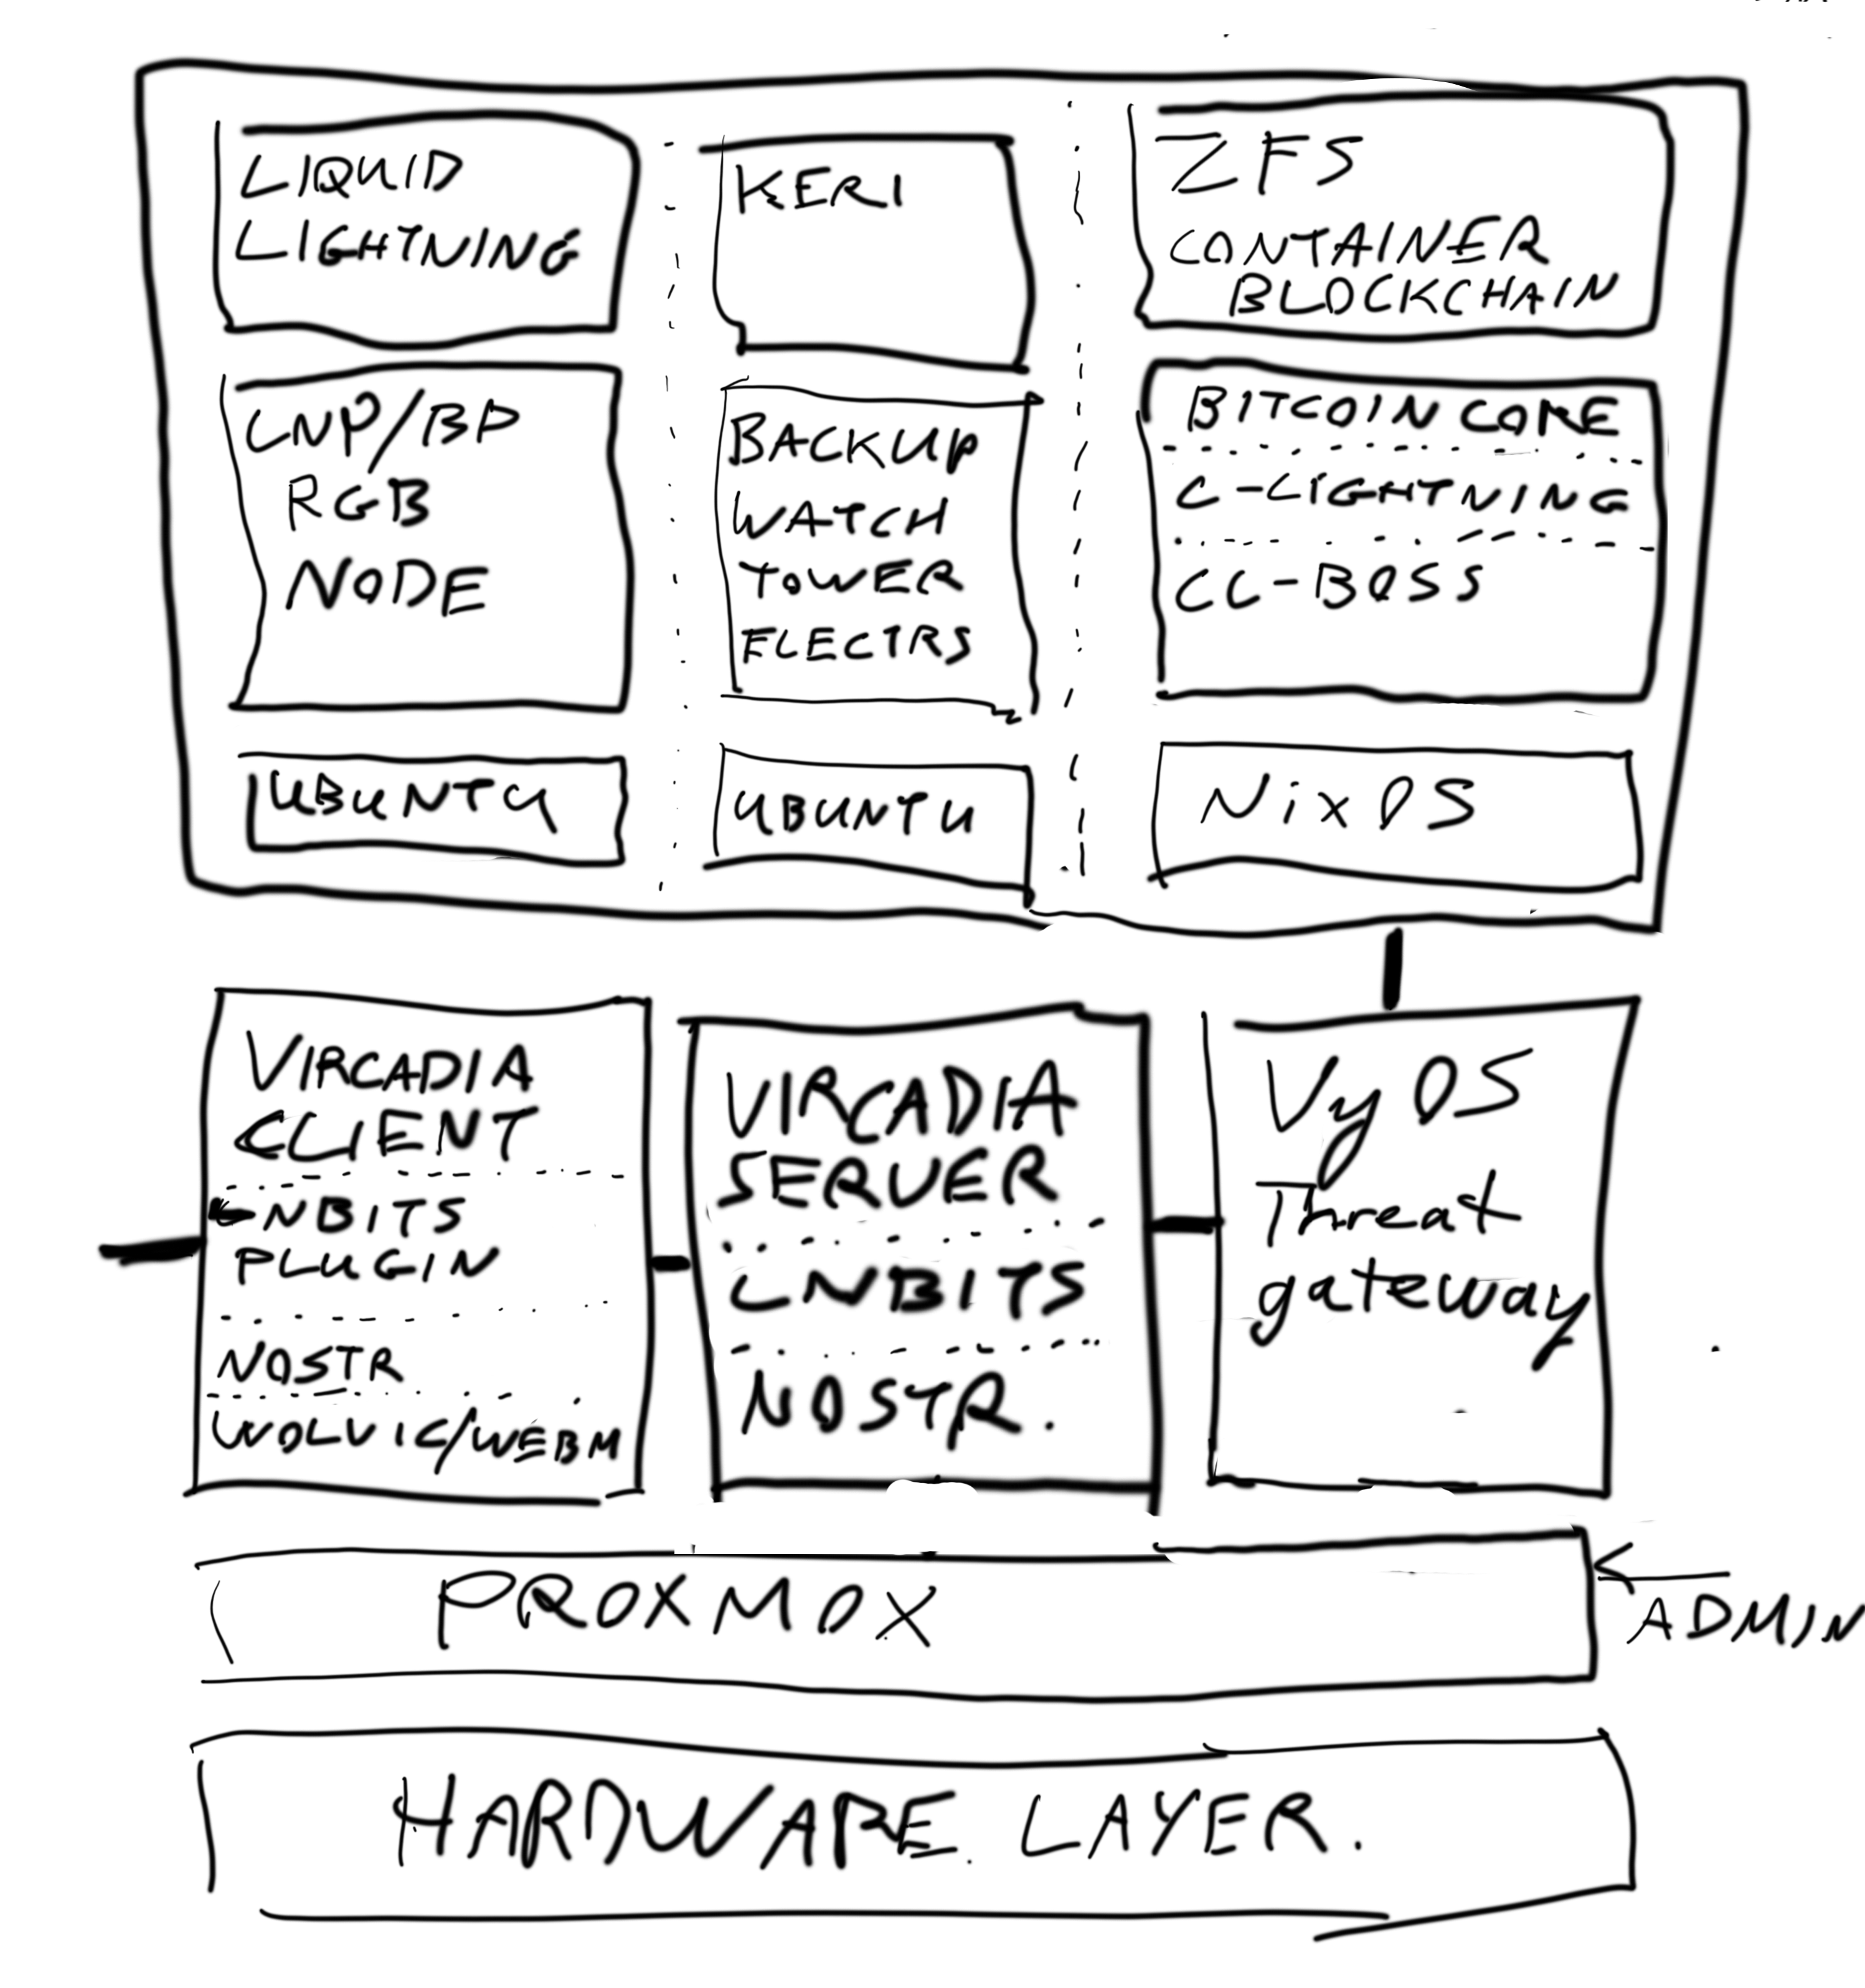
\includegraphics[width=\linewidth]{deployment}
	\caption{Proposed deployment of the software within the VMs on a single hardware system.}
	\label{fig:deployment}
\end{figure*}

\section{Networking layer}
\lipsum[50]
\subsection{Proxmox}
Proxmox open source server virtualisation allows the deployment of several virtual machines within a hardware system. Each of these VMs can have a different balance of performance, ease of use, and security. The VMs are given only the access they need to perform the task which they are specialised for. This improves overall security. Resilience is improved since elements of the cluster can be shutdown, reinstanced, and upgraded, without impacting the whole. Snapshots and backups are simplified.
\subsection{VyOS firewall}
VyOS firewall is a Proxmox aware threat management gateway and firewall which allows more nuanced interfacing with corporate systems, while maximising the security of the VM network which sits behind it i the virtual cluster.
\subsection{Privacy aspects and using TOR etc}
Currently some compromises with privacy may be necessary. Power users vs standard users. KYC/AML. 
\href{https://bitnodes.io/nodes/?q=.onion}{tor nodes}
\section{Bitcoin value management stack}
\lipsum[50]
\subsection{Bitcoin Core on NixOS}
\lipsum[50]
\subsection{Electrum server}
\href{https://blog.blockstream.com/en-esplora-and-other-alternatives-to-electrumx/}{Options on the Blockstream website}
\lipsum[50]
%\href{https://github.com/itsneski/lightning-jet}{Lightning Jet} automatic rebalance.
\subsection{C-Lightning and CLBoss}
\lipsum[50]
\subsection{LNBits with RGB and metaverse plugin}
\subsection{Backup \& Watchtower}
\lipsum[50]
\subsection{Object and media tracking: RGB}
The world database in the shared rooms in the metaverse is the global object master, with RGB client side validation inheriting and validating against these objects.\\
%Educational materials, videos, audio content and course branded objects and props are fungible tokens, authentically proved by RGB between parties. Only validated ones will be persisted in shared rooms like conferences and classes according to the room schema. Everything non compliant will be pruned. This allows educators to monetise their content, and for course participants to retain the material outside of the classroom setting where they receive them. These are fungible tokens under the RGB20 schema and can be transferred over lightning between enabled nodes. This does however imply that course participant have to run a full RGB lightning stack. This will have to be developed.\\
%NFT objects between parties like content crafted by participants (coursework, homework) are not on lightning, and will attract main chain fees. The minted material for submission will contain the nostr ID of the course participant. 
%\section{Liquid sidechain and Lightning (NFT enabled)}
%\lipsum[50]

%About Lightning Tokens: 
%https://www.youtube.com/watch?v=4k6Im5yfum0

%Detailed interview about Slashtags and %Web 3.0 aspects:
%https://twitter.com/Synonym_to/status/1481514375194292225?s=20

%Overview on all products:
%https://www.youtube.com/watch?v=5Btf_OD_3pY

%This tweetstorm is our original presentation slides:
%https://twitter.com/Synonym_to/status/1460781350441689091?s=20

%Video of the presentation:
%https://bitcointv.com/w/p1dgZcEmQQiADixvx9MoE1
\lipsum[50]
\section{Identity}
\subsection{nostr}
User authentication and sideband communication will be through nostr. This allows completely private end to end encrypted chat sessions between participants.
\section{Metaverse}
\lipsum[50]
\subsection{Vircadia}
\lipsum[50]
\subsection{Wolvic}
``The goal of the Wolvic project is to create a full-featured browser exclusively for standalone AR and VR headsets.''\\
Wolvic is a continuation of the now defunct Firefox Reality Browser project. It is open source.
\subsection{WebM}
\href{https://www.webmproject.org/about/}{Free open source web video player}	
\lipsum[50]
\section{Messengers}
Matrix, NOSTR, Juggernaut
\chapter{Example deployment }
\lipsum[50]
\section{GitHub }
\lipsum[50]

\chapter{Back to the metaverse }

It seems like the primary intersection 
Current state of the art 
Libre, Mark Carney synthetic hedgemonic currency, and Keynes baskets

\section{Potential applications }
\begin{itemize}
\item
  Art / NFT galleries with instant sales
\end{itemize}

This application allows artists and content creator communities to
display and sell NFT and fungible art to global consumer audiences,
instantly.

\begin{itemize}
\item
  Large scale conference center

  \begin{itemize}
  \item
    Academic conferences
  \item
    Political conference
  \item
    Commercial expo
  \end{itemize}
\end{itemize}

In a hypothetical virtual conference centre a true marketplace of ideas
could be enacted, with participants being paid directly by their
audience based on the proximity to the presentation.

\begin{itemize}
\item
  Group entertainment

  \begin{itemize}
  \item
    Music festivals and gigs - Pay live artists and DJs in real time
    depending on location within the extended landscape of the venue.
    Split to music producer a portion of the value
  \item
    Mixed reality theatre
  \item
    murder mystery
  \item
    Mixed reality live immersive MMORG games
  \item
    Bingo and mass participation gameshows
  \item
    Immersive brand storytelling metaverses
  \item
    Escape rooms
  \end{itemize}
\item
  Debating townhall meetings (with voting etc)
\item
  Mixed reality information metaverse

  \begin{itemize}
  \item
    AR based city tours with collectibles
  \item
    AR based collectibles for trails and heritage (museums, libraries)
    with location specific donations.
  \end{itemize}
\item
  Retail applications

  \begin{itemize}
  \item
    Proxy for physical market
  \item
    AR home delivery market interface within physical marketplaces
  \end{itemize}
\item
  Global course / Education provision
\item
  Micro tasking marketplace
\item
  Code bounty marketplace
\item
  Micro remittance role sharing (business PA / reception etc)
\item
  Careers fair with credential passing
\item
  Auctions in mixed reality
\item
  eSports and live sports
\item
  Gambling, betting markets, and financial leverage markets
\end{itemize}

\subsection{Global cybersec course delivery}
Isolating and building out one example here:
\begin{itemize}
\item Elements for the infrastructure: Economic layer, asset layer, content interface, user management, data storage, microsites loaded in Wolvin and webm, accessibility schema, network security, backups, secure messaging. Deployable framework with high modularity. Some more ossified elements for surity, some less so for malleability and open opportunity. Figure \ref{fig:globalclassroom}.
\item Course delivery in XR, how to we develop a platform, marketplace, framework for open contribution.
\item WebXR, Vircadia, any snap in metaverse middleware that is free and opensource (action to compare the two). 
\item Define an interface schema for bolting in any commercial or FOSS metaverse engine.
\item VR marketplace (outside the scope of the VR engine) without a trusted third party.
\item Cryptographically managed learning deliverables (coursework as NFT). 
\item Secure messaging and group messaging using cryptographic keys. Check this stuff with the distributed computing science people in the group (action on John)
\item work toward an exemplar MVP which is then "in the wild"
\item Platform for educators
\item Define scheme, documentation, best practice, interfaces, functional objects, pedagogy, accessibility, multi-language. 
\item Define user management system for educators and client learners.
\item Identify the pain points which current FOSS elements which need development time/money
\item separate the UI/engine from the graphical assets, and the educational / pedagogical components, accessibility, and the value and asset transfer layers.
\item Desktop systems are the primary target (low end system)
\item define schema for accessibility. Colour, subtitles, immersion concerns which can be applied to metaverse rooms through API?
\item Start to define the hybrid presentation model we favour. Avatars? Microsites? A combination of the two? Balance of guided vs unguided experience. Do we need to test the correct way to do delivery? Is there prior art we can draw on? I feel I should know. Is this part of the research that's being done here?
\item Big work package on schema vs key and user management to enforce rules in spaces. Only participants who have provably paid should have access to learning material, the ability to input into the assessment system, and the tokenised learning outcome `NFT' or proof.
\item Proof that XR system improve learning outcomes. Also that the proposed systems for micro-transactions and user and schema management give additional headroom for teaching.
\end{itemize}

Notes on buildout
The world database in the shared rooms in the metaverse is the global object master,  educational materials, videos,  audio content and branded objects are fungible tokens authentically proved by rgb client side validation between parties,  only validated ones will be persisted in shared rooms like conferences and classes according to the room schema. That allows educators to monetise their content.  That can work on lightning.  Nft objects between parties like content crafted by participants (coursework, homework) are not on lightning and will attract main chain fees but are rarer. User authentication and communication will be through nostr.

\begin{figure*}[ht]\centering % Using \begin{figure*} makes the figure take up the entire width of the page
	\includegraphics[width=\linewidth]{globalclassroom}
	\caption{Functional elements for infrastructure.}
	\label{fig:globalclassroom}
\end{figure*}

\begin{figure*}[ht]\centering % Using \begin{figure*} makes the figure take up the entire width of the page
	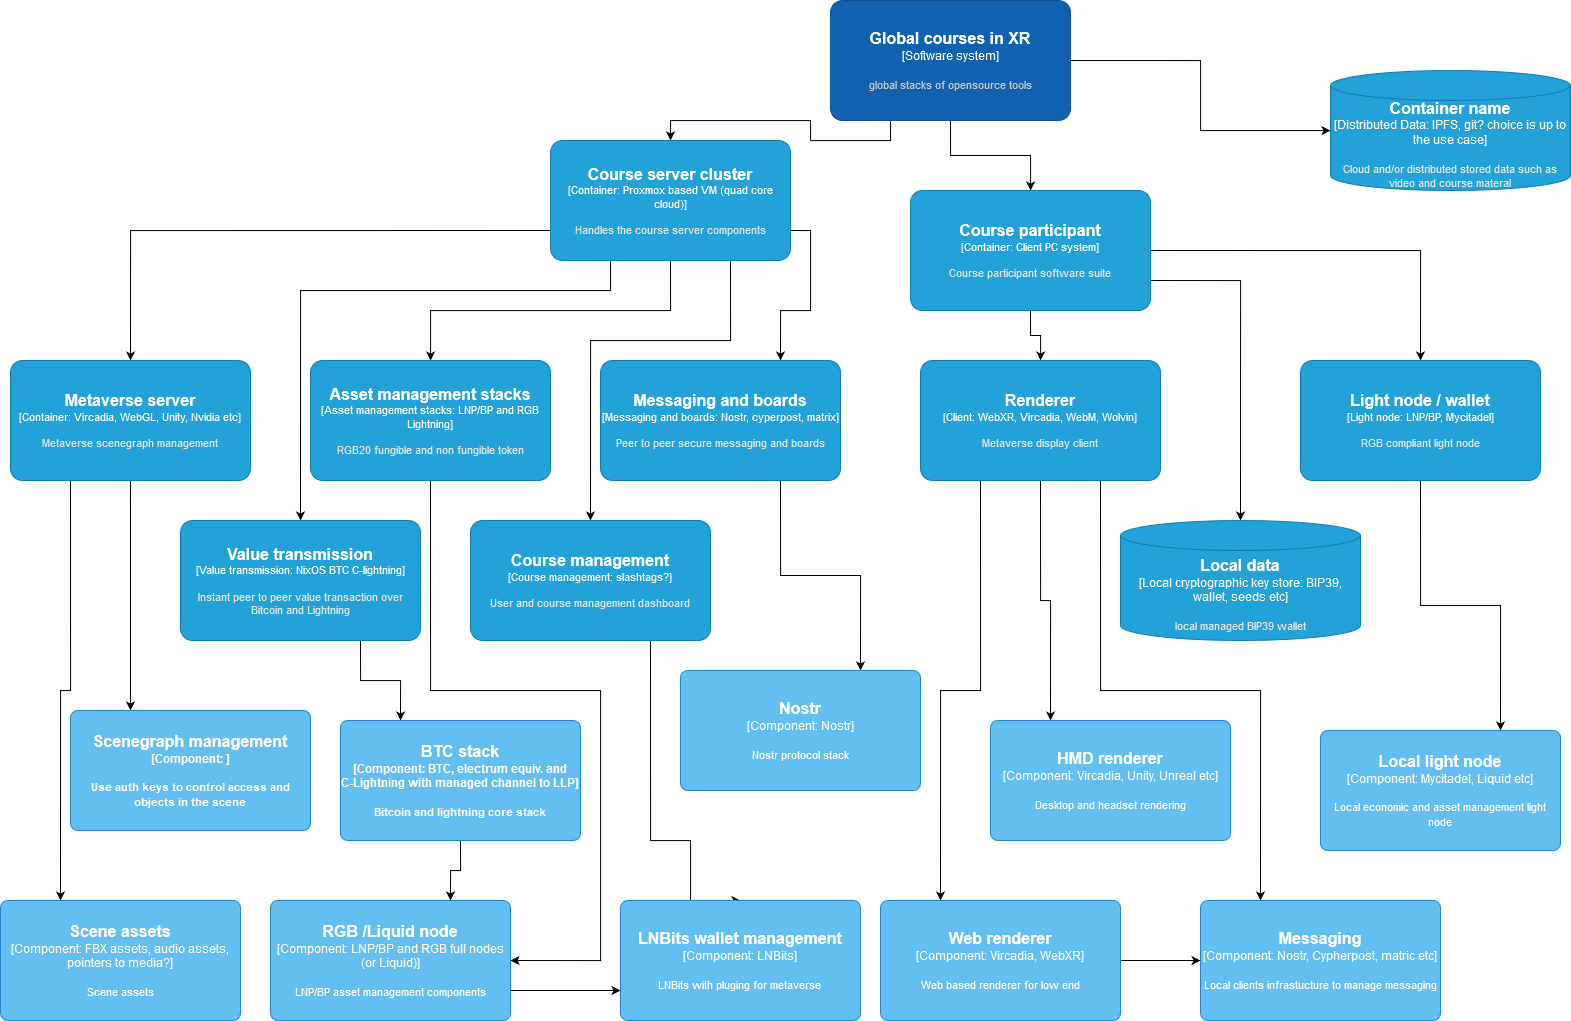
\includegraphics[width=\linewidth]{systemc4}
	\caption{Client server C4 diagrams.}
	\label{fig:globalclassroom}
\end{figure*}


\chapter{Conclusions }
%\lipsum[50]
\chapter{Future work}
%\lipsum[50]
%\lipsum[50]


\part{Guides for deploying the software}
\hypertarget{lab}{%
\section{Lab}\label{lab}}

\hypertarget{overview}{%
\subsection{Overview}\label{overview}}

This document details the process of creating the system detailed in the
accompanying paper. It is intended to be complete. It is a how to guide.

\hypertarget{summary-of-software}{%
\subsubsection{Summary of software}\label{summary-of-software}}

Summarise the software and functionality

\hypertarget{prerequisites}{%
\subsection{Prerequisites}\label{prerequisites}}

Ensure that the BIOS / firmware / etc of the hardware you intend to use
is up to date.

\hypertarget{network-details}{%
\subsection{Network details}\label{network-details}}

In the example setup provided here there are currently two networks:

\begin{enumerate}
\def\labelenumi{\arabic{enumi}.}
\tightlist
\item
  The virtual server resides in a LAN with the following details:
\end{enumerate}

192.168.x.0/24

Replace x with an integer between 0 and 254

This LAN has a gateway to the Internet and DNS server configured. Of
course, it could be replaced with a direct connection to the Internet,
though for research and development purposes it is often better to work
within a clean LAN and manage access to the Internet as required.

\begin{enumerate}
\def\labelenumi{\arabic{enumi}.}
\setcounter{enumi}{1}
\tightlist
\item
  There is a virtual network configured on the virtual machine host upon
  which virtual machines can reside:
\end{enumerate}

This virtual network is not configured to bridge with the physical
network adapter rather a virtual machine is configured as a gateway to
route IP traffic through. This provides a level of isolation. More on
this later (@todo).

\hypertarget{server-configuration}{%
\subsection{Server configuration}\label{server-configuration}}

\hypertarget{server-hardware-details}{%
\subsubsection{Server hardware details}\label{server-hardware-details}}

@todo

\hypertarget{disk-configuration-details}{%
\subsubsection{Disk configuration
details}\label{disk-configuration-details}}

@todo

\hypertarget{proxmox-ve}{%
\subsection{Proxmox VE}\label{proxmox-ve}}

\hypertarget{installation-and-configuration}{%
\subsubsection{Installation and
configuration}\label{installation-and-configuration}}

Version used: 7.1

Keep in mind that this setup uses the Proxmox VE installer
(https://www.proxmox.com/en/proxmox-ve/get-started) which, as noted on
the site, is a bare-metal installer and will erase all data on at least
one disk. There are alternative methods to install Proxmox VE but these
are not covered here.

A brief summary of the steps taken using Proxmox VE 7.1:

\hypertarget{dialogue-1}{%
\paragraph{Dialogue 1}\label{dialogue-1}}

Choose the target harddisk (/dev/sda in this case).

\hypertarget{dialogue-2}{%
\paragraph{Dialogue 2}\label{dialogue-2}}

Select country, time zone, keyboard layout.

\hypertarget{dialogue-3}{%
\paragraph{Dialogue 3}\label{dialogue-3}}

Set a password (this is the root password, see proxmox hardening
section), and email address.

\hypertarget{dialogue-4}{%
\paragraph{Dialogue 4}\label{dialogue-4}}

Select a Network Interface Card (NIC) on which the management interface
will be available and provide a hostname, IP address, gateway and DNS
server.

In this example the following settings were used:

Hostname: proxmoximus.local IP address: 192.168.x.220 / 24 Gateway:
192.168.x.254 DNS server: 192.168.x.254

Either replace x with the integer used earlier and update the last octet
of the gateway and server with that that corresponds to your setup
(assuming the setup is local and has a local dns server or forwarder) or
configure the values according to your intended setup.

Once the install has completed and the system has rebooted it is time to
begin configuring. This is done (almost entirely) via the web interface,
in this case, available at https:// proxmoximus \textbar{} 192.168.x.220
: 8006

It is also possible to login to a shell via the local terminal and SSH
(which is enabled by default @todo: in hardening, add keys and remove
ability to login with password).

\hypertarget{software-updates}{%
\subsubsection{Software updates}\label{software-updates}}

If you are in a testing and non-production environment then it is
possible access updates without a subscription as detailed here:
https://pve.proxmox.com/wiki/Package\_Repositories. Update
\texttt{/etc/apt/sources.list} as detailed under the Proxmox VE
No-Subscription Repository. This can be achieved via the local terminal,
SSH or web interface (via Shell option).

For example, edit the file:

\texttt{nano\ /etc/apt/sources.list}

Add the following:

\begin{verbatim}
# PVE pve-no-subscription repository provided by proxmox.com,
# NOT recommended for production use
deb http://download.proxmox.com/debian/pve bullseye pve-no-subscription
\end{verbatim}

To the existing:

\begin{verbatim}
deb http://ftp.uk.debian.org/debian bullseye main contrib

deb http://ftp.uk.debian.org/debian bullseye-updates main contrib

# security updates
deb http://security.debian.org bullseye-security main contrib
\end{verbatim}

Resulting in:

\begin{verbatim}
deb http://ftp.debian.org/debian bullseye main contrib
deb http://ftp.debian.org/debian bullseye-updates main contrib

# PVE pve-no-subscription repository provided by proxmox.com,
# NOT recommended for production use
deb http://download.proxmox.com/debian/pve bullseye pve-no-subscription

# security updates
deb http://security.debian.org/debian-security bullseye-security main contrib
\end{verbatim}

The Proxmox VE system will now retrieve updates for both itself and the
base Debian system.

Then from a shell run:

\begin{verbatim}
$ apt update
$ apt upgrade
\end{verbatim}

@todo: determine if system needs a reboot

\hypertarget{proxmox-ve-hardening}{%
\subsubsection{Proxmox VE hardening}\label{proxmox-ve-hardening}}

Links

@todo

Adding users

Add SSH keys and remove ability to login with password

\hypertarget{setup-an-internal-only-network-in-proxmox-ve}{%
\subsection{Setup an internal only network in Proxmox
VE}\label{setup-an-internal-only-network-in-proxmox-ve}}

From the Web GUI navigate to Datacenter - \textgreater{} your server
-\textgreater{} Network

From the menu select Create then Linux Bridge

Input the desired IPv4/CIDR in this case 192.168.y.0/24 and add a
comment if desired (``Internal network'' was used here). Note that y
must not be the same as x previously used.

Name was left as vmbr1

Credit:
https://dannyda.com/2020/06/01/how-to-create-an-internal-only-isolated-network-for-guest-os-virtual-machines-vm-on-proxmox-ve-pve-like-in-vmware-workstation-host-only-network-but-different/

\hypertarget{install-and-configure-internet-gateway-server-virtual-machine}{%
\subsection{Install and configure Internet gateway server virtual
machine}\label{install-and-configure-internet-gateway-server-virtual-machine}}

VyOS was selected (https://vyos.io/)

\hypertarget{create-an-iso-of-the-stable-version-as-of-writing-1.3.0}{%
\subsubsection{Create an ISO of the stable version (as of writing
1.3.0)}\label{create-an-iso-of-the-stable-version-as-of-writing-1.3.0}}

@todo: the built version seemed to be a nightly release, is it possible
to add a tag to get a stable build?

Follow the build instructions:

https://docs.vyos.io/en/latest/contributing/build-vyos.html

This document does not list this version (goes up to 10 ``buster'') but
Debian 11 ``bullseye'' was successfully used in this setup.

Run the following commands:

\begin{verbatim}
$ apt install git
$ apt install build-essential
\end{verbatim}

Follow the instructions here
https://docs.docker.com/engine/install/debian/ to install Docker

Run the following commands:

\begin{verbatim}
$ git clone -b equuleus --single-branch https://github.com/vyos/vyos-build

$ docker run --rm -it --privileged -v $(pwd):/vyos -w /vyos vyos/vyos-build:equuleus bash
\end{verbatim}

Then in the Docker terminal run the following commands:

\begin{verbatim}
./configure --architecture amd64

sudo make iso
\end{verbatim}

\hypertarget{upload-the-iso-image-to-the-proxmox-ve-server}{%
\subsubsection{Upload the ISO image to the Proxmox VE
server}\label{upload-the-iso-image-to-the-proxmox-ve-server}}

\begin{enumerate}
\def\labelenumi{\arabic{enumi}.}
\item
  Via the web GUI navigate to Datacenter -\textgreater{} your server
  -\textgreater{} local.
\item
  In the right hand pane select ISO Images and then upload.
\item
  Upload the ISO image
\end{enumerate}

Tip: you can also pass the checksum to the Proxmox VE upload tool

\hypertarget{create-vyos-virtual-machine}{%
\subsubsection{Create VyOS virtual
machine}\label{create-vyos-virtual-machine}}

\begin{enumerate}
\def\labelenumi{\arabic{enumi}.}
\item
  From the top right of the web GUI select Create VM
\item
  In the appearing dialogue type a Name ``VyOS'' and optionally select
  advanced and Start at boot
\item
  On the next tab select the target ISO image
\item
  On the System tab leave everything as default
\item
  n the Disk tab leave the defaults (this exceeds requirements
  https://docs.vyos.io/en/latest/installation/install.html)
\item
  On the CPU tab:

  Sockets: 1, Cores: 2
\item
  On the Memory tab

  Memory: 4096MiB
\item
  On the Network tab

  Choose the bridge with the internet vmbr0 (it is possible to add the
  second later) and leave the defaults including firewall

  Confirm all the settings on the next tab but \textbf{do not} select
  start after created

  Navigate to the newly created VM on the left-hand pane then selected
  Hardware from the menu that is presented on the right. Choose Add and
  then Network Device. In the dialogue that appears select the Internal
  network bridge (vmbr1 in this case) that was created earlier and leave
  all other options as is.

  So, the VM will have the following Network Devices:

  net0: Internet

  net1: Internal only
\item
  Start the VM and connect the console (top right)
\item
  Login with vyos and vyos

  Run the command:

\begin{verbatim}
$ install image
\end{verbatim}
\item
  Follow the instructions
\item
  Set the CD/DVD to none in Web GUI
\item
  Reboot
\end{enumerate}

\hypertarget{configure-vyos}{%
\subsubsection{Configure VyOS}\label{configure-vyos}}

Open a noVNC window to the host

Login with vyos and vyos

Switch to configure mode:

\begin{verbatim}
vyos@vyos$ configure
vyos@vyos#
\end{verbatim}

Then configure as desired. Below is configuration used in the setup here
(if you use for inspiration do take care to replace the x and y octet
values correctly with previously chosen values. The z octet value should
be something unused in the outside LAN for which the host is physically
connected):

\begin{verbatim}
set interfaces ethernet eth0 address '192.168.x.z/24'
set interfaces ethernet eth0 description 'OUTSIDE'
set protocols static route 0.0.0.0/0 next-hop 192.168.x.254 distance 1
set service dns forwarding system
set service dns forwarding name-server 192.168.x.254
set service dns forwarding listen-address 192.168.y.1
set service dns forwarding allow-from 192.168.y.0/24
set system name -server 192.168.x.254

set interfaces ethernet eth1 address '192.168.y.1/24'
set interfaces ethernet eth1 description 'INSIDE'

set nat source rule 100 outbound-interface eth0
set nat source rule 100 source address 192.168.y.0/24
set nat source rule 100 translation address masquerade

set service ssh listen-address 0.0.0.0
\end{verbatim}

Once done remember to commit the config (correcting any
misconfiguration) and save.

\begin{verbatim}
commit
save
\end{verbatim}

Inspiration for the above was taken from:
https://bertvv.github.io/cheat-sheets/VyOS.html

@todo: hardening, IDS, IPS

\hypertarget{install-and-configure-a-debian-virtual-machine}{%
\subsection{Install and configure a Debian virtual
machine}\label{install-and-configure-a-debian-virtual-machine}}

This VM can be used for various tasks such as software compilation and
testing of the networks. In this setup the Debian VM was used to test
connectivity to the VyOS gateway and the Internet. It is also used in
the subsequent stages to deploy a nix-bitcoin node.

In Proxmox VE create a new virtual machine and configure the network
device to use the bridge `vmbr1'.

Then install Debian and configure the network adapter within the VM with
the following settings:

IP address: 192.168.y.2 Gateway: 192.168.y.1 DNS: 192.168.y.1

Test that the VM has Internet connectivity.

\hypertarget{deploying-the-nix-bitcoin-node}{%
\subsection{Deploying the nix-bitcoin
node}\label{deploying-the-nix-bitcoin-node}}

This deployment follows the documentation:

https://github.com/fort-nix/nix-bitcoin/\#get-started

Take note of the hardware requirements:

https://github.com/fort-nix/nix-bitcoin/blob/master/docs/hardware.md

In the main, the install guide
(https://github.com/fort-nix/nix-bitcoin/blob/master/docs/install.md) is
followed verbatim and notes with a reference to particular sections are
added where appropriate.

Optional - a small exception in regards to this setup is that a separate
virtual disk (located on a different physical drive mirror (RAID 1)) was
used to store the bitcoin database - this is optional and details are
provided on how to achieve it. Also detailed is how to configure the
network when using the minimal image.

\hypertarget{acquiring-nixos}{%
\subsubsection{Acquiring NixOS}\label{acquiring-nixos}}

Following
\href{https://github.com/fort-nix/nix-bitcoin/blob/master/docs/install.md\#1-nixos-installation}{section
1.1} make sure the latest NixOS is obtained i.e.~do not just copy the
whole wget command outright and make sure to verify the hash against
trusted sources before using the image.

Download the minimal ISO image (https://nixos.org/download.html)

Verify the hash

Upload the ISO to
\protect\hyperlink{ux5cux23ux5cux23Upload-the-ISO-image-to-the-Proxmox-VE-server}{Proxmox
VE server}

\hypertarget{create-a-new-vm}{%
\subsubsection{Create a new VM}\label{create-a-new-vm}}

Name: NixOS

Follow the setup and leave everything as default until the CPU page. The
following configuration was used, which should exceed the minimum
requirements:

Cores: 4

Memory: 4096MiB = 4.2GB

Network: vmbr1 (Internal Network)

Do NOT check the select the start the VM checkbox

Next, an additional drive will be configured in Proxmox VE. This will
then be used to store the bitcoin database within the NixOS VM.

Select Datacenter -\textgreater{} server name and then from the right
pane Disks -\textgreater{} LVM-Thin. Then select Create: Thinpool

From the dialogue select the disk and type a name ``data'' was used in
this setup. This provisions a vg with the name \emph{data} and a name
\emph{data} @todo: review

Navigate back to the VM created and choose Hardware and then Add
-\textgreater{} Hard Disk

Choose ``data'' from Storage and then set the size to 560 GiB which
equates to about 600GB

Now, continue from section 1.3 in the install instructions

Start the VM and connect a console

\texttt{sudo\ -i}

With the SeaBios that was used in this setup the file does not exist and
Legacy Boot (MBR) should be followed (option 2)

Note: no consideration is currently given for encrypted partitions
within the Proxmox VE setup

Enable the OpenSSH daemon

\begin{verbatim}
services.openssh.permitRootLogin = "yes";
\end{verbatim}

Configure the network config in configuration.nix (remember to replace y
with the chosen value)

\begin{verbatim}
  networking.useDHCP = false;
  networking.interfaces.ens18.useDHCP = false;

  networking.interfaces.ens18.ipv4.addresses = [ {
    address= "192.168.y.3";
    prefixLength = 24;
  } ];
  networking.defaultGateway = "192.168.y.1";
  networking.nameservers = ["192.168.y.1"];
  networking.hostName = "nixicon";
\end{verbatim}

Although the IP above will be assigned once the nix-bitcoin is deployed
the installation cannot continue without a connection to the Internet so
that needs to be configured:

\begin{verbatim}
$ ifconfig ens18 192.168.y.3
$ ifconfig ens18 255.255.255.0
$ ip route add 192.168.y.0/24 dev ens18 scope link src 192.168.y.3
\end{verbatim}

Then add the nameserver:

\begin{verbatim}
nano /etc/resolv.conf
\end{verbatim}

Add:

\begin{verbatim}
nameserver 192.168.y.1
\end{verbatim}

Once the above is complete and successful networking is verified

Run the following command:

\texttt{nixos-install}

Set the root password and then reboot.

\hypertarget{configure-the-additional-drive-optional}{%
\subsubsection{Configure the additional drive
(optional)}\label{configure-the-additional-drive-optional}}

As the additional drive was not configured at the time of the install
then the parted utility will need to be available. To achieve this, edit
the configuration.nix file

\texttt{nano\ /etc/nixos/configuration.nix}

and add the following:

\begin{verbatim}
environment.systemPackages = with pkgs; [
    parted
];
\end{verbatim}

Then issue the following command:

\texttt{nixos-rebuild\ switch}

Determine the desired drive, fdisk can assist:

\texttt{fdisk\ -l}

Note: in this sytem the desired drive is /dev/sdb with 560GiB capacity
but sdx is used in the following examples:

Then partition:

\texttt{parted\ /dev/sdx}

\begin{verbatim}
(parted) mklabel msdos
(parted) mkpart primary
File system type? ext4
Start? 0%
End? 100%
quit
\end{verbatim}

(note: it is possible to combine the above as a single line command)

Then create the file system:

\texttt{mkfs.ext4\ -L\ data\ /dev/sdx1}

Make a note of the UUID as this will be used in the next steps to mount
the volume

\hypertarget{create-port-forwarding-rules-for-ssh-optional}{%
\subsubsection{Create port forwarding rules for SSH
(optional)}\label{create-port-forwarding-rules-for-ssh-optional}}

Providing SSH access to the VMs from outside the private network makes
it easier to configure them (ability to copy and paste UUIDs etc.)

This involve updates to VyOS configuration and can be temporary.

Login to the vyos, you should be able do this from your local machine
now as apposed to the console

ssh vyos@192.168.x.z

\hypertarget{debian}{%
\paragraph{Debian}\label{debian}}

192.168. y .2

The following commands were issued to the VyOS router (obiously
replacing y with the value chosen earlier)

\begin{verbatim}
configure

set nat destination rule 12 description 'Port Forward: 2222 to 22 SSH on 192.168.y.2'
set nat destination rule 12 destination port '2222'
set nat destination rule 12 inbound-interface 'eth0'
set nat destination rule 12 protocol 'tcp'
set nat destination rule 12 translation address '192.168.y.2'
set nat destination rule 12 translation port '22'

commit
\end{verbatim}

Now test

Note: for the Debian VM the user account may need to be added to the SSH
user group

Note: you could SSH from Debian to all other hosts

\hypertarget{nixos}{%
\paragraph{NixOS}\label{nixos}}

192.168. y .3

Assuming access to the Debian VM via SSH is working then from the same
VyOs configure session issue the following:

\begin{verbatim}
set nat destination rule 13 description 'Port Forward: 2223 to 22 SSH on 192.168.y.3'
set nat destination rule 13 destination port '2223'
set nat destination rule 13 inbound-interface 'eth0'
set nat destination rule 13 protocol 'tcp'
set nat destination rule 13 translation address '192.168.y.3'
set nat destination rule 13 translation port '22'

commit
\end{verbatim}

Test and if all is well, save the VyOS configuration:

\begin{verbatim}
save
\end{verbatim}

Credit: https://support.vyos.io/en/kb/articles/nat-principles

Having SSH access to both the Debian and NixOS VMs will make the next
stages of the process a little easier

@todo hardening (SSH e.g.~add keys, remove plain text or remove SSH
access entirely)


\stopcontents[part] % Manually stop the 'part' table of contents here so the previous Part page table of contents doesn't list the following chapters

\part{Appendix}
\section{Acknowledgements and thanks}

\section{Author Biographies}
\noindent\fcolorbox{red}{lightgray}{%
\begin{minipage}{\dimexpr0.66\textwidth-2\fboxrule-2\fboxsep\relax}
Dr John O`Hare is a results driven, certified Prince2 Agile Practitioner. Leveraging proven analytical ability, and drawing on 23 years of experience at the University of Salford.  Successful as a leader and an influential team member in both project and customer-facing roles. As a product manager he specialises in systems design, procurement, tendering and bid writing for research funding, running complex heterogeneous research systems, research and development, and supporting academic staff / research students to undertake theirs. Completed a PhD in \href{https://www.researchgate.net/profile/John-Ohare/publication/332029624_Telethrone_a_situated_display_using_retro-reflection_based_multi-view_toward_remote_collaboration_in_small_dynamic_groups/links/5c9ba02645851506d72ff380/Telethrone-a-situated-display-using-retro-reflection-based-multi-view-toward-remote-collaboration-in-small-dynamic-groups.pdf}{``Attention in Telepresence''}, uniting the gaze of remote collaborators, through furniture. Recently pursuing research opportunities in value transfer mechanisms for `Metaverses'.
\end{minipage}}%
\begin{minipage}{0.67\textwidth}
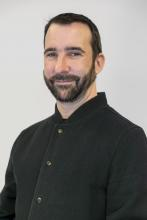
\includegraphics[width=23ex]{JOH}
\end{minipage}

%----------------------------------------------------------------------------------------
%	BIBLIOGRAPHY
%----------------------------------------------------------------------------------------

\chapterimage{} % Chapter heading image
\chapterspaceabove{2.5cm} % Whitespace from the top of the page to the chapter title on chapter pages
\chapterspacebelow{2cm} % Amount of vertical whitespace from the top margin to the start of the text on chapter pages

%------------------------------------------------

\chapter*{Bibliography}
\addcontentsline{toc}{chapter}{\textcolor{ocre}{Bibliography}} % Add a Bibliography heading to the table of contents

\section*{Articles}
\addcontentsline{toc}{section}{Articles} % Add the Articles subheading to the table of contents

\printbibliography[heading=bibempty, type=article] % Output article bibliography entries

\section*{Books}
\addcontentsline{toc}{section}{Books} % Add the Books subheading to the table of contents

\printbibliography[heading=bibempty, type=book] % Output book bibliography entries

%----------------------------------------------------------------------------------------
%	INDEX
%----------------------------------------------------------------------------------------

\cleardoublepage % Make sure the index starts on an odd (right side) page
\phantomsection
\addcontentsline{toc}{chapter}{\textcolor{ocre}{Index}} % Add an Index heading to the table of contents
\printindex % Output the index

\end{document}
